\documentclass[11pt,twoside,onecolumn,titlepage,openbib]{book}
\usepackage[a4paper, top=2cm, bottom=2cm, left=2.5cm,right=2cm]{geometry}
\usepackage[latin1]{inputenc}
\usepackage[dutch]{babel} % Gebruik Nederlandse spelling
\usepackage{graphicx} % Om figuren (.eps, .png, .pdf) in te laden
\usepackage{makeidx}
%\usepackage[pdftex]{graphicx}
\newcommand{\HRule}{\rule{\linewidth}{0.5mm}}
\usepackage{fancyhdr}
\usepackage{amsmath} % Gebruikg geavanceerde wiskundige symbolen- en macro-bibliotheek
\usepackage{amsfonts} % Gebruikg geavanceerde wiskundige symbolen- en macro-bibliotheek
\usepackage{amssymb} % Gebruikg geavanceerde wiskundige symbolen- en macro-bibliotheek

\pagestyle{fancy}
\fancyhead{}
\fancyfoot{}
\fancyhead[LE,RO]{\thepage}
\fancyhead[RE]{\bfseries\leftmark}
\fancyhead[LO]{\bfseries{Thinkpad T410, 20110}}
\fancyfoot[C]{\bfseries{CLW Don Bosco - Valkenveld 70  - 2610 Wilrijk}}
\renewcommand{\headrulewidth}{0.4pt}
\renewcommand{\footrulewidth}{0.4pt}
% \title{Drupal 6.15 on Fedora 12}
% \author{Mitchell Huyssen\\
%   Afdeling Netwerkassistent,\\
%   CLW Don Bosco,\\
%   Wilrijk\\
%   \texttt{mitchell.huyssen@donboscowilrijk.be}}
% \date{\today}

%\setlength{\headheight}{15pt} % my addition to fix headhight is to small
% warning

\makeindex

\begin{document}

\frontmatter

\begin{titlepage}
\begin{center}
\textsc{\Large }\\[1.5cm]
\textsc{\Large Eindwerk Netwerkassistent 2011}\\[0.5cm]
% Title
\HRule \\[0.8cm]
{ \huge \bfseries Thinkpad T410}\\[0.4cm]
\HRule \\[1.5cm]
 \begin{figure}[!t]
    \centering
   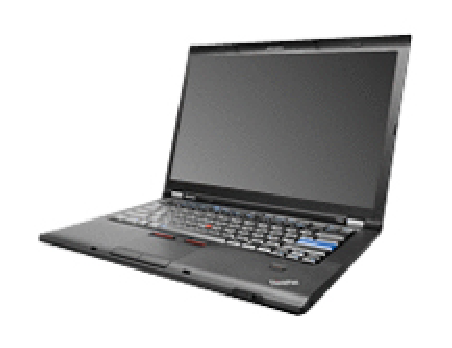
\includegraphics[scale=0.7]{01-lenovo-laptop}
 %  \small \\Drupal
 \end{figure}
\textsc{\Large }\\[2.5cm]
% Author and supervisor
\begin{minipage}{0.4\textwidth}
\begin{center}
\large Robert \textsc{Keersse}\\
\texttt{robert.keersse@donboscowilrijk.be}\\
\texttt{ }\\
Opleiding Netwerkassistent\\
Don Bosco Werken en Leren\\
2610 - Wilrijk - Antwerpen
\end{center}
\end{minipage}
\vfill
% Bottom of the page
\end{center}
\end{titlepage}

\tableofcontents
\listoffigures
\newpage
\chapter*{Voorwoord}
Allereerst wil ik mijn dank uitspreken over mijn begeleiders, \ldots, \ldots
en \ldots bij \ldots. Niet alleen heb ik van hen ongeloofelijk veel
technische kennis opgedaan, maar ook leren werken, en zeker, werk leren zien.
\\\\
Graag wil ik mijn leerkrachten bedanken voor hun volharding en steun. De heer
Peeters, waar ik van heb ``leren lezen en schrijven'' en in bijzonder dat ik mocht
proeven van zijn kennis over PHP en SQL. Wat me het meest bijblijft van de
theorie lessen gegeven door de heer Jennes, is dat deze meestal ver boven mijn
petje gingen, nochthans begrijp ik nu wel dat je de lat nooit hoog genoeg kan
leggen.
\\\\
Mijn eindwerk over \ldots is blablabla \ldots. De
praktische installatie kan je terugvinden in de bijlage.
\\\\
blablabla. Het is niet mijn bedoeling dat dit eindwerkje een
volledige beschrijving geeft wat je allemaal met \ldots kan, het kan misschien
dienen als startpunt voor \ldots.

\begin{flushright}
Robert Keersse\\juni 2011
\end{flushright}


\mainmatter
\part{Inleiding}
\chapter{CMS}
Het contentmanagementsysteem \index{contentmanagementsysteem}(CMS) waarover mijn eindwerk gaat is
Drupal, dit maakt gebruikt van de scripttaal 'PHP' met een bijbehorende SQL database, ik maak hierbij gebruik van
MySQL. Het is eveneens mogelijk gebruik te maken van andere databases. Het door
mij gekozen besturingssysteem is Linux Fedora 12.
\section{Contentmanagementsysteem}
Een content-beheersysteem of contentmanagementsysteem is een softwaretoepassing,
meestal een web-applicatie, die het mogelijk maakt dat mensen eenvoudig, zonder 
veel technische kennis, documenten en gegevens op internet kunnen publiceren. 
Als afkorting wordt ook wel CMS gebruikt, naar het Engelse content management system. 
Een functionaliteit van een CMS is dat gegevens zonder lay-out (als platte tekst) 
kunnen worden ingevoerd, terwijl de gegevens worden gepresenteerd aan bezoekers met 
een lay-out door toepassing van sjablonen. Een CMS is vooral van belang voor websites 
waarvan de inhoud regelmatig aanpassing behoeft, en de inhoud in een vaste lay-out 
wordt gepresenteerd aan bezoekers. De meeste grote bedrijven gebruiken voor hun website 
tegenwoordig een CMS.
\subsection{Onderdelen}
Een CMS bestaat ten minste uit de volgende onderdelen:
\begin{itemize}
  \item een (bijna altijd afgeschermde) administratiemodule, waar gegevens kunnen worden ingevoerd, verwijderd of aangepast.
  \item een database of een andere vorm van opslag van de gegevens.
  \item een presentatiemodule, waar de ingevoerde gegevens door bezoekers
  kunnen worden bekeken.
\end{itemize}
Daarnaast kunnen er andere onderdelen zijn:
\begin{itemize}
  \item een zoekmodule
  \item een inlogmodule voor bezoekers, als het niet gewenst is dat anonieme bezoekers toegang hebben tot de inhoud
  \item een beheersmodule voor de gegevens van geautoriseerde bezoekers (en beheerders)
  \item een beheersmodule voor de presentatiesjablonen
  \item een module om persoonlijke informatie aan de bezoeker te tonen (personalisaties)
  \item een module om centraal artikelen aan te kunnen maken die op verschillende pagina's getoond kunnen worden
  \item \ldots
\end{itemize}

\section{Waarom Drupal}
\begin{itemize}
  \item Vele functies en uitbreidingsmogelijkheden.
  \item Effici\"ent en effectief: met relatief weinig moeite kan u veel
  bereiken. Drupal gebruiken bespaart tijd. Er hoeft niet steeds vanaf nul te worden ontwikkeld.
  \item Het uiterlijk is flexibel aan te passen. Hiervoor zijn vele 'Themes'
  beschikbaar. 'Themes' zijn eenvoudig en eindeloos aan te passen aan specifieke wensen.
  \item Grote actieve community, plus een groot netwerk van service-aanbieders
  geven vertrouwen in de continu\"\i teit van Drupal.
\end{itemize}

\subsection{Voor managers}
Door de vele functies en uitbreidingsmogelijkheden is Drupal bruikbaar voor
uiteenlopende doeleinden. Van marketing-inspanningen tot intern communicatiegebruik. 
Voor informerende websites, maar ook voor communicatie tussen verschillende groepen. 
Drupal is makkelijk uitbreidbaar. Als bepaalde functionaliteit nog niet beschikbaar is, 
dan zijn er veel mogelijkheden om ontwikkelaars in te huren om een of meerdere extra 
modules te bouwen. Er is een grote en gedreven community met diverse ervaren leden 
die u graag van dienst zijn. De actieve community en een groot netwerk van 
service-aanbieders geven de vele gebruikers bovendien vertrouwen in de
continu\"\i teit van Drupal. Drupal is ook vlot te beheren. Het
toegangscontrolesysteem kan eenvoudig worden aangepast aan uw organisatiestructuur. 
Zodat iedereen precies de nodige toegang heeft.

\subsection{Voor beheerders}
Het staat bekend als effici\"ent en effectief: met relatief weinig moeite kan
u veel bereiken. Drupal biedt gebruikers een eenvoudig te bedienen
gebruikersinterface, die ook flexibel en uitbreidbaar. Zo kan u
verschillende typen inhoud beheren: tekst, afbeeldingen, video, kalenders, enqu\^etes, forums,
\ldots De uitbreidingsmogelijkheden maken het eenvoudig om snel nieuwe inhoudstypen toe
te voegen en daarmee de functionaliteit te verbeteren.

\subsection{Voor ontwikkelaars}
Website-ontwikkelaars waarderen Drupal omdat het hen toelaat effici\"ent te
werken. Drupal gebruiken bespaart tijd. Er hoeft niet steeds vanaf nul te worden ontwikkeld. 
Omdat zoveel mensen aan Drupal bijdragen, bevat het goede API's. De grote verzameling van 
modules wordt voortdurend uitgebreid en bijgewerkt. De Drupal-community is een grote groep 
van vrijwilligers die met plezier informatie uitwisselen om een klus te klaren.

\subsection{Voor grafische vormgevers}
Het uiterlijk van een Drupal-website is flexibel aan te passen. Hiervoor zijn
vele 'themes' beschikbaar. 'Themes' zijn eenvoudig en eindeloos aan te passen aan specifieke wensen.


\section{PHP}
PHP \index{server-side scriptingtaal - PHP}is een server-side scriptingtaal, die
hoofdzakelijk wordt gebruikt om op de webserver dynamische webpagina's te cre\"eren, is voor de gebruiker
onzichtbaar. Alleen het resultaat is zichtbaar en dat ziet eruit als een gewone HTML-pagina. 
De voordelen van PHP zijn: het is open source, het is zeer populair en makkelijk 
te leren en er is een brede ondersteuning mogelijk op het internet.
\subsection{Geschiedenis}
PHP werd in 1994 ontwikkeld door Rasmus Lerdorf. De eerste publieke versie werd uitgegeven in 1995, 
alsook versie 2. Zeev Suraski en Andi Gutmans, twee Isra\"elische ontwikkelaars
aan de Technion IIT, herschreven de parser in 1997 en vormden de basis voor PHP 3 en veranderde hiermee de naam in PHP: 
Hypertext Preprocessor. Het ontwikkelteam bracht PHP/FI 2 officieel in November 1997 uit, na maanden van beta-tests. 
Hierna begon de publieke test van PHP 3 en in juni 1998 werd PHP 3 officieel uitgebracht. Suraski en Gutmans begonnen 
hierna met het herschrijven van de PHP parser, met de Zend Engine in 1999 als resultaat. Hiermee werd Zend Technologies 
opgericht in Ramat Gan, Isra\"el.
Op 22 mei 2000 werd PHP 4, aangedreven door Zend Engine 1.0, uitgebracht. Op 13 juli 2004 werd PHP 5 uitgebracht, 
aangedreven door de nieuwe Zend Engine II.
Ondanks dat PHP 5 al sinds 2004 beschikbaar is, gebruiken veel webservers pas sinds begin 2007 PHP5, omdat eerdere versies 
niet stabiel genoeg waren. De meest recente stabiele versie is 5.3.1 (19 november 2009). In deze versie zijn er ook veel 
bug-fixes gedaan. De belangrijkste kenmerken van PHP 5 zijn het verbeterde objectgeori\"enteerd programmeren, de hogere 
snelheid, de mogelijkheid om SQLite aan te spreken en de vernieuwde XML-bibliotheek.
\subsection{Gebruik}
PHP wordt veel gebruikt om op webservers dynamische webpagina's te
cre\"eren. Andere bekende server-side scripttalen zijn Java Server Pages (JSP), Coldfusion en Active Server Pages (ASP). De code van de pagina wordt op de server uitgevoerd, 
en het resultaat wordt naar de computer van de bezoeker gestuurd en in de webbrowser getoond. Dit in tegenstelling tot 
client-side scripting (zoals Javascript), waarbij de webbrowser eerst de pagina van de webserver downloadt en vervolgens 
zelf (op de computer van de bezoeker) code uitvoert.
\\
Bij het oproepen van een PHP-document op de server wordt (op de server) eerst de in het document opgenomen PHP-code uitgevoerd. 
Dit gebeurt door de PHP-parser (de PHP-engine). Het resultaat (meestal HTML) wordt door de webserver naar de browser gestuurd. 
PHP kan echter ook andere documenttypen versturen. PHP-documenten hebben meestal de extensie .php, maar ook de oudere extensies 
worden nog (weliswaar sporadisch) gebruikt.
\\
PHP ondersteunt ook diverse extensies die (in de Windows-versie) als een simpele DLL kunnen worden geactiveerd, om daarna het 
php.ini aan te passen. Alle documentatie is in de PHP-handleiding te vinden. Onder andere door de gemakkelijk bereikbare 
documentatie (centraal op een locatie) is PHP populair geworden onder webprogrammeurs.
\\
PHP wordt zeer veel gebruikt in combinatie met Linux, Apache en MySQL, afgekort tot LAMP. De LAMP-architectuur is zeer succesvol 
op het internet. Het komt ook wel eens voor dat men Windows gebruikt in plaats van Linux. WAMP is hierbij de afkorting voor 
systemen die Windows gebruiken en er wordt wel eens de afkorting MAMP gebruikt voor de Macintosh. Ook zijn er kant en klare 
programma's die een volledige WAMP omgeving installeren. Voorbeelden hiervan zijn WAMP en XAMPP.

\subsection{Voorbeeld}
\begin{verbatim}
<?php
   $drupaltekst = "Dit is GEEN Drupal website";
   echo $drupaltekst;
  // hier zal dan uiteindelijk "Dit is GEEN Drupal website" op de site komen te staan
?>
\end{verbatim}

\subsection{OOP \index{Object Oriented programming}}
PHP wordt vanwege het lage instapniveau gezien als een van de makkelijkste webtalen en voorziet tegelijk in grote 
doorgroeimogelijkheden. Zo is het met PHP ook mogelijk objectgeori\"enteerd (OO,Object Oriented) te programmeren. 
Bij OO-programmeren (OOP) maakt men klassen van waaruit weer objecten gemaakt kunnen worden. De klassen zijn als het ware 
een recept, een beschrijving van het object. Een bouwplattegrond van een fiets is vergelijkbaar met een klasse en de fiets 
zelf is vergelijkbaar met een object. In de klasse zijn de onderdelen van de fiets beschreven (properties, bijv. wielen, 
trappers, etc.) en de mogelijkheden van een fiets (methods, bijv. fietsen, remmen, bellen, licht aandoen, op slot doen). 
Van een klasse kunnen dus verscheidene objecten (zij het met verschillende parameters) worden gemaakt. Zo zou je met 
dezelfde onderdelen bijvoorbeeld ook een ligfiets of een driewieler kunnen maken. Of tien soortgelijke fietsen met 
allemaal een verschillende kleur.

\section{SQL}
SQL \index{Structured Query Language} of Structured Query Language is een ANSI/ISO-standaardtaal voor
een relationeel 'database management systeem' (DBMS). Het is een gestandaardiseerde taal die gebruikt kan worden 
voor taken zoals het bevragen en het aanpassen van informatie in een relationele databank. SQL kan met vrijwel 
alle moderne relationele databankproducten worden gebruikt.

\subsection{geschiedenis}
SQL is gebaseerd op de relationele algebra en werd in de loop van de jaren
zeventig ontwikkeld door IBM (San Jos\'e). Sinds het ontstaan van SQL hebben
reeds vele verschillende SQL-versies het levenslicht gezien. Pas in de loop van de jaren 80 werd SQL gestandaardiseerd. Tegenwoordig gebruiken de meeste 
'Database Management Systems' SQL-92.
\\
In eerste instantie werd SQL ontwikkeld als een vraagtaal voor de eindgebruiker.
Het idee was dat businessmanagers SQL zouden gaan gebruiken om bedrijfgegevens te analyseren. 
Achteraf is gebleken dat SQL te complex is om door eindgebruikers toegepast te worden. 
Het gebruik van SQL impliceert immers een volledige kennis van de structuur van de te ondervragen databank. 
Tegenwoordig wordt SQL vrijwel uitsluitend door tussenkomst van een applicatie gebruikt. De programmeur van 
de applicatie benadert de database met SQL via een Application Programming Interface (API), zoals ODBC of 
ADO (MS Windows), JDBC (Java) of een productspecifieke API. SQL is dus in essentie omgevormd van een taal voor 
eindgebruikers tot een brug tussen applicaties en databanken.
\subsection{Werking}
SQL maakt voor de communicatie met het DBMS gebruik van zogenaamde query's. Een
query \index{query}is een ASCII-tekenreeks en bevat telkens een opdracht die
naar het databasemanagementsysteem (DBMS) \index{databasemanagementsysteem}
wordt verzonden. Het DBMS zal op zijn beurt die opdracht interpreteren en uitvoeren en stuurt, indien nodig, een aantal gegevens terug naar de opdrachtgever. \\Een SQL-query ziet er bijvoorbeeld als volgt uit:
\begin{verbatim}
SELECT *
  FROM tblleerlingen 
  WHERE tblleerlingen.tebetalen > 0;
\end{verbatim}
De betekenis van bovenstaande query is als volgt:\\
- SELECT: hierachter wordt geplaatst welke velden worden
geselecteerd; * is allevelden. \\ - FROM: hierachter komt de naam
van de tabel, in dit geval tblleerlingen. \\ - WHERE: hierachter komen veldnamen met waarden waaraan de velden
moeten voldoen. \\ In dit geval: alle records waarvan het veld tebetalen in de tabel tblleerlingen groter is dan 0.\\
Dit is een van de simpelste vormen die een query kan aannemen. Met SQL is het
mogelijk om tabellen aan te maken, te wijzigen, te vullen en te verwijderen. 
\subsection{MySQL}
MySQL \index{MySQL}is een open source relationele databasemanagementsysteem
(RDBMS), dat gebruikmaakt van SQL, en word vooral gebruikt voor toepassingen zoals fora,
blogs,cms, enz. en dit meestal in combinatie met PHP. Tegenwoordig is het
de basis van een breed scala aan internettoepassingen.
MySQL-software bestaat onder meer uit een serverprogramma, doorgaans
mysqld genoemd. Verder bestaat het uit een verzameling clientprogramma's, zoals
mysql en mysqldump waarmee automatisch of interactief met de server gecommuniceerd kan worden.
Een bekend MySQL-frontend is phpMyAdmin, een webgebaseerd MySQL-beheerprogramma
geschreven in PHP.


\section{Fedora}
Fedora is een op Linux gebaseerd besturingssysteem dat het laatste in vrije en
open software naar voren wil brengen. Fedora is altijd vrij voor iedereen om te gebruiken, 
aan te passen en te herdistribueren. Het wordt wereldwijd ontwikkeld door een grote gemeenschap 
van mensen: het Fedora Project. Het Fedora Project is open en iedereen is welkom om eraan deel te nemen.
\subsection{Waarom Fedora 12} 
Fedora: proeftuin van Red Hat \footnote{Interview met Paul Frields, CEO
Fedora, 2 nov 2009}, is in feite het R\&D-lab van Red Hat, maar het heeft die
functie ook voor de hele Linux-gemeenschap. Op een gegeven moment kijkt Red Hat naar al die Fedora-releases en besluit om de 
aantrekkelijke features in de volgende versie van Linux te stoppen. Fedora 12 is bijvoorbeeld een goede indicator van hoe RHEL 6 eruit zal zien. 

 %blabla

\part{Beheren}
 %\chapter{Inhoudelijk beheer} \index{inhoudelijk beheer}
\section{Boeken}
Structuur van boeken beheren.
\subsection{Book-module} \index{book-module}
De Book-module is geschikt voor het maken van hi\"irarchische pagina's zoals
handboeken, 'veel gestelde vragen' (FAQs) of verzamelingen van verwijzingen naar sites (site resource guides).
Een boekdocument kan hoofdstukken, paragrafen, subparagrafen, enz. hebben. Auteurs met de juiste
toegangsrechten kunnen pagina's aan een gezamenlijk boek toevoegen en deze in het bestaande document
 plaatsten door ze aan het inhoudsmenu toe te voegen.
\\
Boeken hebben onderaan de pagina's navigatie-links \index{navigatie-links} om
door de pagina's van het boek te bladeren. Deze verwijzen naar vorige en volgende pagina's en naar de bovenliggende pagina.
Aanvullende navigatie is beschikbaar door op de pagina blokbeheer het blok
boeknavigatie \index{bloknavigatie} in te schakelen.
\\
Gebruikers kunnen de link printervriendelijke versie \index{printversie} onder
de boekpagina gebruiken om een printervriendelijke versie van de pagina en al haar onderdelen weer te geven.
\\
Gebruikers met de toegangsrechten Boekstructuren beheren kunnen pagina's van
ieder inhoudstype aan een boek toevoegen door het betreffende boek te selecteren tijdens het
bewerken van de pagina of door het tabblad Structuur te gebruiken.
\\
Beheerders kunnen op de pagina Boekbeheer een lijst van boeken weergeven.
Op de pagina Structuur kunnen paginatitels en de paginastructuur gewijzigd worden.
\\
Lees voor meer informatie het online-handboek over de Book-module.
\subsection{Toegangsrechten instellen} \index{toegangsrechten}
Met toegangsrechten kunt u bepalen wat gebruikers op de site kunnen doen.
\begin{itemize}
\item toegang tot printervriendelijke versie
\item inhoud aan boeken toevoegen
\item Boekstructuren beheren
\item nieuwe boeken aanmaken
\end{itemize}
\subsection{Instellingen}
\begin{itemize}
\item Toegelaten boekstructuurtypen
\item Standaard subpaginatype
\end{itemize}

\section{Inhoud}
De inhoud van de website weergeven, wijzigen en verwijderen.
 \begin{figure}[!h]
    \centering
   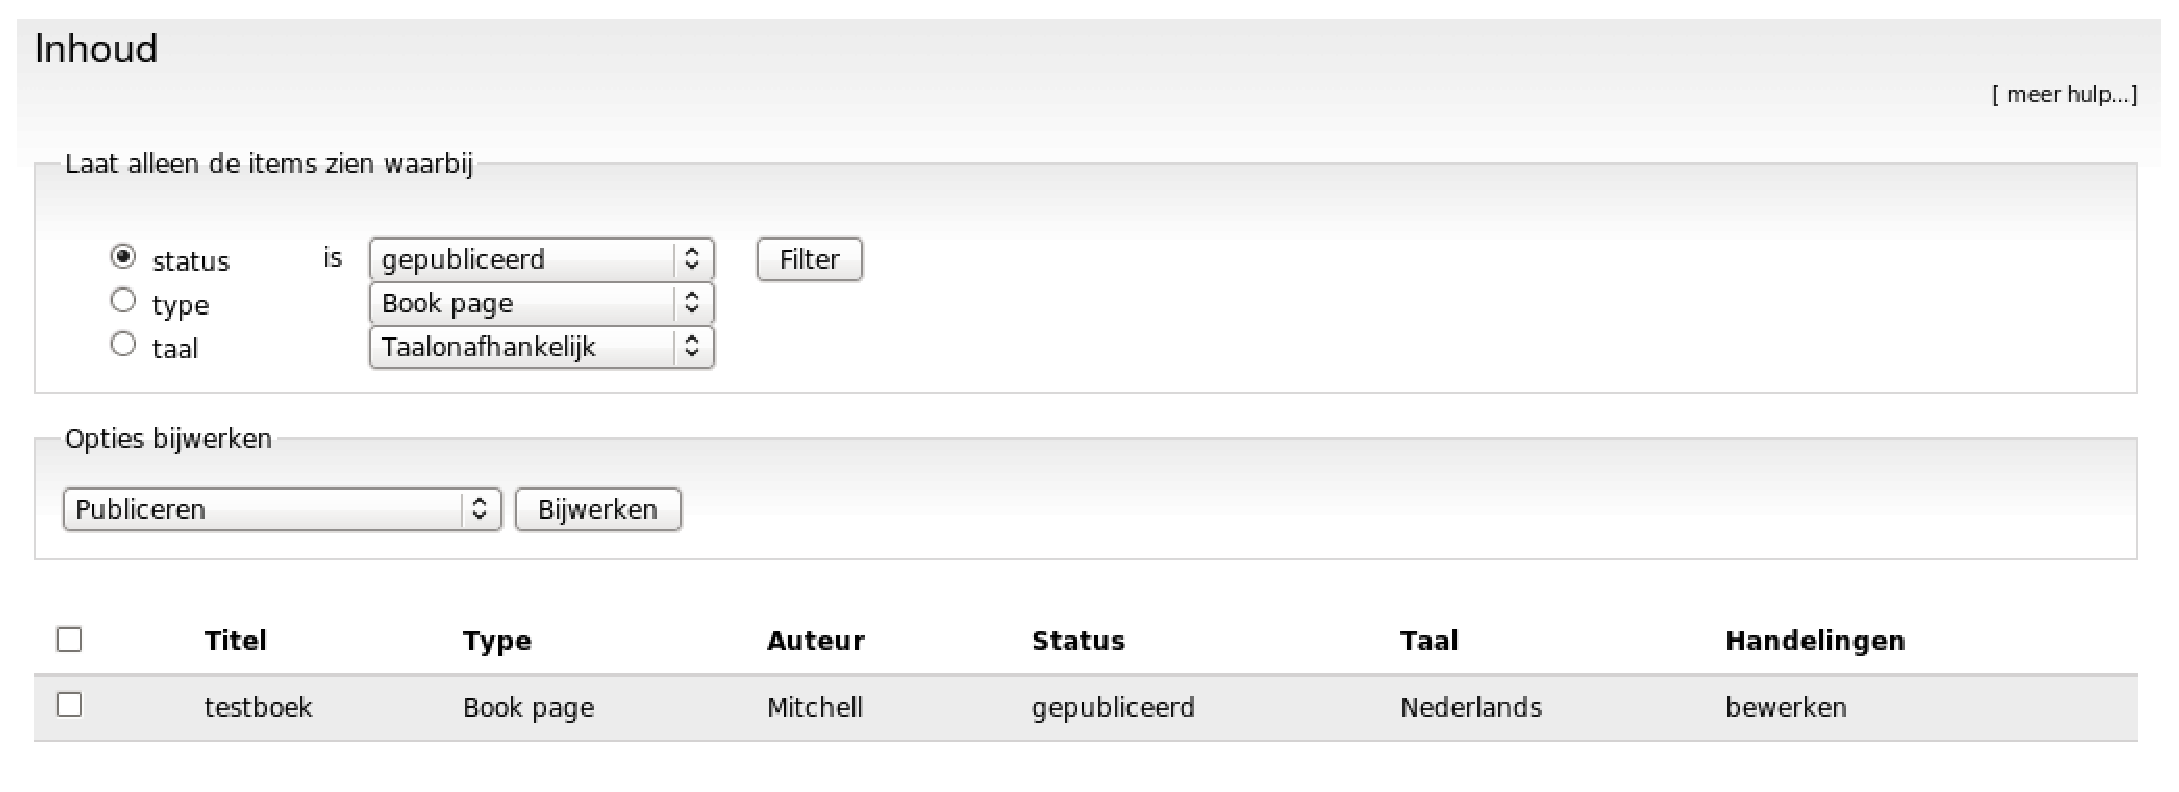
\includegraphics[scale=0.3,angle=0]{inhoud}
   \caption{Inhoud.\label{white}}
 \end{figure}
 \subsection{Node} \index{node}
De Node-module \index{node-module} beheert de inhoud van de site en slaat alle
ingevoerde pagina's (ongeacht het type) als 'node' op. De node bevat naast de publicatie opties (of een node gepubliceerd is, op de voorpagina zichtbaar is, bovenaan een
lijst wordt weergegeven) ook basisinformatie over de auteur van de pagina. Revisie-informatie van de node is
optioneel beschikbaar. Voor meer mogelijkheden wordt de Node-module vaak met andere modules uitgebreid.
\\
Iedere door gebruikers toegevoegde pagina op de website een node van een bepaald inhoudstype. Inhoudstypen
worden gebruikt om verschillende soorten pagina's of gegevenssoorten de defini\"eren. In een Inhoudstype zijn
eigenschappen vastgelegd zoals inclusief de paginatitel, type en aantal invoervelden en beschrijvingen bij de
invoervelden. Verder kunnen per inhoudstype verschillende standaard Publicatieopties en werkschema's worden ingesteld.
Standaard kent Drupal twee inhoudstypen: \index{inhoudstypen} Pagina
\index{pagina} en Verhaal \index{verhaal}. Op de pagina inhoudstypen kunnen
inhoudstypen worden toegevoegd. Ook kunnen typen worden toegevoegd door kern-modules, uitbreidingsmodules en zelf ontwikkelde modules.
\\
Op de pagina Inhoudelijk beheer vindt u een overzicht van de inhoud van de website en kunt u deze beheren.
De pagina Instellingen voor inzendingen bevat enkele instellingen voor de weergave van inzendingen.
De Node-module brengt voor ieder inhoudstype een aantal instellingen met zich mee die per rol op de
pagina Toegangsrechten kunnen worden ingesteld.

\section{Inhoudstypen}
Inzendingen per inhoudstype beheren zoals standaard status, aangeraden voor
voorpagina, enz.
\subsection{Lijst}
De onderstaande fig. geeft alle inhoudstypen op de site weer. Alle inzendingen
op de site zijn exemplaren van de onderstaande inhoudstypen.
 \begin{figure}[!h]
    \centering
   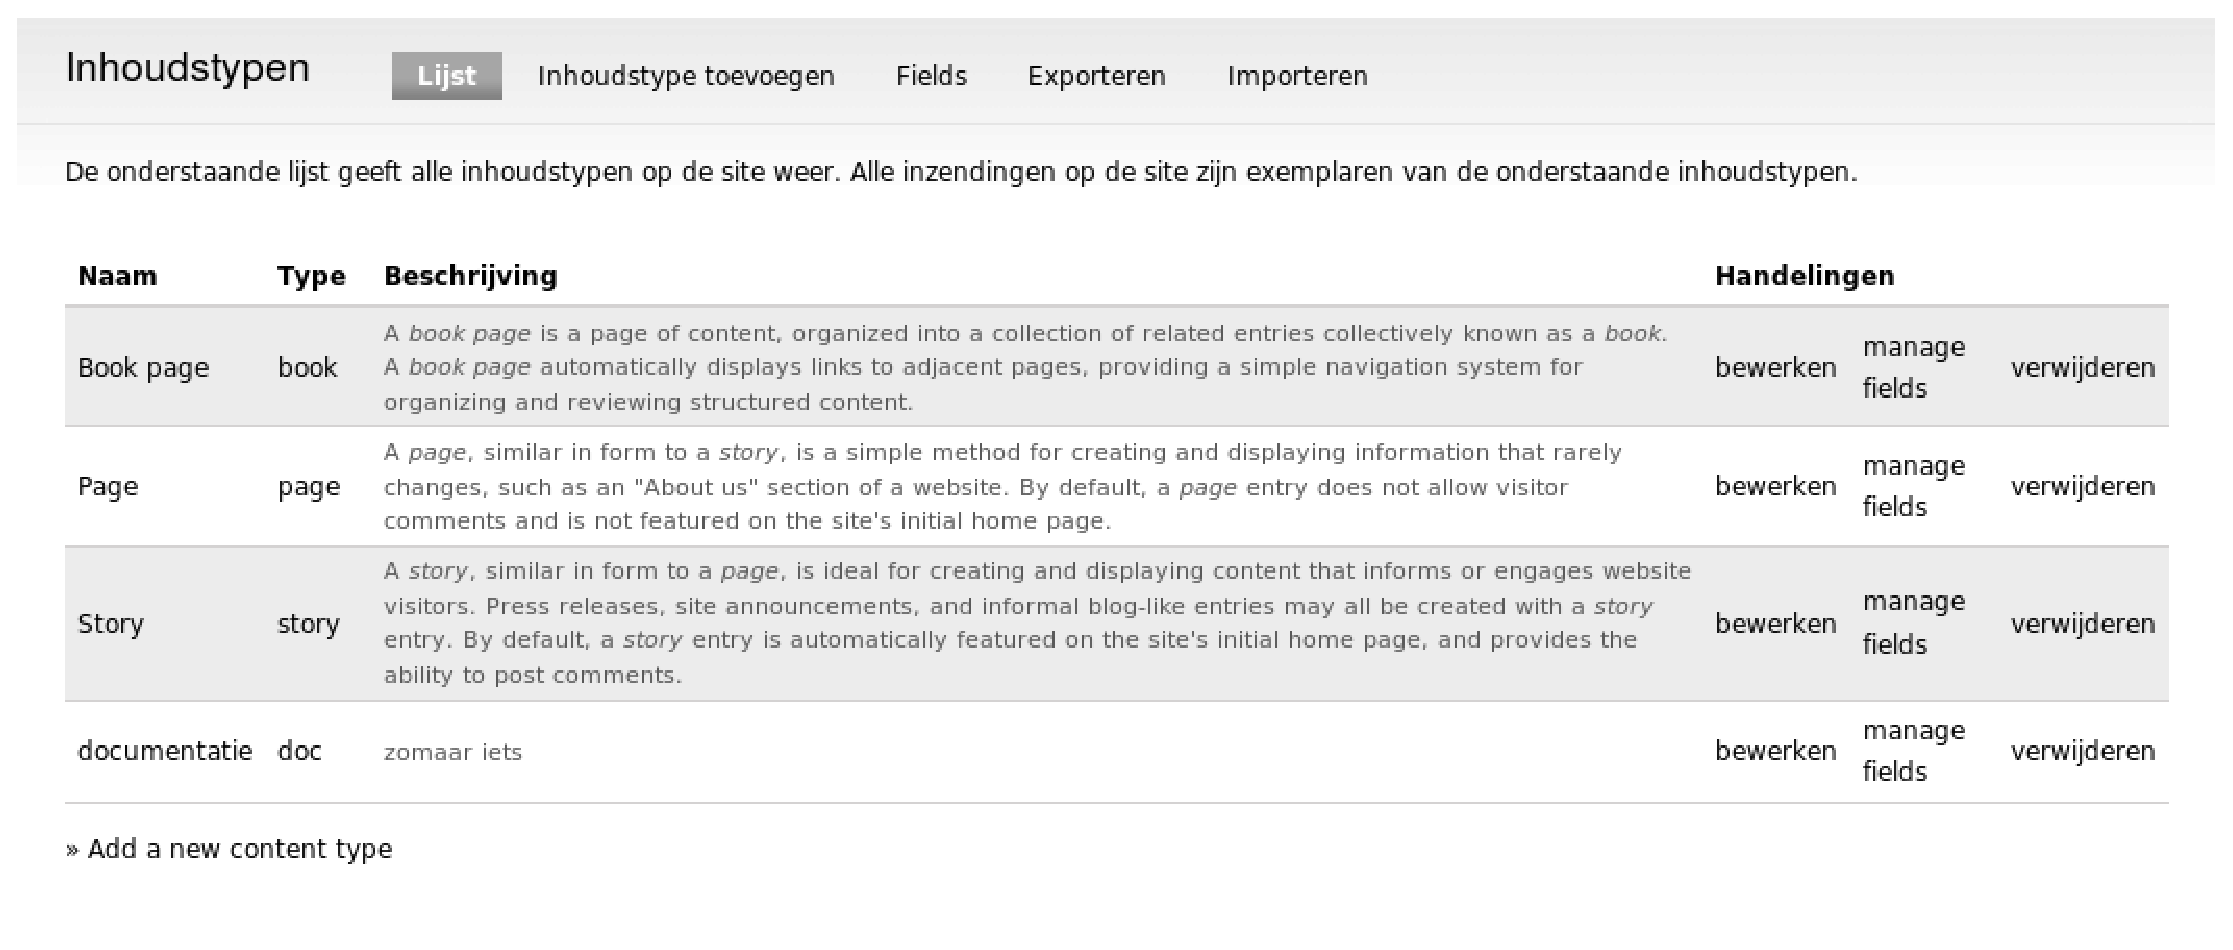
\includegraphics[scale=0.3,angle=0]{inhoudstypen-lijst}
   \caption{inhoudstypen-lijst.\label{white}}
 \end{figure}

\subsection{Inhoudstype toevoegen}
Maak een nieuw inhoudstype aan door een voor mensen begrijpelijke naam, een
machinaal leesbare naam en de overige relevante velden op deze pagina in te vullen.
Nadat een inhoudstype is aangemaakt kunnen gebruikers hiermee inhoud aan de site toevoegen.
\begin{figure}[!h]
    \centering
   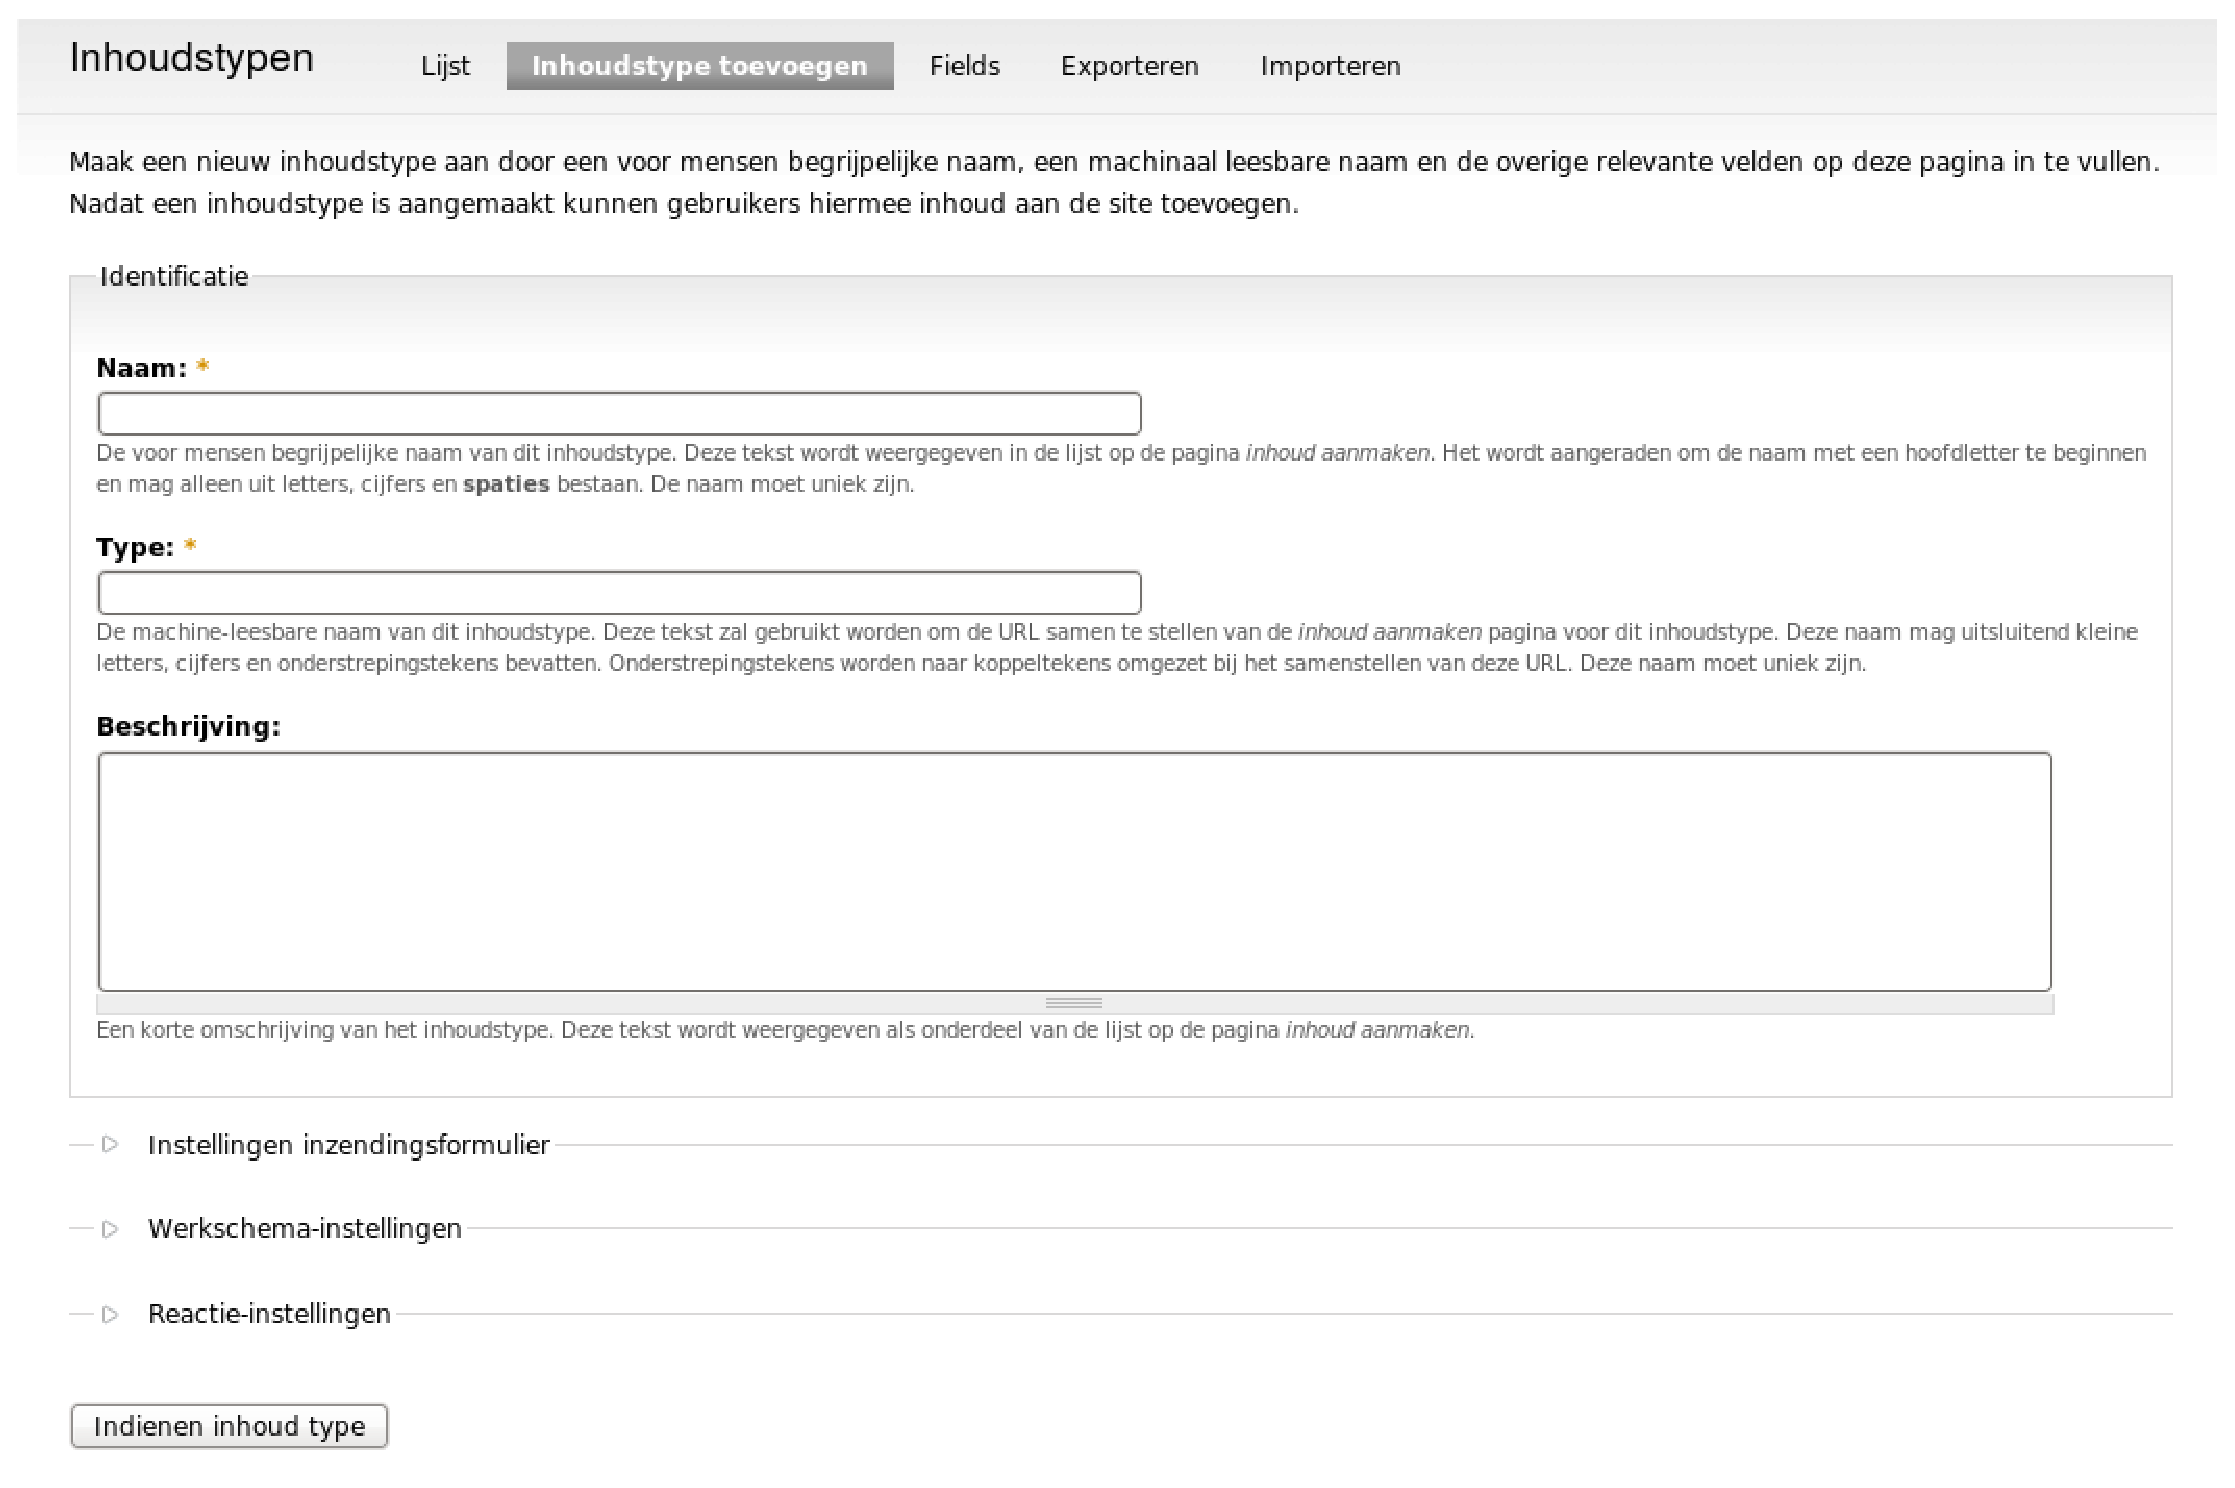
\includegraphics[scale=0.3,angle=0]{inhoudstypen-invoegen}
   \caption{inhoudstypen-invoegen.\label{white}}
 \end{figure}

\subsection{Fields}
\begin{figure}[!h]
    \centering
   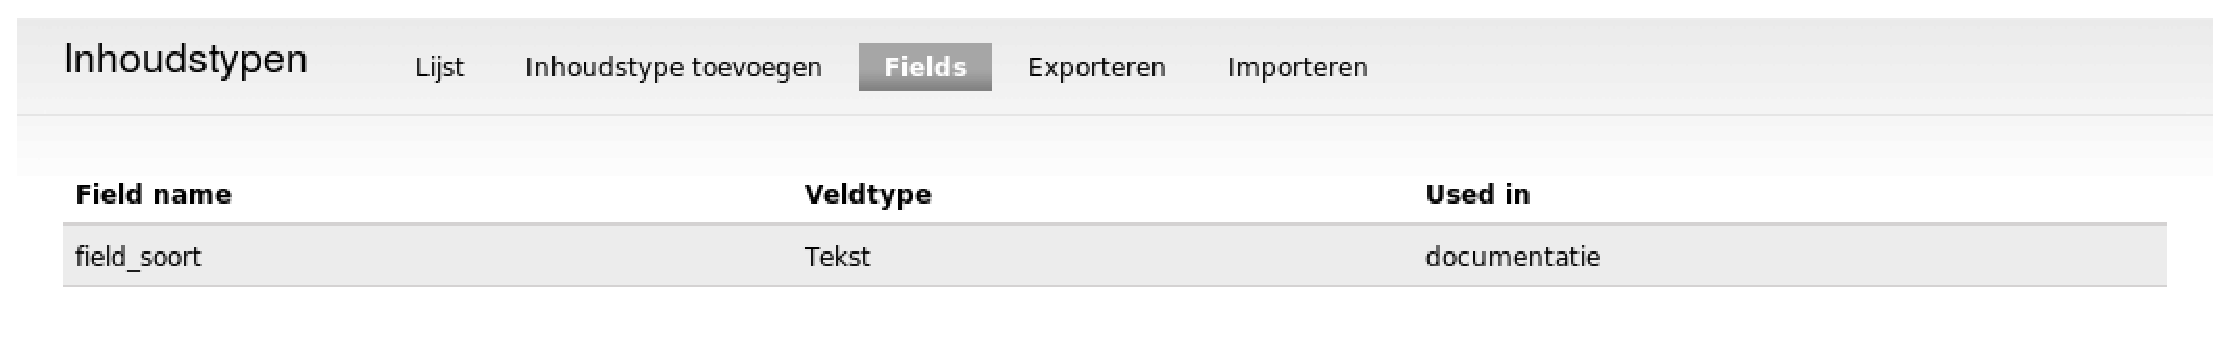
\includegraphics[scale=0.3,angle=0]{inhoudstypen-fields}
   \caption{inhoudstypen-fields.\label{white}}
 \end{figure}

\subsection{Exporteren} \index{exporteren}
This form will process a content type and one or more fields from that type and
export the settings. The export created by this process can be copied and pasted as
an import into the current or any other database. The import will add the fields to
an existing content type or create a new content type that includes the selected fields.
\begin{figure}[!h]
    \centering
   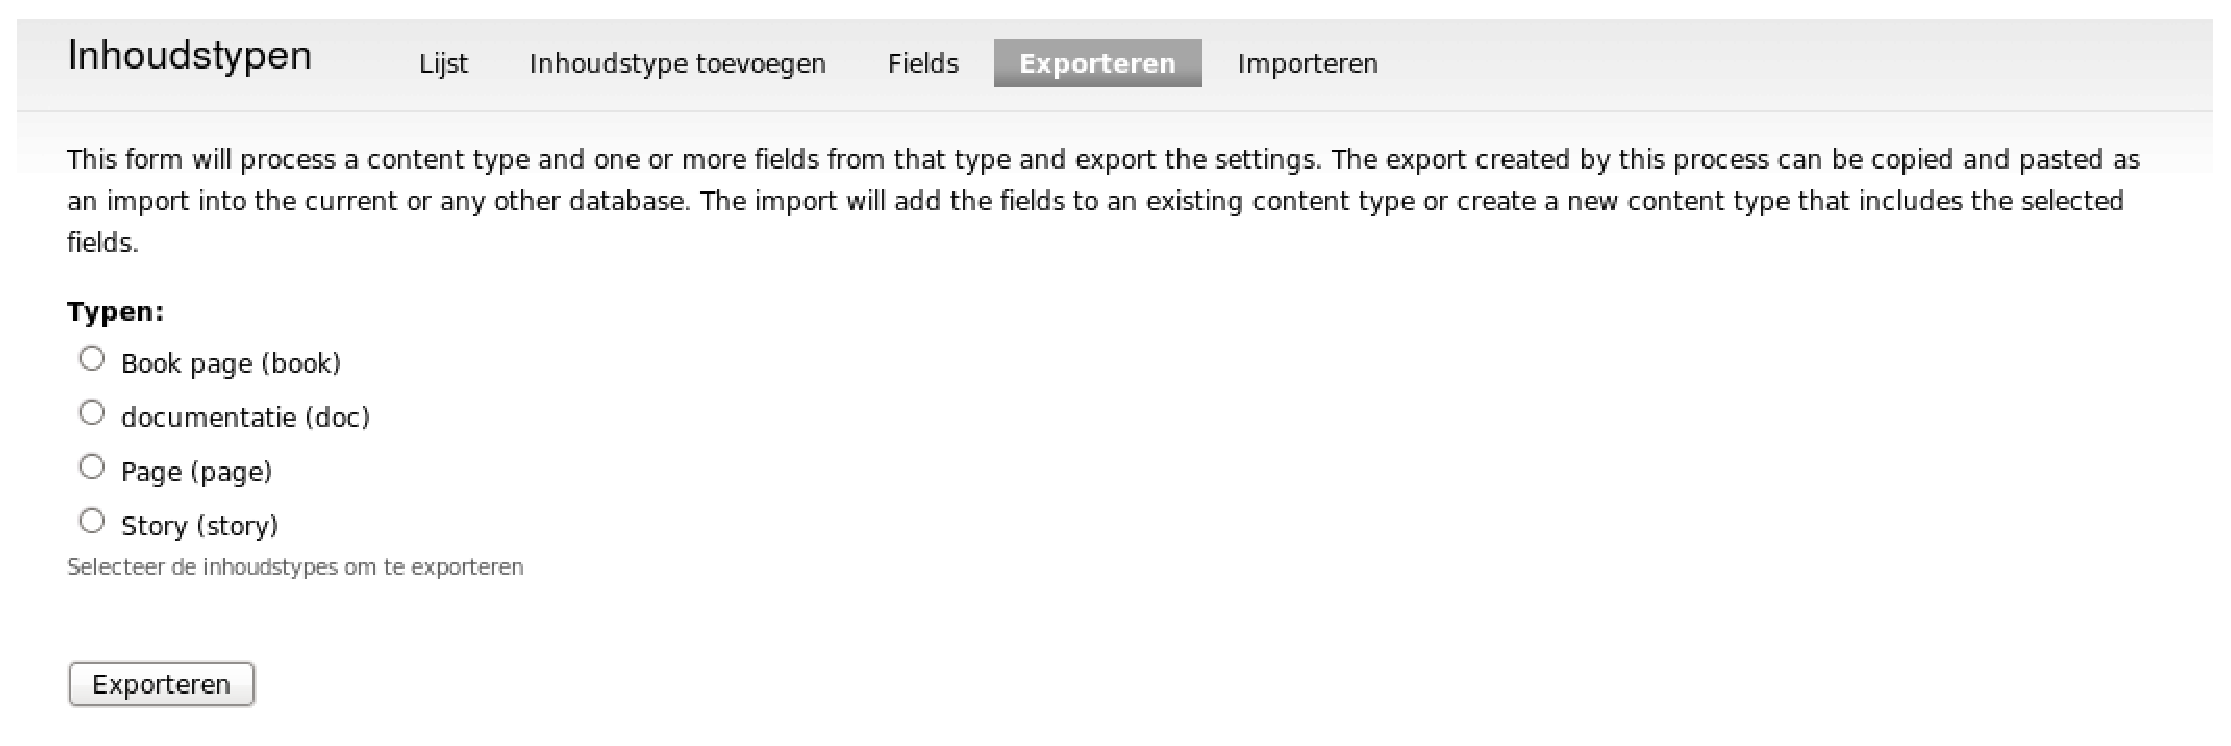
\includegraphics[scale=0.3,angle=0]{inhoudstypen-exporteren}
   \caption{inhoudstypen-exporteren.\label{white}}
 \end{figure}

\subsection{Importeren} \index{importeren}
Dit formulier zal veldinformatie importeren die zijn geexporteerd uit een ander inhoudstype of database.
Merk op dat velden niet kunnen worden gedupliceerd in hetzelfde inhoudstype, dus
ge\"importeerde velden zullen alleen worden toegevoegd als ze nog niet bestaan
in het geselecteerde inhoudstype. \begin{figure}[!h]
    \centering
   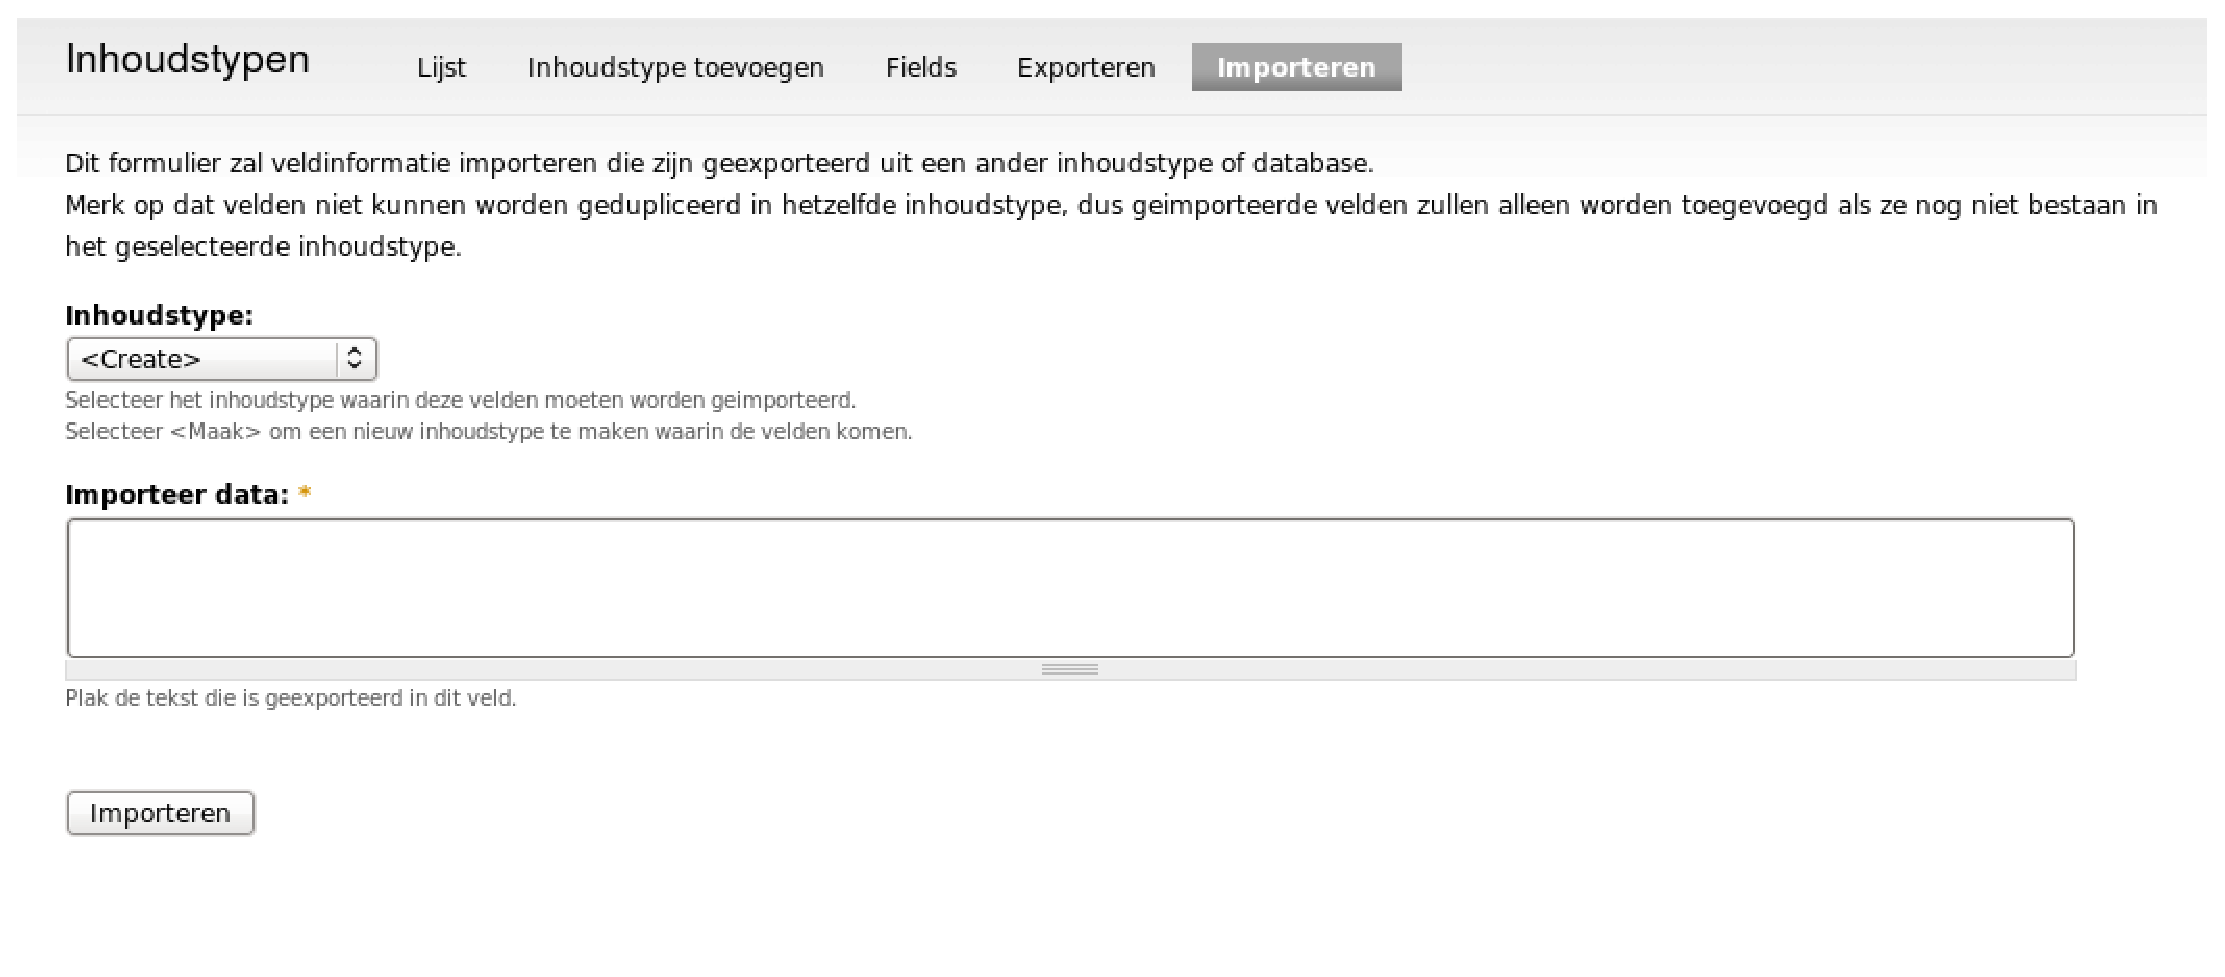
\includegraphics[scale=0.3,angle=0]{inhoudstypen-importeren}
   \caption{inhoudstypen-importeren.\label{white}}
 \end{figure}

\section{Instellingen voor inzendingen} \index{inzendingen}
Instellingen van inzendingen beheren zoals de lengte van het voorproefje,
verplichtte voorbeeldweergave \index{voorbeeldweergave} voor inzenden en het
aantal inzendingen op de voorpagina. \begin{figure}[!h]
    \centering
   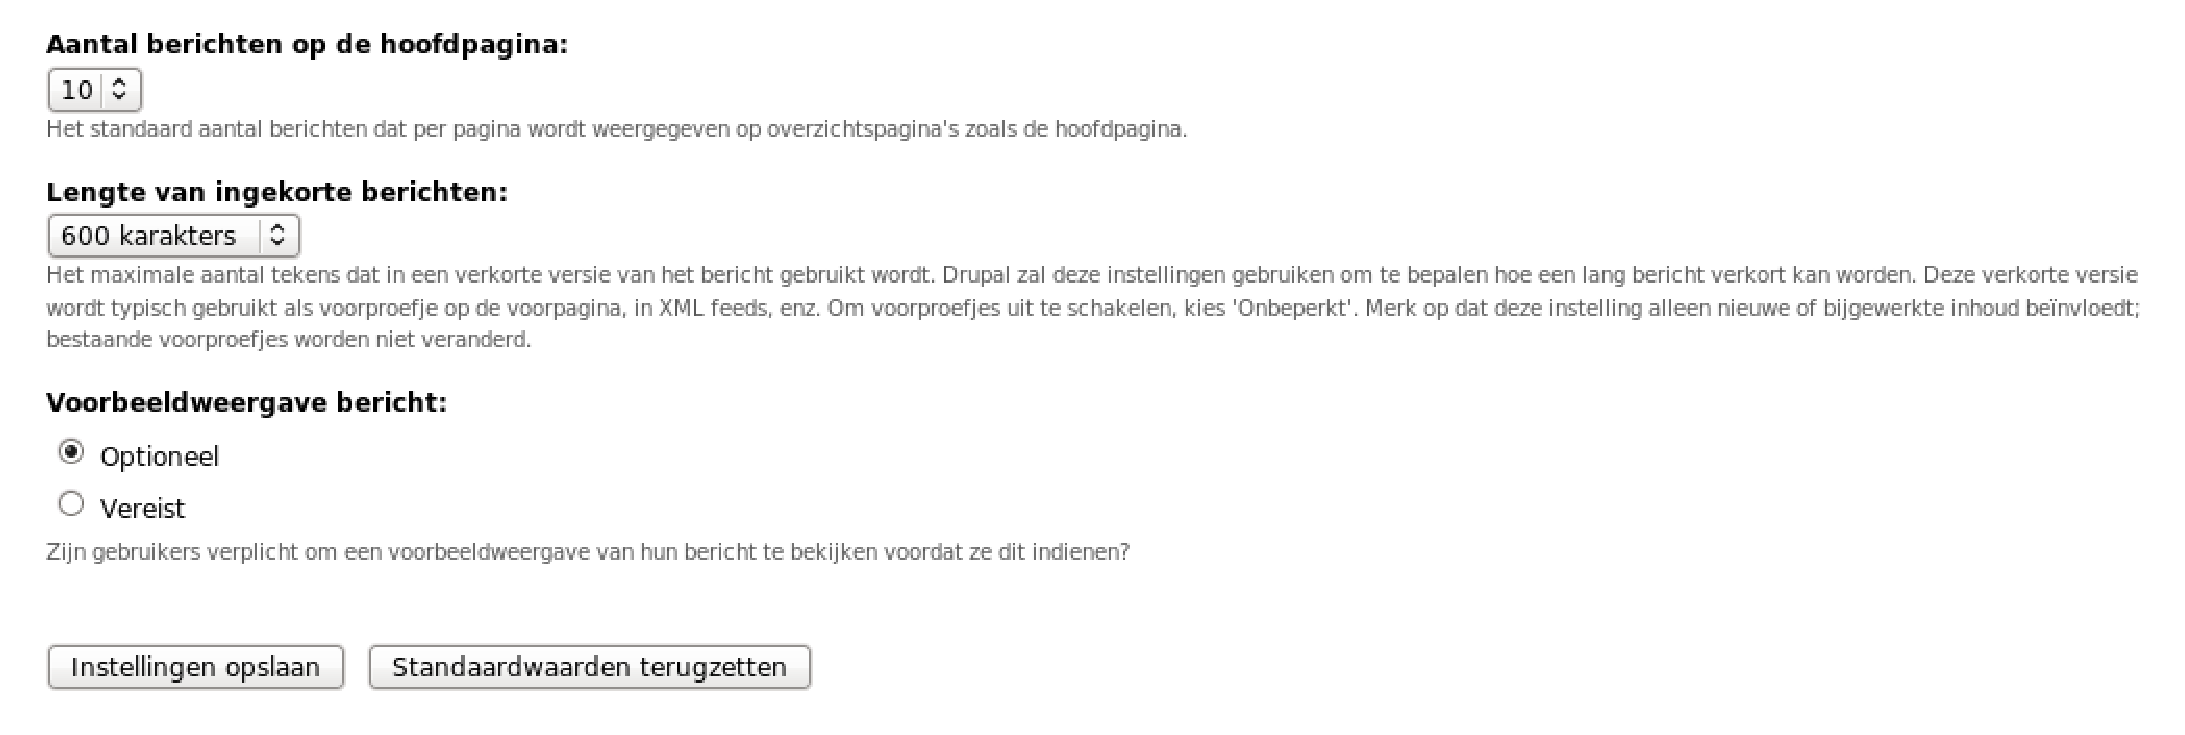
\includegraphics[scale=0.3,angle=0]{instellingen-inzendingen}
   \caption{instellingen-inzendingen.\label{white}}
 \end{figure}
\subsection{Node toegangsstatus} \index{toegangsstatus}
Wanneer er op de site problemen optreden met toegang tot de inhoud moet u de toegangsrechten-cache
opnieuw samenstellen. Mogelijke oorzaken voor toegangsproblemen zijn het uitschakelen van modules of
veranderingen in de toegangsrechten. Bij het opnieuw samenstellen van de cache worden alle rechten
verwijderd om te worden vervangen door rechten gebaseerd op actuele modules en instellingen.
\\
Het opnieuw samenstellen kan enige tijd in beslag nemen als de site veel inhoud bevat of als de
toegangsrechten complex zijn. Na afloop zullen alle berichten van de nieuwe toegangsrechten zijn voorzien.
\subsection{Aantal berichten op de hoofdpagina}
Het standaard aantal berichten dat per pagina wordt weergegeven op
overzichtspagina's zoals de hoofdpagina.
\subsection{Lengte van ingekorte berichten}
Het maximale aantal tekens dat in een verkorte versie van het bericht gebruikt
wordt. Drupal zal deze instellingen gebruiken om te bepalen hoe een lang bericht
verkort kan worden. Deze verkorte versie wordt typisch gebruikt als voorproefje op
de voorpagina, in XML feeds, enz. Om voorproefjes uit te schakelen, kies 'Onbeperkt'.
Merk op dat deze instelling alleen nieuwe of bijgewerkte inhoud be\"invloedt;
bestaande voorproefjes worden niet veranderd.
\subsection{Voorbeeldweergave bericht}
\begin{itemize}
\item Optioneel
\item Vereist
\end{itemize}
Zijn gebruikers verplicht om een voorbeeldweergave van hun bericht te bekijken
voordat ze dit indienen?

\section{RSS-publicatie} \index{rss-publicatie}
\begin{figure}[!h]
    \centering
   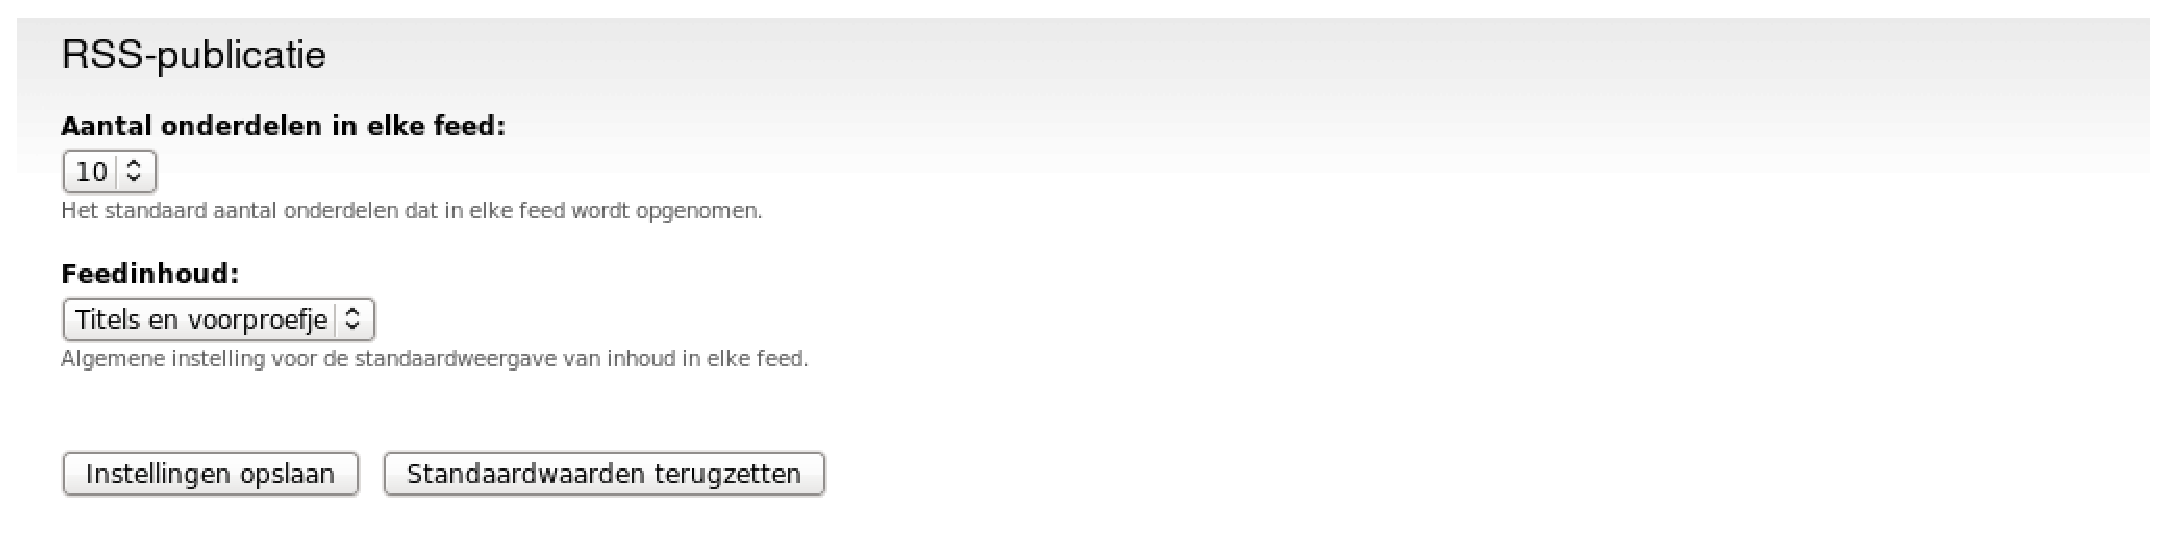
\includegraphics[scale=0.3,angle=0]{rss-publicatie}
   \caption{rss-publicatie.\label{white}}
 \end{figure}
Bepaal het aantal onderwerpen per feed en of feeds met titel, voorproefje of
volledige tekst worden weergegeven.

\section{Reacties} \index{reacties}
Reacties en de moderatiewachtrij voor reacties weergeven en wijzigen.
\subsection{Comment-module} \index{comment-module}
Met de Comment-module kunnen bezoekers reageren op uw bijdrage in een ad-hoc discussieforum.
Ieder inhoudstype kan Standaard reactie-instellingen hebben voor Lezen/Schrijven van een reactie
of de mogelijkheid tot reageren is Uitgeschakeld. Instellingen voor weergave van reacties en andere
reactie-instellingen kunnen ook per nodetype worden bepaald. Sommige weergave-instellingen zijn per gebruiker te bepalen.
\\
Reactierechten \index{reactierechten} worden toegekend per gebruikersrol en
worden gebruikt om te bepalen of anonieme bezoekers of gebruikers met andere rollen het recht hebben op een inzending te reageren. Als anonieme bezoekers het
recht hebben om te reageren, kan contactinformatie in een cookie op de computer van de bezoeker worden
opgeslagen voor gebruik bij volgende reacties. Als er geen vervolg-reacties zijn op een reactie kan de
auteur (optioneel) de eigen reactie wijzigen. De Comment-module gebruikt de zelfde invoerformaten en
HTML-tags als bij het aanmaken van andere inhoud beschikbaar zijn.
\subsection{Gepubliceerde reacties} \index{gepubliceerde reacties}
Een lijst van recente reacties op de site. Klik op het onderwerp om de reactie
te lezen, op de naam van de schrijver om de gebruikersinformatie van de schrijver
te bewerken, op 'bewerken' om de tekst te bewerken of op 'verwijderen' om de reactie te verwijderen.
\begin{figure}[!h]
    \centering
   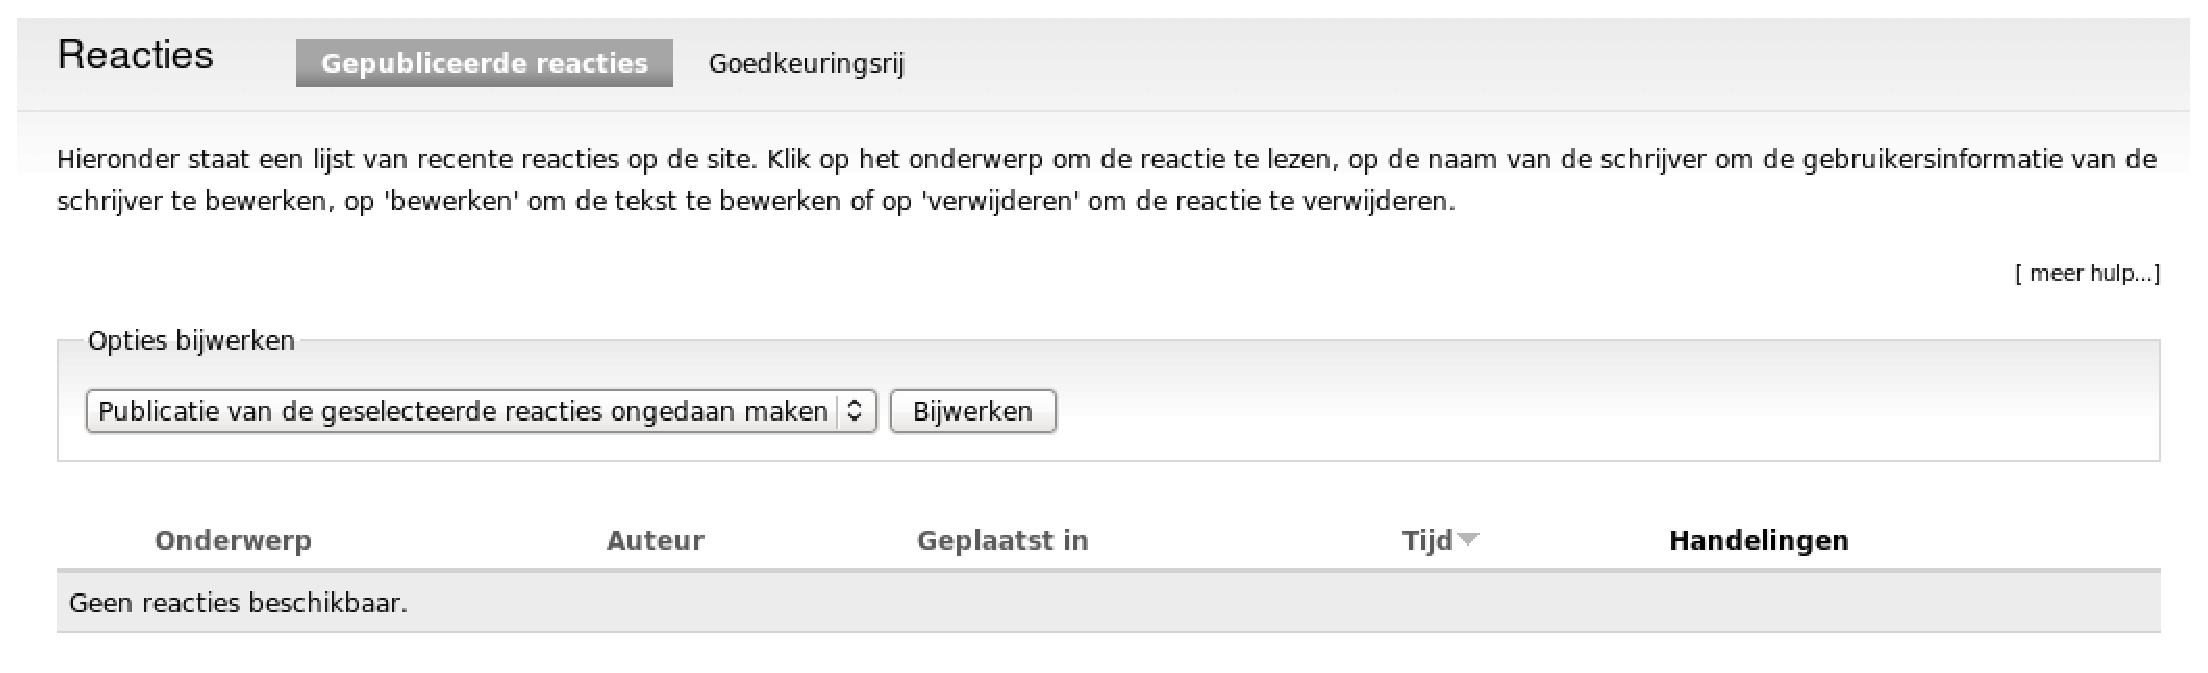
\includegraphics[scale=0.3,angle=0]{reacties-geplubliceerd}
   \caption{reacties-geplubliceerd.\label{white}}
 \end{figure}
\subsection{Goedkeuringsrij} \index{goedkeuringsrij}
Een lijst van recente reacties die moeten worden goedgekeurd. Klik op
'bewerken' en wijzig de 'moderatiestatus' \index{moderatiestatus} in Goedgekeurd
om een reactie goed te keuren. Klik op een onderwerp om de reactie te zien, op de naam van de schrijver om de gebruikersinformatie
te bewerken, op 'bewerken' om de tekst te bewerken en op 'verwijderen' om de
reactie te verwijderen. \begin{figure}[!h]
    \centering
   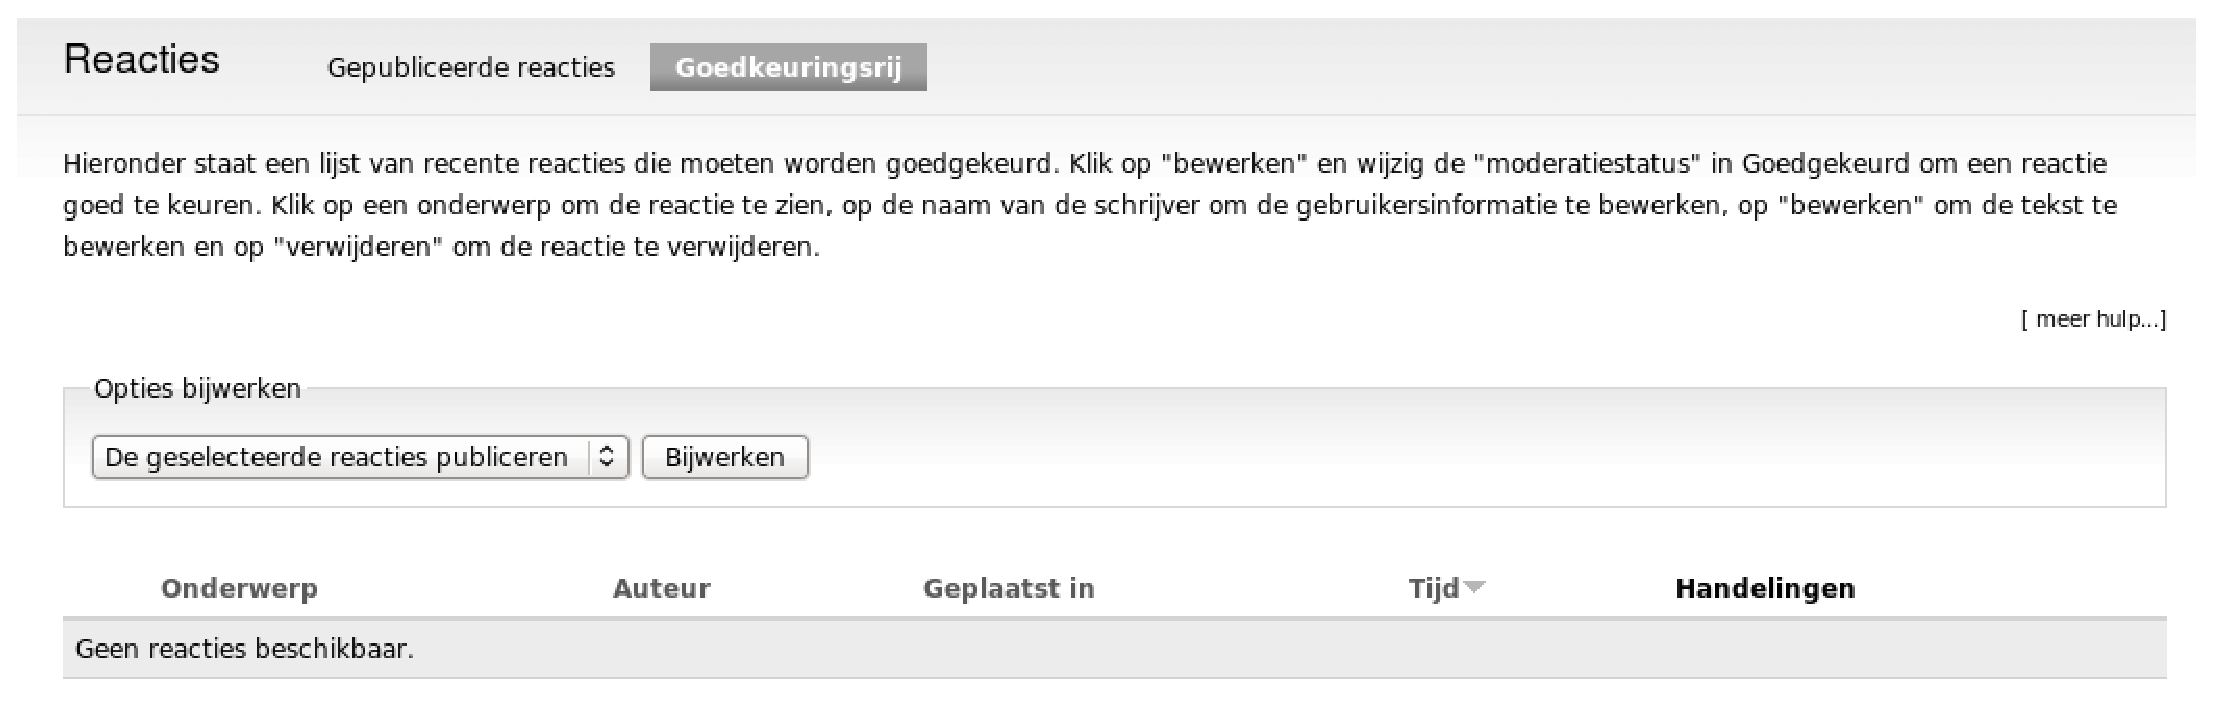
\includegraphics[scale=0.3,angle=0]{reacties-goedkeuringsrij}
   \caption{reacties-goedkeuringsrij.\label{white}}
 \end{figure}

\section{Taxonomie} \index{taxonomie}
Beheren van labelen \index{labelen}, categoriseren \index{categoriseren} en
classificeren \index{classificeren} van de website-inhoud.
\subparagraph{Taxonomy-module} \index{taxonomie-module}
Met de Taxonomy-module kunt u de inhoud van de website met behulp van verschillende
classificatie systemen categoriseren. Met 'Vrij labelen' kunnen gebruikers tijdens het
indienen van inhoud deze van zelf gekozen labels voorzien (deze methode wordt vaak in
blogs en community-sites toegepast). Met gecontroleerde woordenlijsten kunnen eenvoudige
lijsten, maar ook complexe hi\"erarchie\"en met meervoudige relaties tussen de termen, worden
samengesteld om inhoud te categoriseren. Deze methoden kunnen op verschilende inhoudstypen
worden toegepast en gecombineerd worden tot een krachtige en flexibele methode voor het
classificeren en presenteren van de website-inhoud.
\\
Wanneer u bijvoorbeeld een receptensite maakt, wilt u wellicht berichten classificeren op het
soort maaltijd en op bereidingstijd. Met een woordenlijst voor maaltijd \'en
voor bereidingstijd kunt u beide criteria onafhankelijk van elkaar gebruiken in plaats van voor elke mogelijke combinatie een nieuwe label aan te maken.
\begin{itemize}
\item Soort gerecht: Voorgerecht, Hoofdgerecht, Salade, Dessert
\item Bereidingstijd: 0-30 min., 30-60 min., 1-2 uur, meer dan 2 uur
\end{itemize}
Iedere taxonomie-term (in andere systemen ook wel 'categorie' of 'tag' genoemd) voorziet standaard
in een lijst van inzendingen met deze term en een bijbehorende RSS-feed. De URL's van deze lijsten
kunnen worden samengesteld om EN- en OF-lijsten te maken van inzendingen die van verschillende termen
zijn voorzien. In het voorbeeld van de receptensite kunnen eenvoudig pagina's gemaakt worden met alle
'Hoofdgerechten', '30 minuten' recepten of een samengestelde lijst '30 minuten hoofdgerechten en voorgerechten'
door gebruik te maken van losse of gecombineerde termen. Er is een groot aantal uitbreidingsmodules beschikbaar
waarmee u de functionaliteit van de kernmodules op het gebied van weergave en organisatie van termen kunt veranderen en uitbreiden.
\\
Op de beheerpagina kunnen termen hi\"erarchisch gerangschikt worden. Bijvoorbeeld landen rangschikken van onder regio's in de wereld.
Met de Taxonomy-module kunnen gegevens op geavanceerde wijze worden gerangschikt. Zoals bijvoorbeeld Turkije plaatsen onder
'Midden Oosten' \'en onder 'Europa'.
\\
De Taxonomy-module maakt het gebruik van synoniemen en gerelateerde termen mogelijk maar kent geen actieve ondersteuning hiervan.
Uitbreidingsmodules kunnen deze functies echter volledig benutten.
\subsection{Lijst}
Met de Taxonomy-module kunt u inhoud van de site classificeren met labels en
gecontroleerde termen. Het is een flexibel classificatie gereedschap met geavanceerde mogelijkheden.
Om te beginnen wordt een 'Woordenlijst' aangemaakt voor een groep van labels of termen.
U kunt één woordenlijst voor vrij-labelen voor alle termen aanmaken of verschillende gecontroleerde
woordenlijsten die ieder verschillende eigenschappen van de inhoud weergeven; Bijvoorbeeld: 'Landen' en 'Kleuren'.
\\
De onderstaande lijst kan gebruikt worden om de gebruikte woordenlijsten te controleren
en te configureren of om de termen (labels) daarin te beheren. Een woordenlijst is (optioneel)
gekoppeld aan een inhoudstype weergegeven in de kolom Type en wordt bij het aanmaken of bewerken
van een pagina van dit inhoudstype weergegeven. Wanneer meerdere woordenlijsten aan een zelfde
inhoudstype zijn gekoppeld worden deze in de onderstaande volgorde weergegeven. Om de volgorde
van de woordenlijsten aan te passen klik-sleept u een woordenlijst aan het handvat in de kolom
Naam naar een nieuwe positie in de lijst. (U klik-sleept het blok door met de muis boven het
handvatpictogram te klikken, vast te houden en de muis te verplaatsen.) Wijzigingen worden
pas opgeslagen wanneer u de knop Opslaan onderaan de pagina aanklikt.
\subsection{Woordenlijst toevoegen} \index{woordenlijst toevoegen}
\begin{figure}[!h]
    \centering
   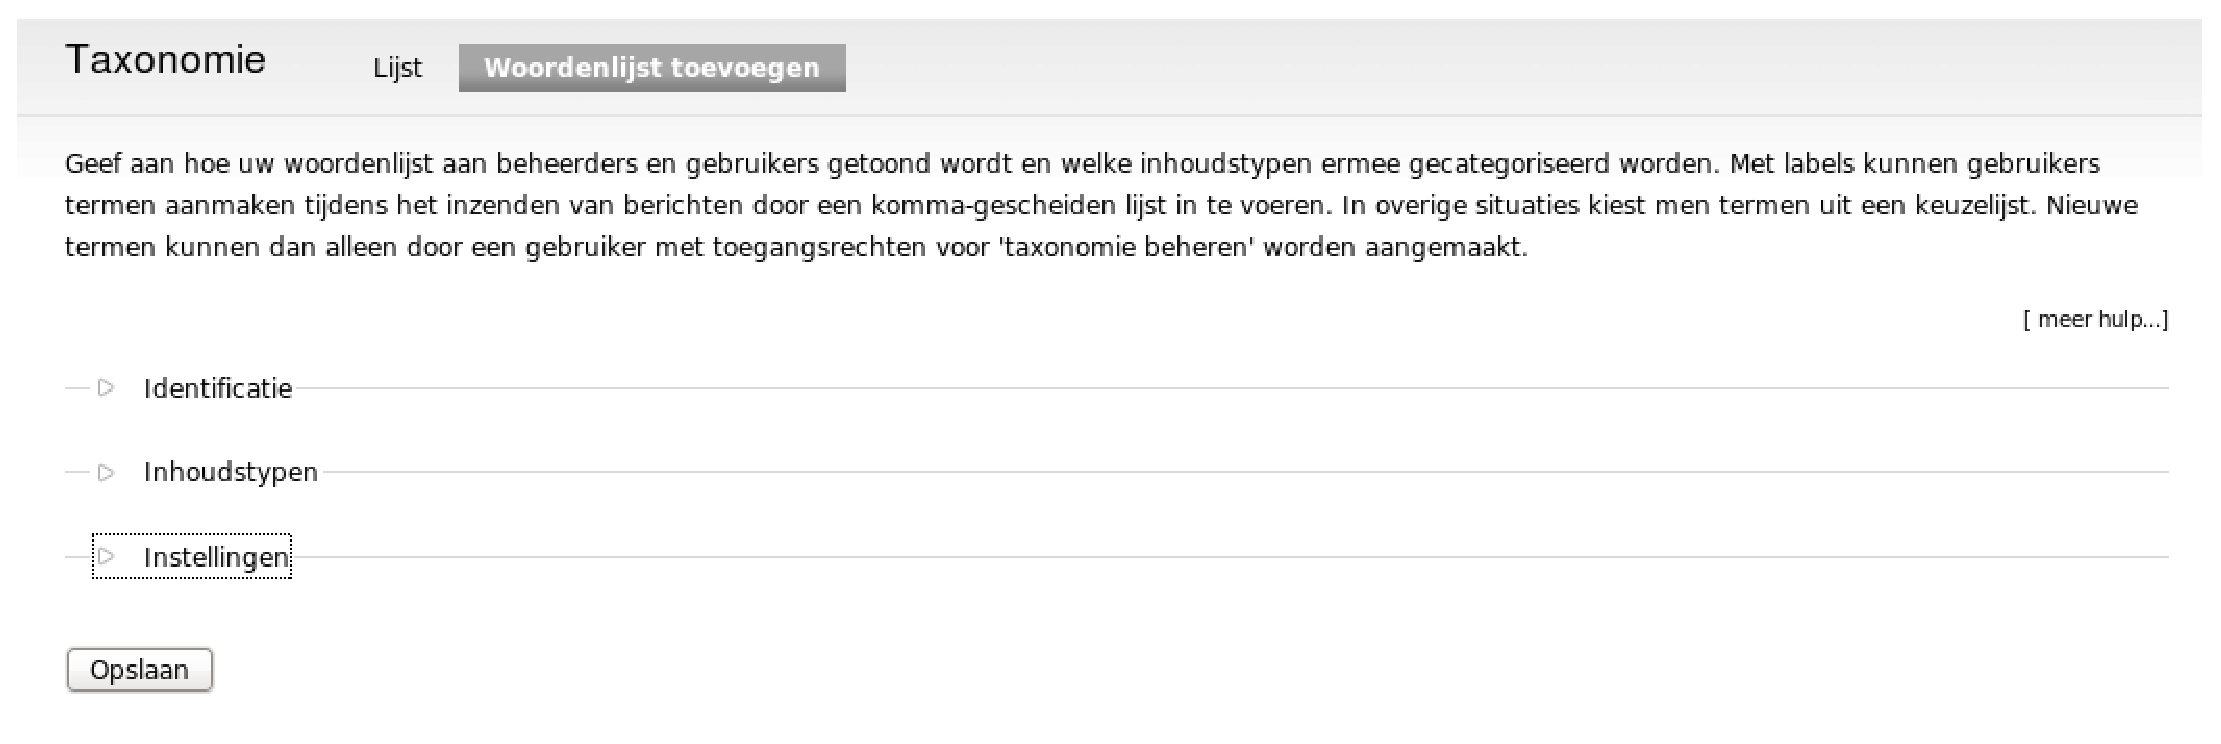
\includegraphics[scale=0.3,angle=0]{woordenlijst-toevoegen}
   \caption{woordenlijst-toevoegen.\label{white}}
 \end{figure}
Geef aan hoe uw woordenlijst aan beheerders en gebruikers getoond wordt en welke
inhoudstypen ermee gecategoriseerd worden. Met labels kunnen gebruikers termen aanmaken
tijdens het inzenden van berichten door een komma-gescheiden lijst in te voeren.
In overige situaties kiest men termen uit een keuzelijst. Nieuwe termen kunnen dan
alleen door een gebruiker met toegangsrechten voor 'taxonomie beheren' worden aangemaakt.
\subsubsection{Woordenlijst-identificatie} \index{identificatie woordenlijst}
\begin{itemize}
\item Naam van woordenlijst: De naam van deze woordenlijst. Bijvoorbeeld:''tags''
\item Beschrijving: Beschrijving van de woordenlijst; kan gebruikt worden door
modules.
\item Helptekst: Instructies voor de gebruiker bij het selecteren van termen.
Bijvoorbeeld: ''Voer een lijst in, gescheiden door komma's''.
\end{itemize}
\begin{figure}[!h]
    \centering
   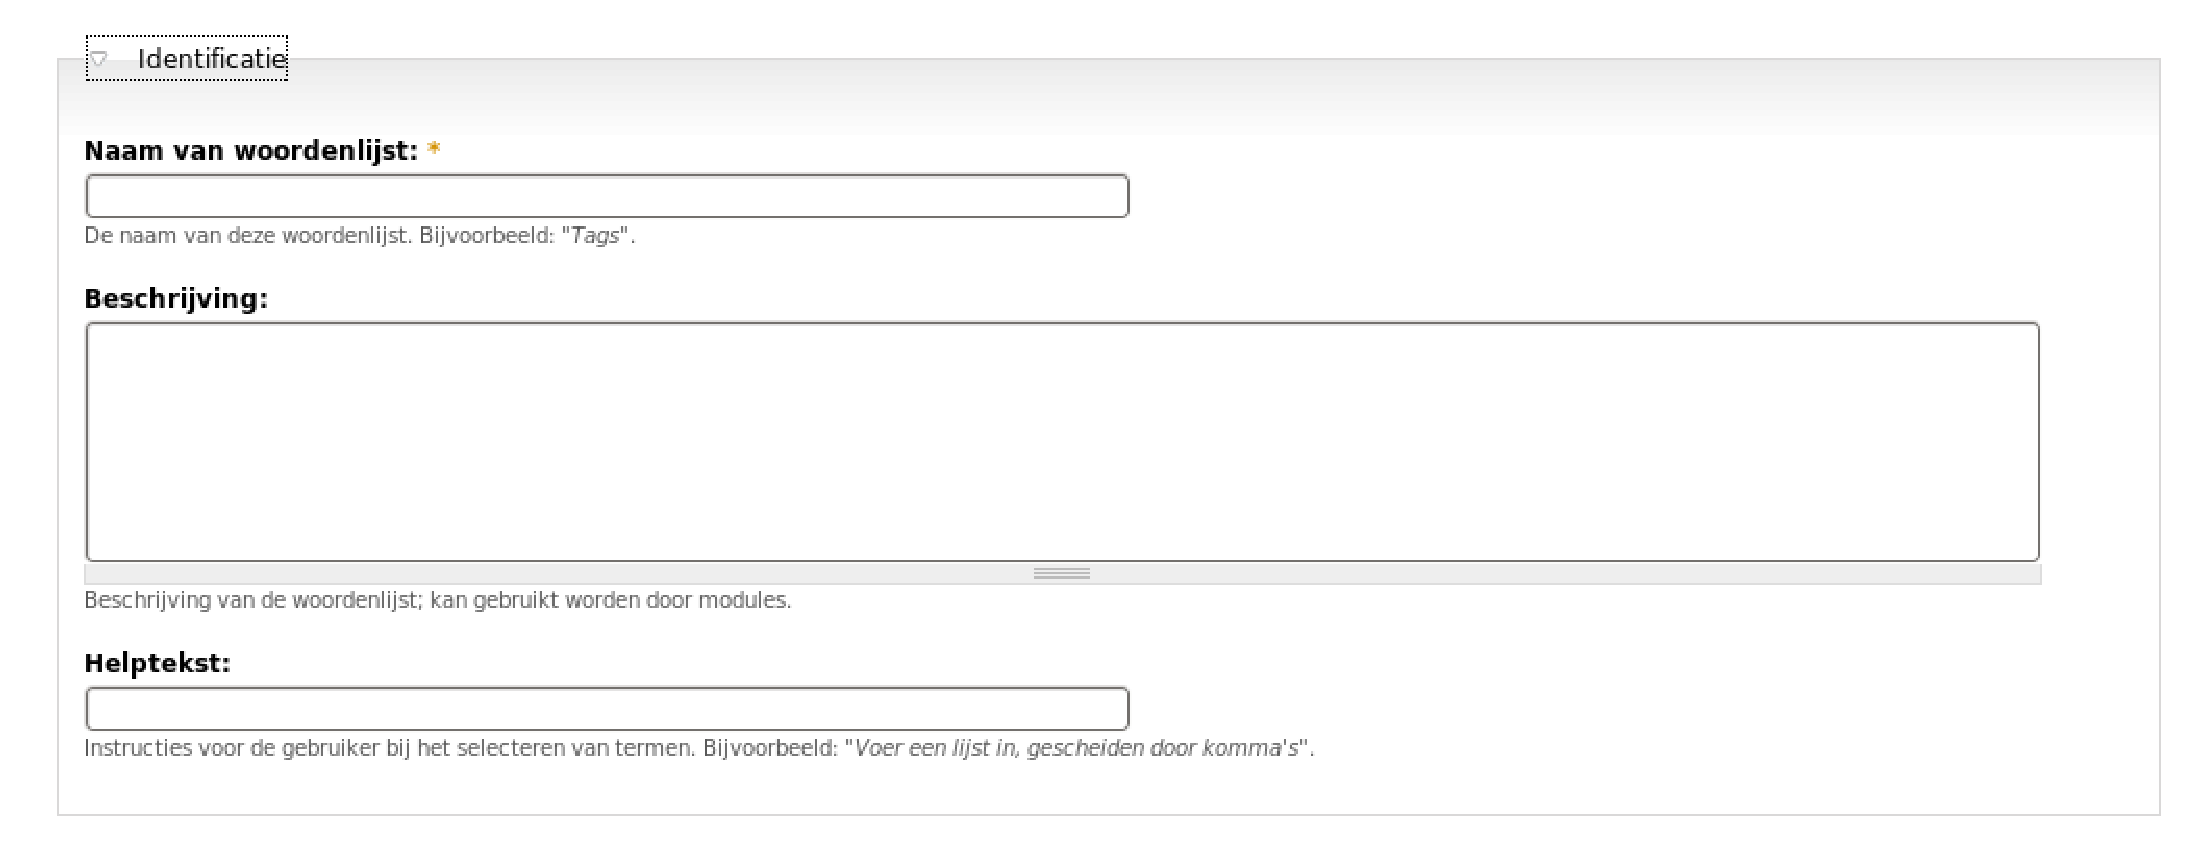
\includegraphics[scale=0.3,angle=0]{woordenlijst-identificatie}
   \caption{Woordenlijst-identificatie.\label{white}}
 \end{figure}
 \subsubsection{Woordenlijst-inhoudstypen}
 Gebruik de woordenlijst om inhoudstypen te categoriseren.
\begin{itemize}
\item Book page
\item Page
\item Story
\item \ldots
\end{itemize}
\begin{figure}[!h]
    \centering
   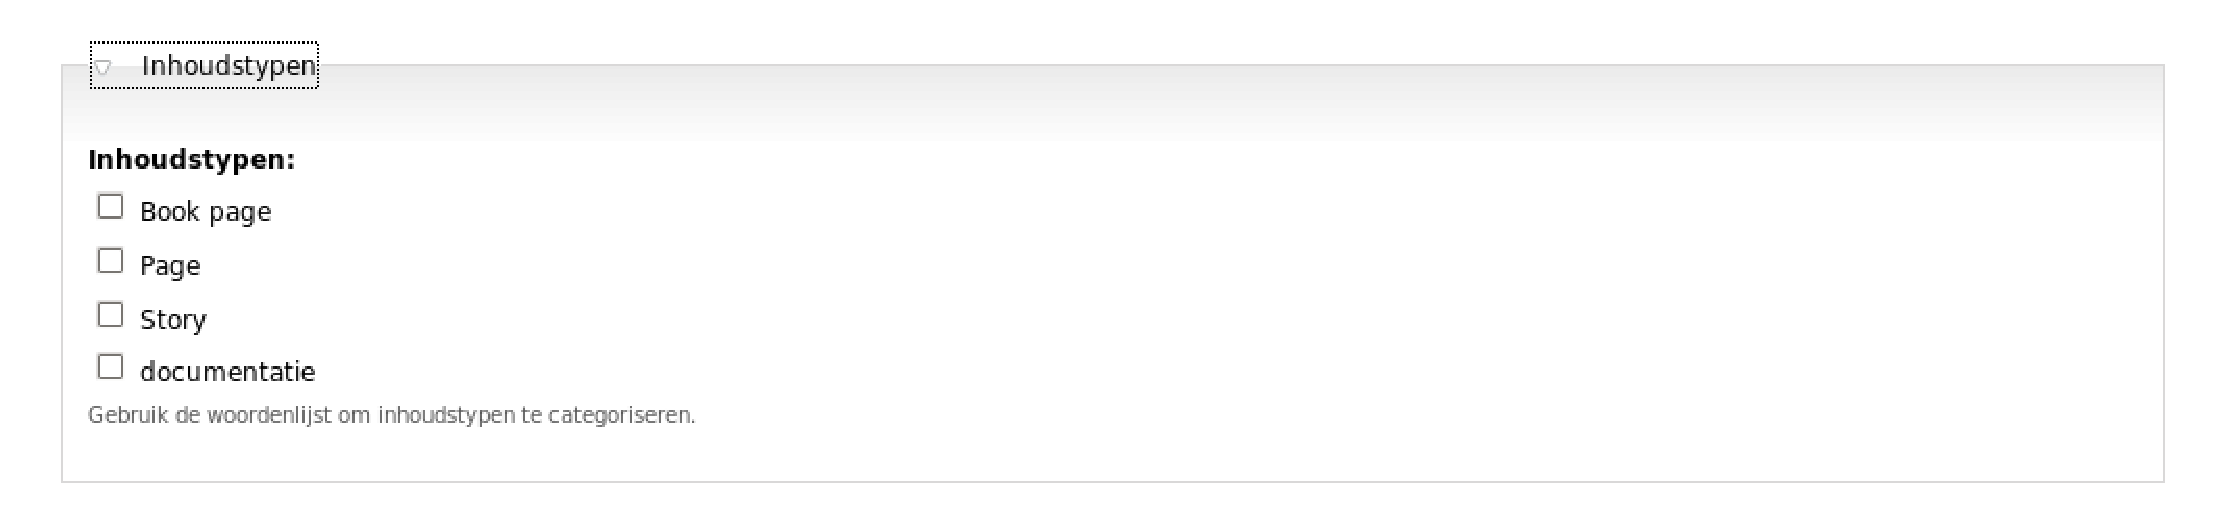
\includegraphics[scale=0.3,angle=0]{woordenlijst-inhoudstypen}
   \caption{woordenlijst-inhoudstypen.\label{white}}
 \end{figure}

 \subsubsection{Woordenlijst-instellingen} \index{instellingen woordenlijst}
 \begin{itemize}
\item Labels: Termen worden aangemaakt wanneer gebruikers een door komma's
gescheiden lijst indienen.
\item Meervoudige selectie: Inzendingen mogen meer dan \'e\'en term uit deze
woordenlijst bevatten (altijd geldig voor labels).
\item Vereist: Inzendingen moeten minimaal \'e\'en term uit deze woordenlijst
bevatten.
\end{itemize}
\begin{figure}[!h]
    \centering
   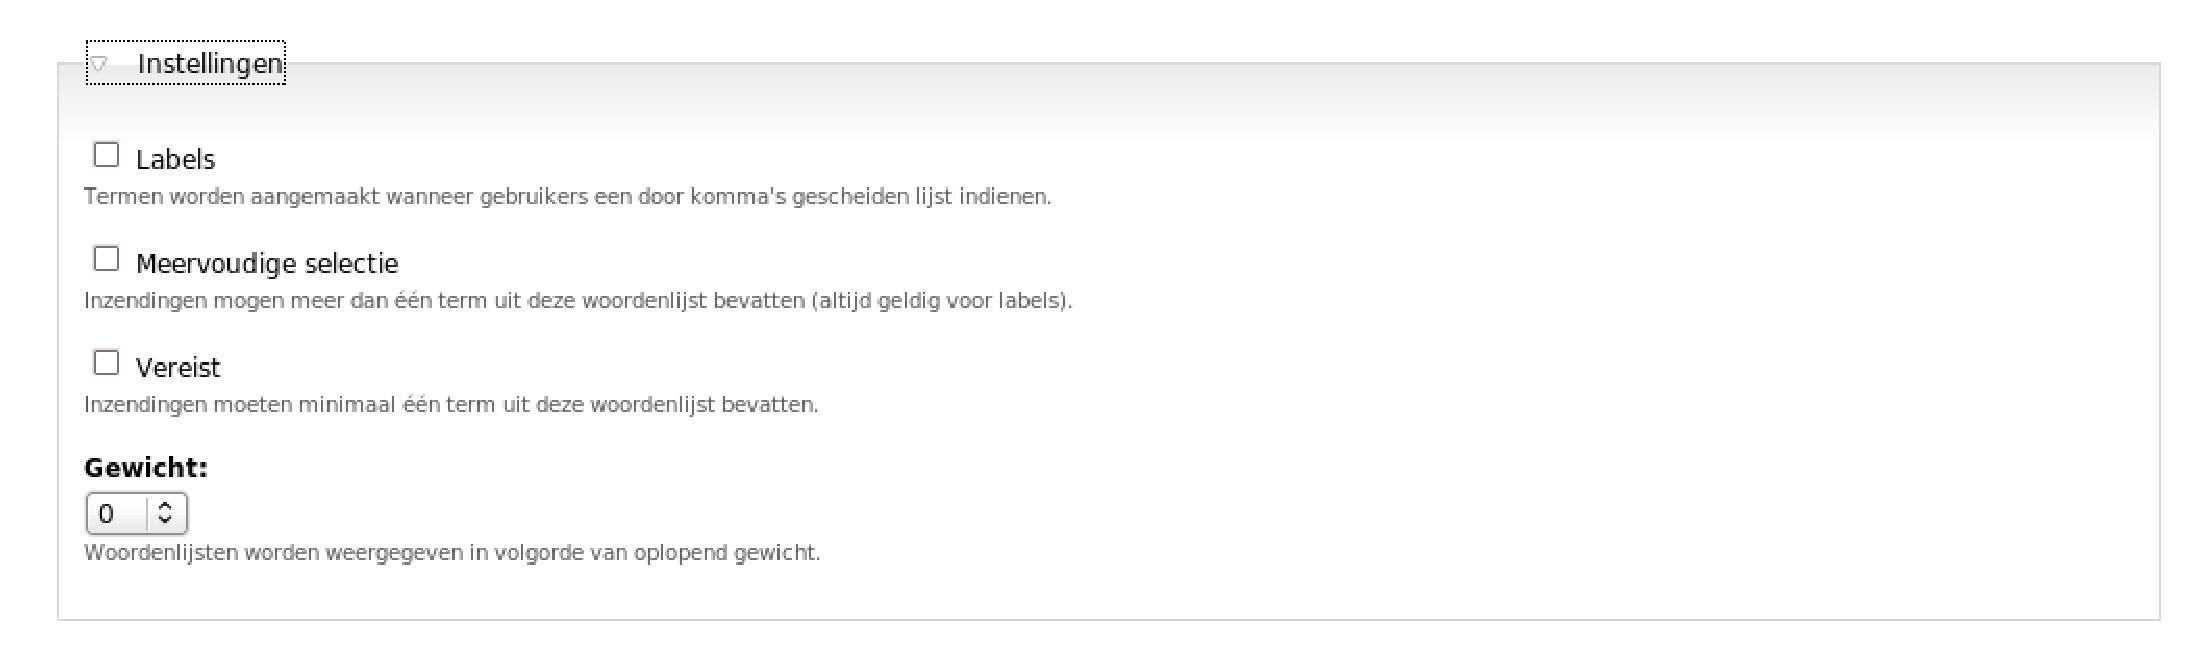
\includegraphics[scale=0.3,angle=0]{woordenlijst-instellingen}
   \caption{Woordenlijst-instellingen.\label{white}}
 \end{figure}
 blabla
%  \chapter{Site-constructie} \index{site-constructie}
\section{Blokken}
Bepalen welke blokken in de zijbalken of in een ander gebied van de pagina
worden weergegeven.
\subsection{Blokkenlijst} \index{blokkenlijst}
Op deze pagina kan u door middel van slepen en neerzetten een blok in een gebied
plaatsen en de volgorde van blokken binnen het gebied wijzigen. Om een blok te verplaatsen 
klik-sleept u het blok aan het handvat in de kolom Blok naar een nieuwe positie in de lijst. 
(U klik-sleept het blok door met de muis boven het handvatpictogram te klikken, vast te houden 
en de muis te verplaatsen.) Omdat niet alle templates de zelfde gebieden gebruiken of gebieden 
op de zelfde manier weergeven, worden blokposities per template bepaald. Wijzigingen worden 
pas opgeslagen wanneer u de knop Blok opslaan onderaan de pagina aanklikt.
\begin{figure}[!h]
    \centering
   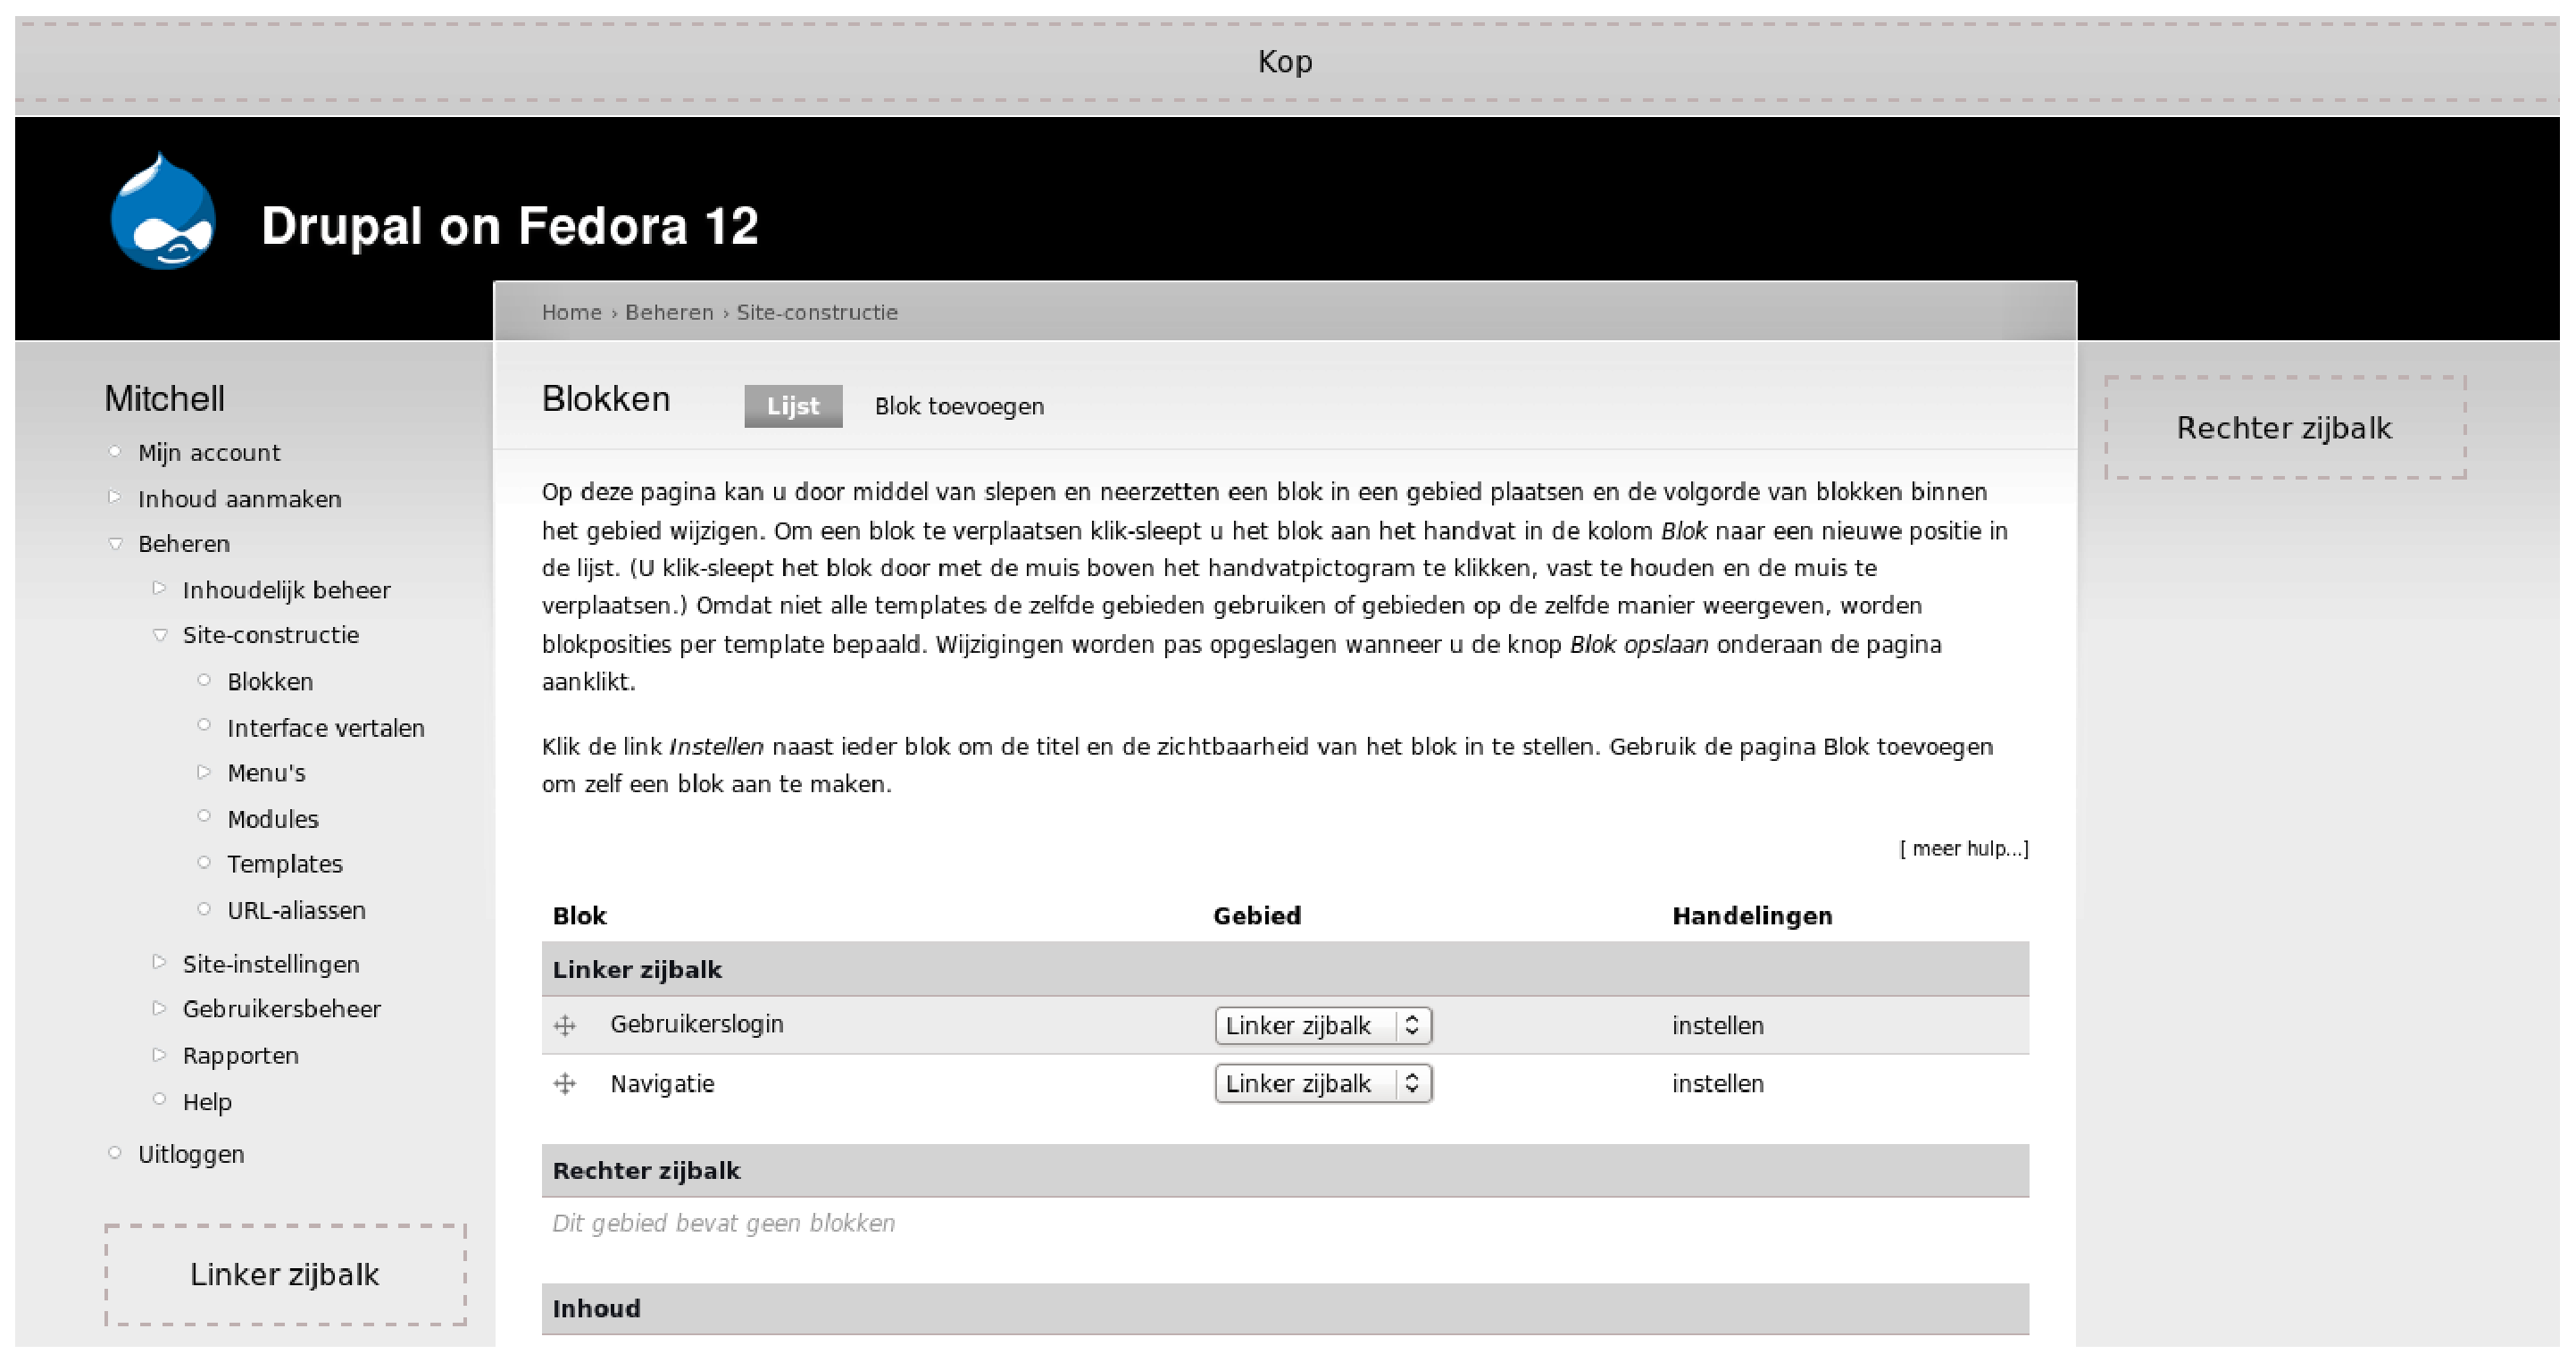
\includegraphics[scale=0.3,angle=0]{blokken-lijst}
   \caption{blokken-lijst.\label{white}}
 \end{figure}
 \subsection{Blok toevoegen} \index{blok toevoegen}
 Op deze pagina kunt u zelf een nieuw blok aanmaken. Nieuwe blokken zijn
 standaard uitgeschakeld en moeten op de pagina Blok beheren in een gebied geplaatst worden om te worden weergegeven.
 \begin{figure}[!h]
    \centering
   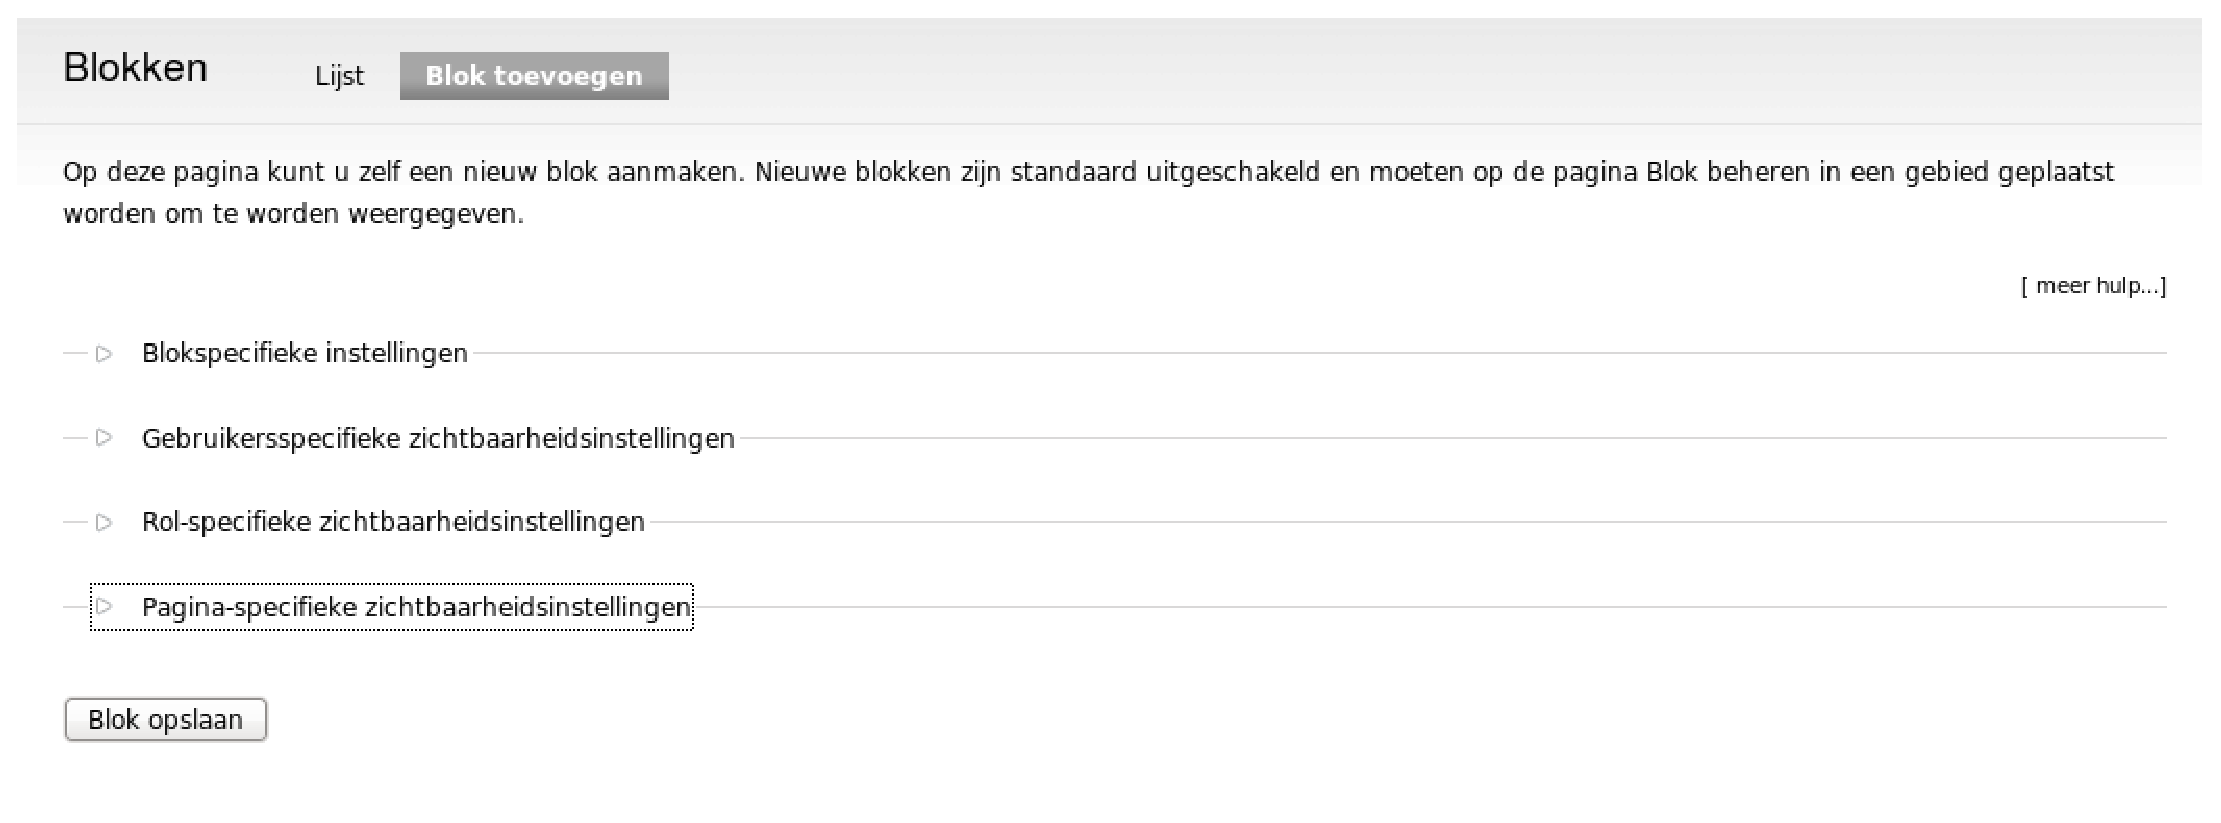
\includegraphics[scale=0.3,angle=0]{blok-toevoegen}
   \caption{blok-toevoegen.\label{white}}
 \end{figure}
\subsubsection{Blokspecifieke instellingen} \index{instellingen blok}
\begin{itemize}
\item Blokbeschrijving: Een korte beschrijving van het blok. Het wordt gebruikt op de blok overzichtspagina.
\item Bloktitel: De titel van een blok zoals getoond aan de gebruiker.
\item Blokinhoud: De inhoud van een blok zoals getoond aan de gebruiker.
\item Invoerformaat: Filtered HTML of Full HTML
\end{itemize}
 \begin{figure}[!h]
    \centering
   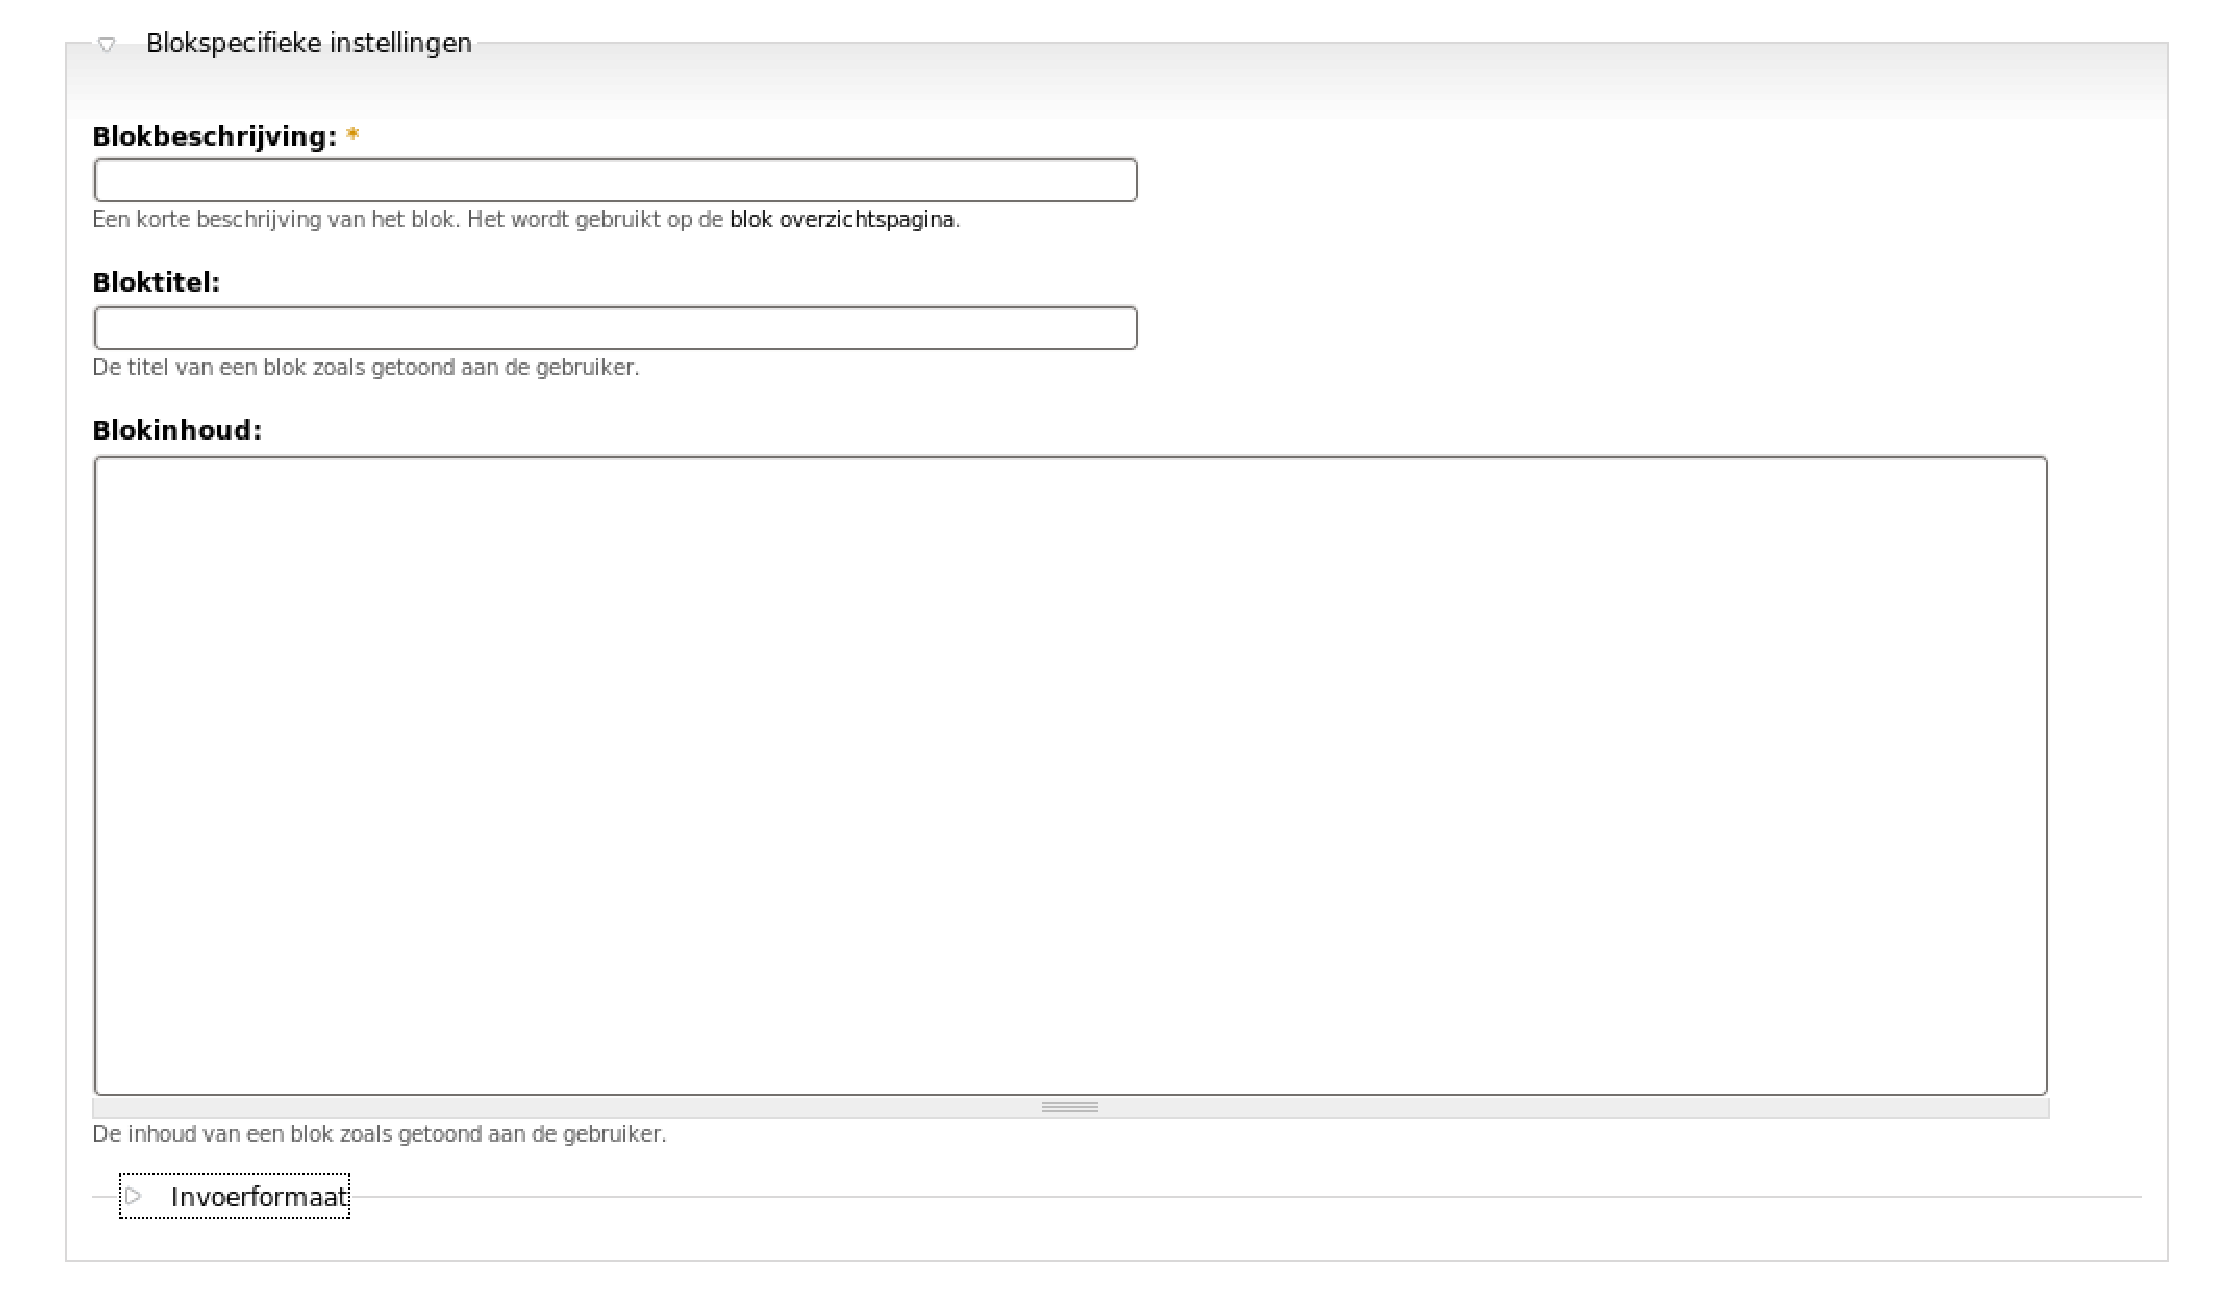
\includegraphics[scale=0.3,angle=0]{blok-specifieke-instellingen}
   \caption{blok-specifieke-instellingen.\label{white}}
 \end{figure}
\subsubsection{Gebruikersspecifieke zichtbaarheidsinstellingen}
\index{zichtbaarheidsinstellingen} Aangepaste zichtbaarheidsinstellingen: 
\begin{itemize}
\item Gebruikers kunnen niet kiezen of ze dit blok al dan niet willen zien.
\item Standaard dit blok weergeven. Individuele gebruikers kunnen ervoor kiezen het blok te verbergen.
\item Standaard dit blok verbergen. Individuele gebruikers kunnen ervoor kiezen het blok toch weer te geven.
\end{itemize}
Individuele gebruikers mogen de zichtbaarheid van dit blok in hun
gebruikersinstellingen aanpassen. 
\begin{figure}[!h]
    \centering
   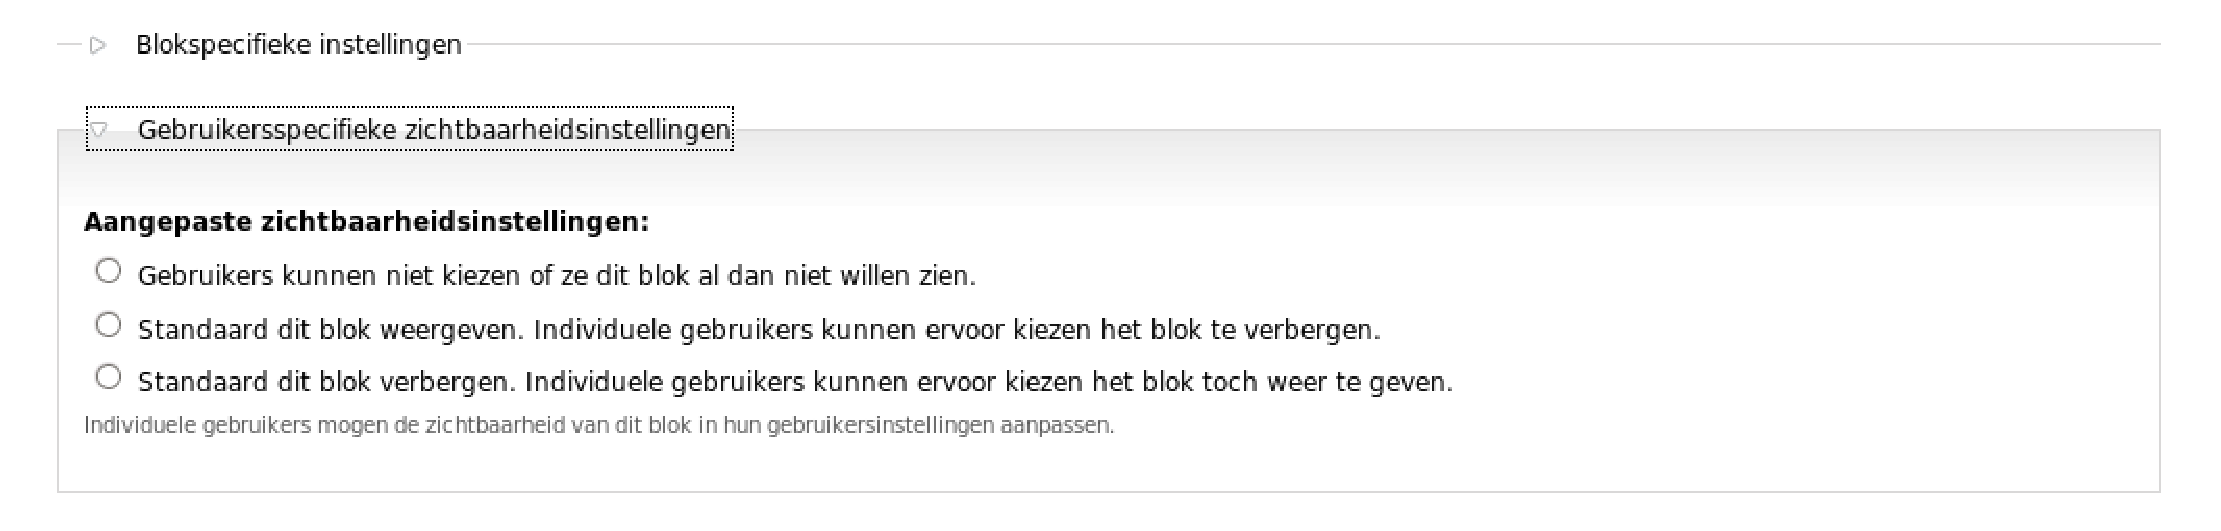
\includegraphics[scale=0.3,angle=0]{blok-gebruikers-specifieke}
   \caption{blok-gebruikers-specifieke.\label{white}}
 \end{figure} 
\subsubsection{Rol-specifieke zichtbaarheidsinstellingen}
Blok voor bepaalde rollen weergeven:  
\begin{itemize}
\item admin
\item anonymous user
\item authenticated user
\end{itemize}
Dit blok is alleen zichtbaar voor bepaalde rollen. Als u geen rollen selecteert is het blok voor alle gebruikers zichtbaar.
\begin{figure}[!h]
    \centering
   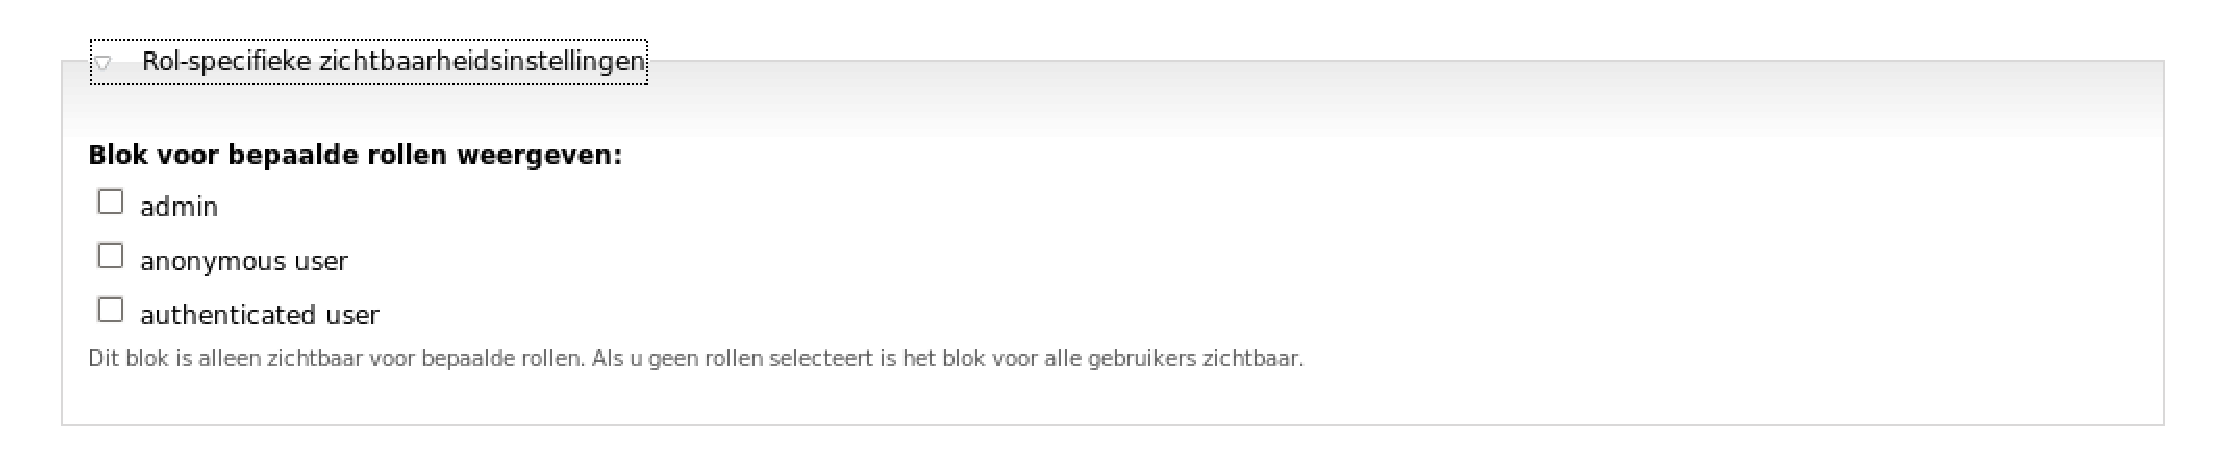
\includegraphics[scale=0.3,angle=0]{blok-rol-specifieke}
   \caption{blok-rol-specifieke.\label{white}}
 \end{figure} 
\subsubsection{Pagina-specifieke zichtbaarheidsinstellingen}
Blok op bepaalde pagina's weergeven:   
\begin{itemize}
\item Weergeven op elke pagina behalve op de vermelde pagina's.
\item Alleen weergeven op de vermelde pagina's.
\item Alleen weergeven wanneer de volgende PHP-code resulteert in TRUE. (PHP-mode, alleen voor experts).
\end{itemize}
Geef \'e\'en pagina per regel op, als Drupal-paden. Het '*'-teken is een
jokerteken. Voorbeeldpaden zijn 'blog' voor de blog-pagina en 'blog/*' voor elke
persoonlijke blog. '$<$front$>$' is de voorpagina. Als de PHP-modus wordt
gekozen geef dan de PHP-code op tussen $<$?php ?$>$. Merk op dat het uitvoeren
van incorrecte PHP-code uw Drupalsite defect kan maken. 
\begin{figure}[!h]
    \centering
   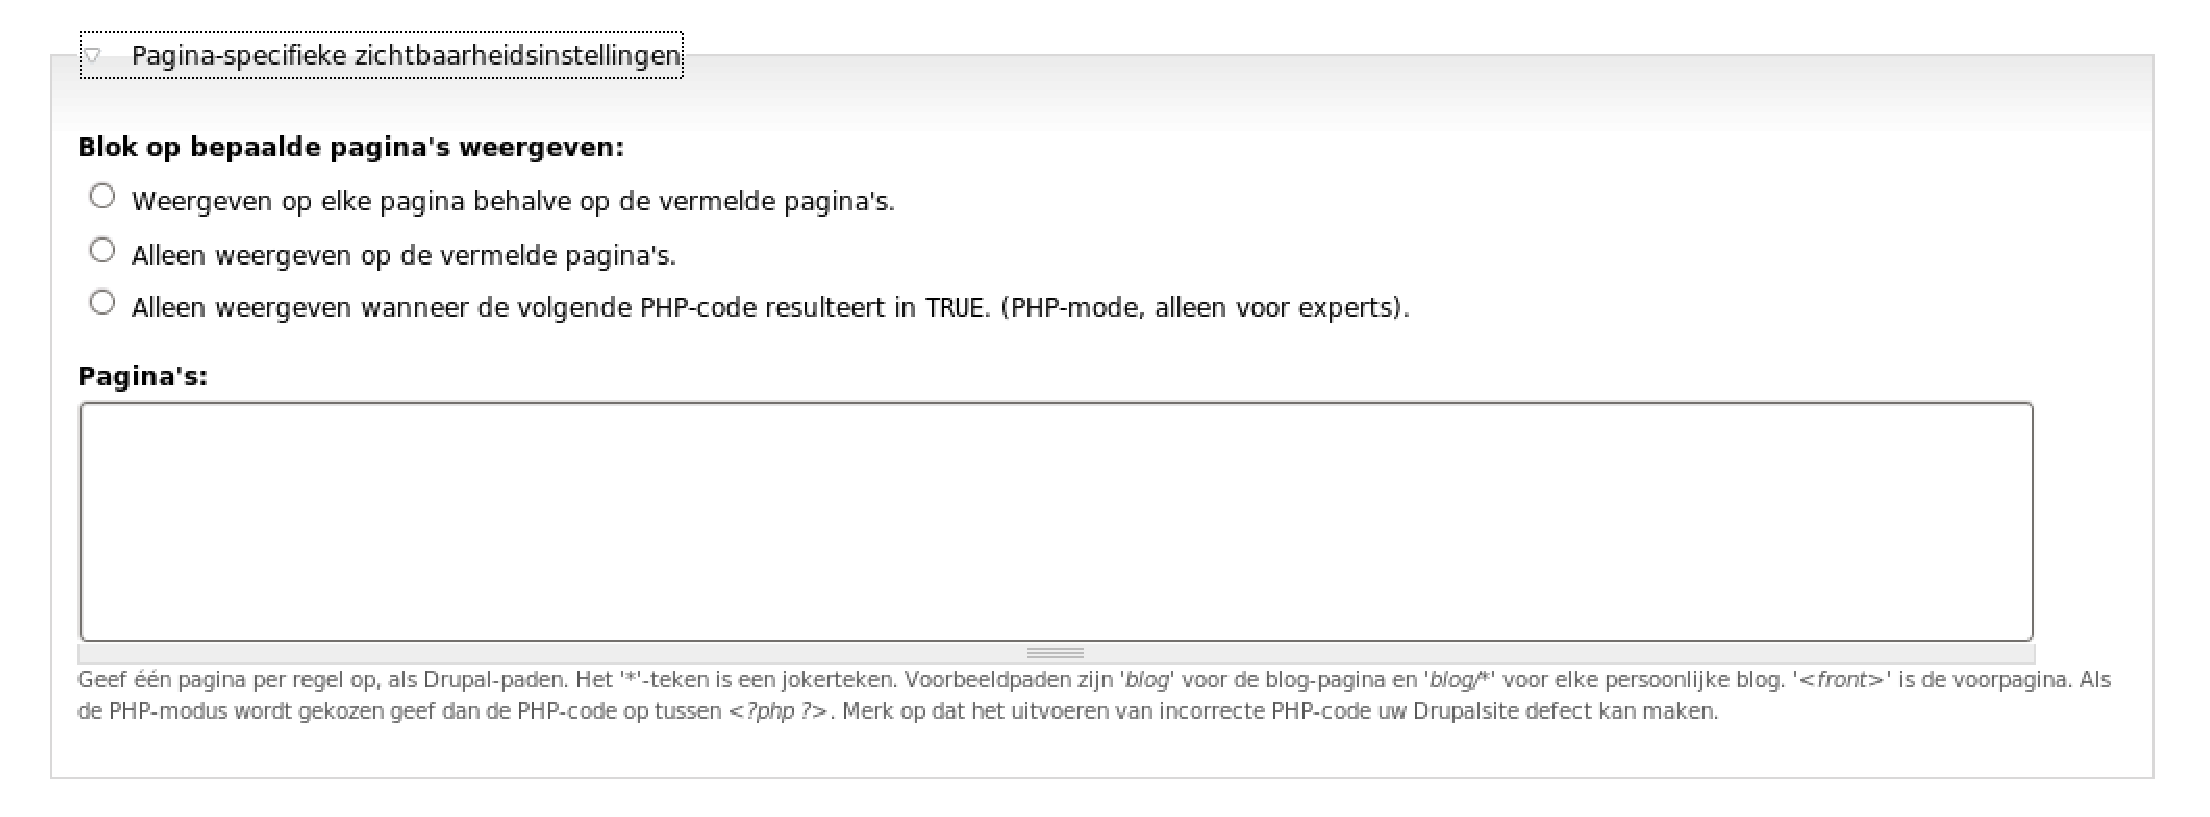
\includegraphics[scale=0.3,angle=0]{blok-pagina-specifieke}
   \caption{blok-pagina-specifieke.\label{white}}
 \end{figure} 



\section{Interface vertalen} \index{vertalen}
Deze pagina geeft een overzicht van vertaalbare tekenreeksen. Vertaalbare tekenreeksen 
worden weergegeven in zogenaamde 'tekstgroepen'. Modules kunnen extra tekstgroepen toevoegen 
die andere vertaalbare tekenreeksen bevatten. Omdat tekstgroepen een mogelijkheid bieden 
om tekenreeksen te groeperen, kunnen de tekstgroepen gebruikt worden om de vertaalinspanning 
te richten op bepaalde gebieden van de Drupal-interface.
\begin{figure}[!h]
    \centering
   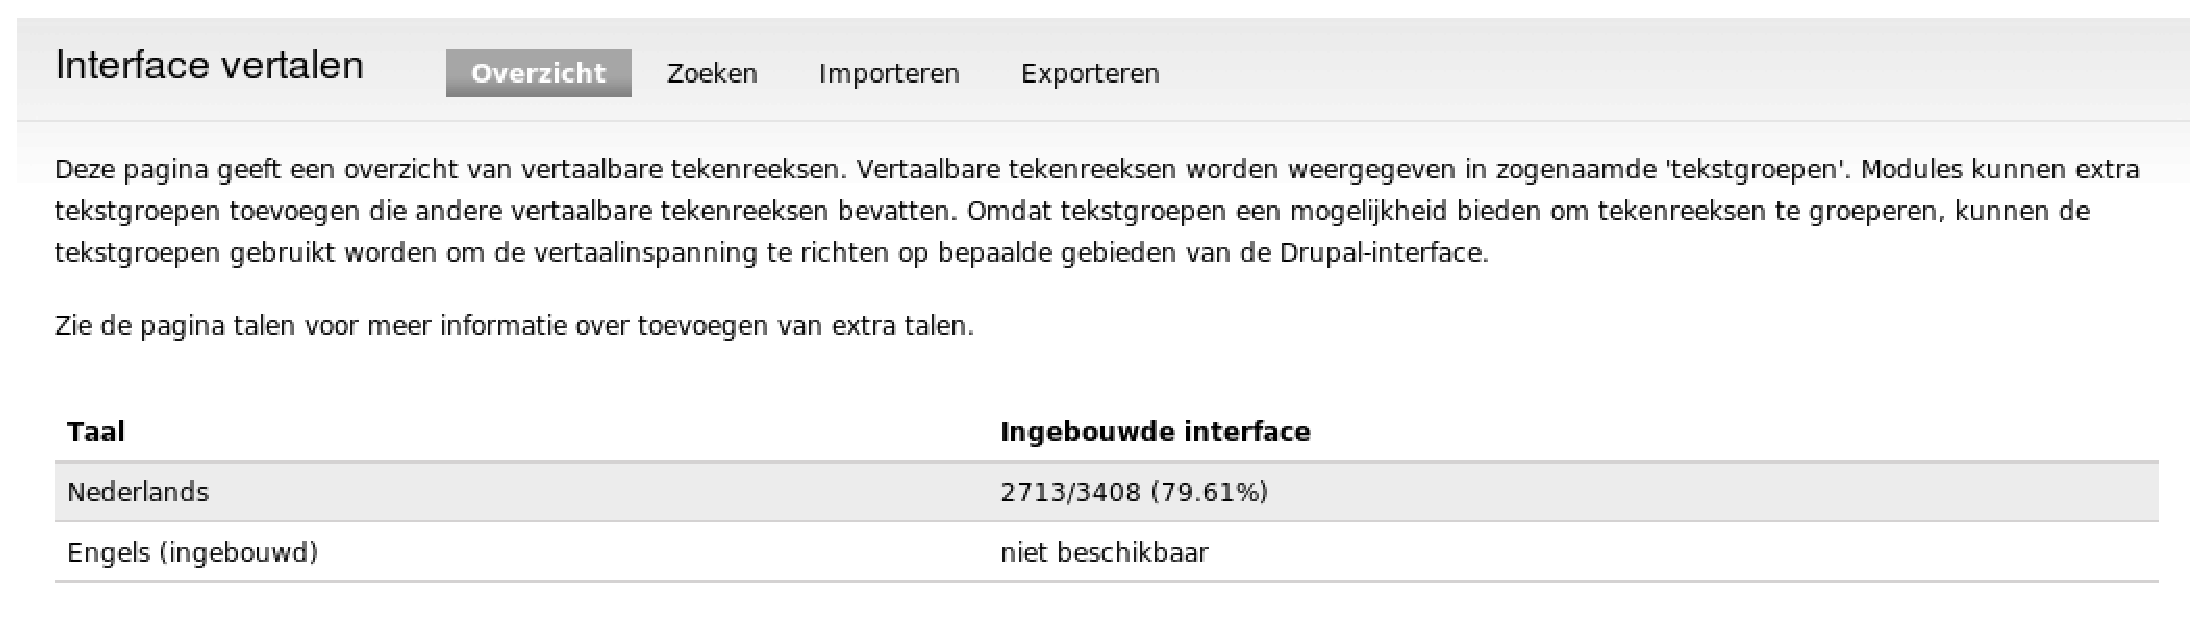
\includegraphics[scale=0.3,angle=0]{interfacevertalen-overzicht}
   \caption{interfacevertalen-overzicht.\label{white}}
 \end{figure}

\subsection{Interface vertalen - zoeken}
Op deze pagina kan een vertaler zoeken naar specifieke vertaalde en onvertaalde
tekenreeksen en vertalingen maken of bestaande vertalingen bijwerken. Merk op: 
voor het vertalen van vele tekenreeksen is het handiger om de tekenreeksen te 
exporteren en offline met een Gettext-editor te vertalen. 
Zoeken naar tekenreeksen kan beperkt worden tot een specifieke tekstgroep of een specifieke taal.
\begin{figure}[!h]
    \centering
   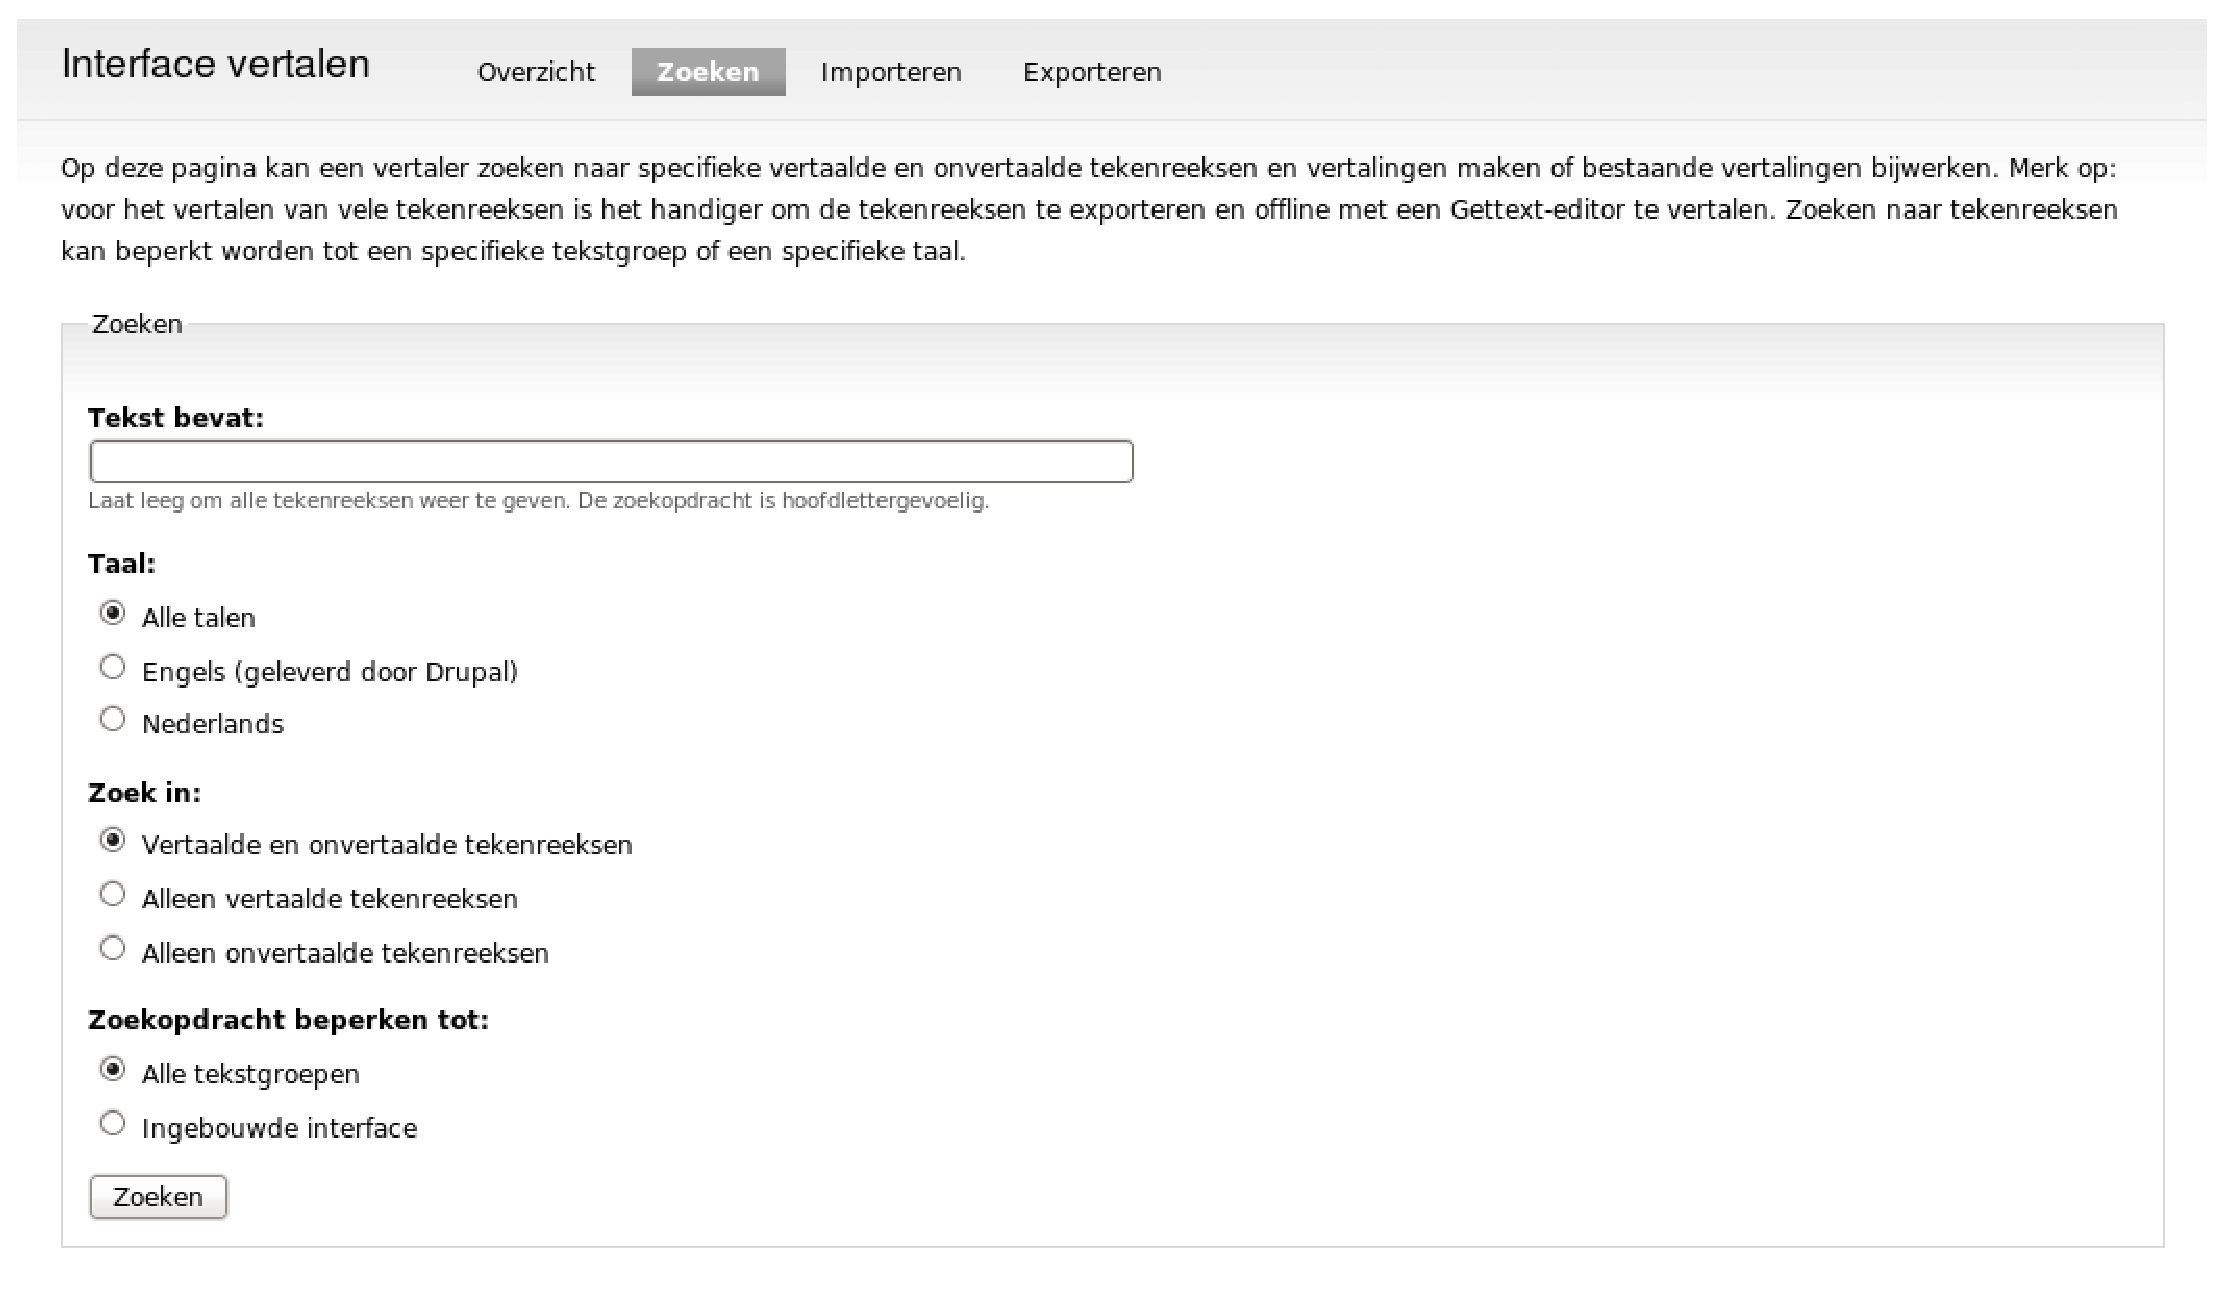
\includegraphics[scale=0.3,angle=0]{interfacevertalen-zoeken}
   \caption{interfacevertalen-zoeken.\label{white}}
 \end{figure}
 
\subsection{Importeren} \index{importeren}
Op deze pagina kunt u een vertaling als Gettext Portable Object (.po)-bestand importeren. 
Deze bestanden zijn gewoonlijk onderdeel van een vertaalpakket. Als een .po-bestand 
offline met een Gettext-editor wordt gewijzigd, kan u het bijgewerkte bestand op deze pagina 
importeren. Importeren van een .po-bestand kan enige tijd duren.
\\
Weet dat de .po-bestanden (indien aanwezig) automatisch ge\"importeerd worden
als een nieuwe module of template ingeschakeld wordt of als nieuwe talen worden toegevoegd. 
Omdat met deze pagina slechts \'e\'en .po-bestand tegelijkertijd ge\"importeerd
kan worden, kan het eenvoudiger zijn om een vertaalpakket te downloaden en in de Drupal-installatiemap 
uit te pakken en daarna de taal toe te voegen. Alle .po-bestanden in het vertaalpakket 
worden dan automatisch ge\"importeerd. Vertaalpakketten kunnen worden op de
Drupal Translations-pagina gedownload worden. \begin{figure}[!h]
    \centering
   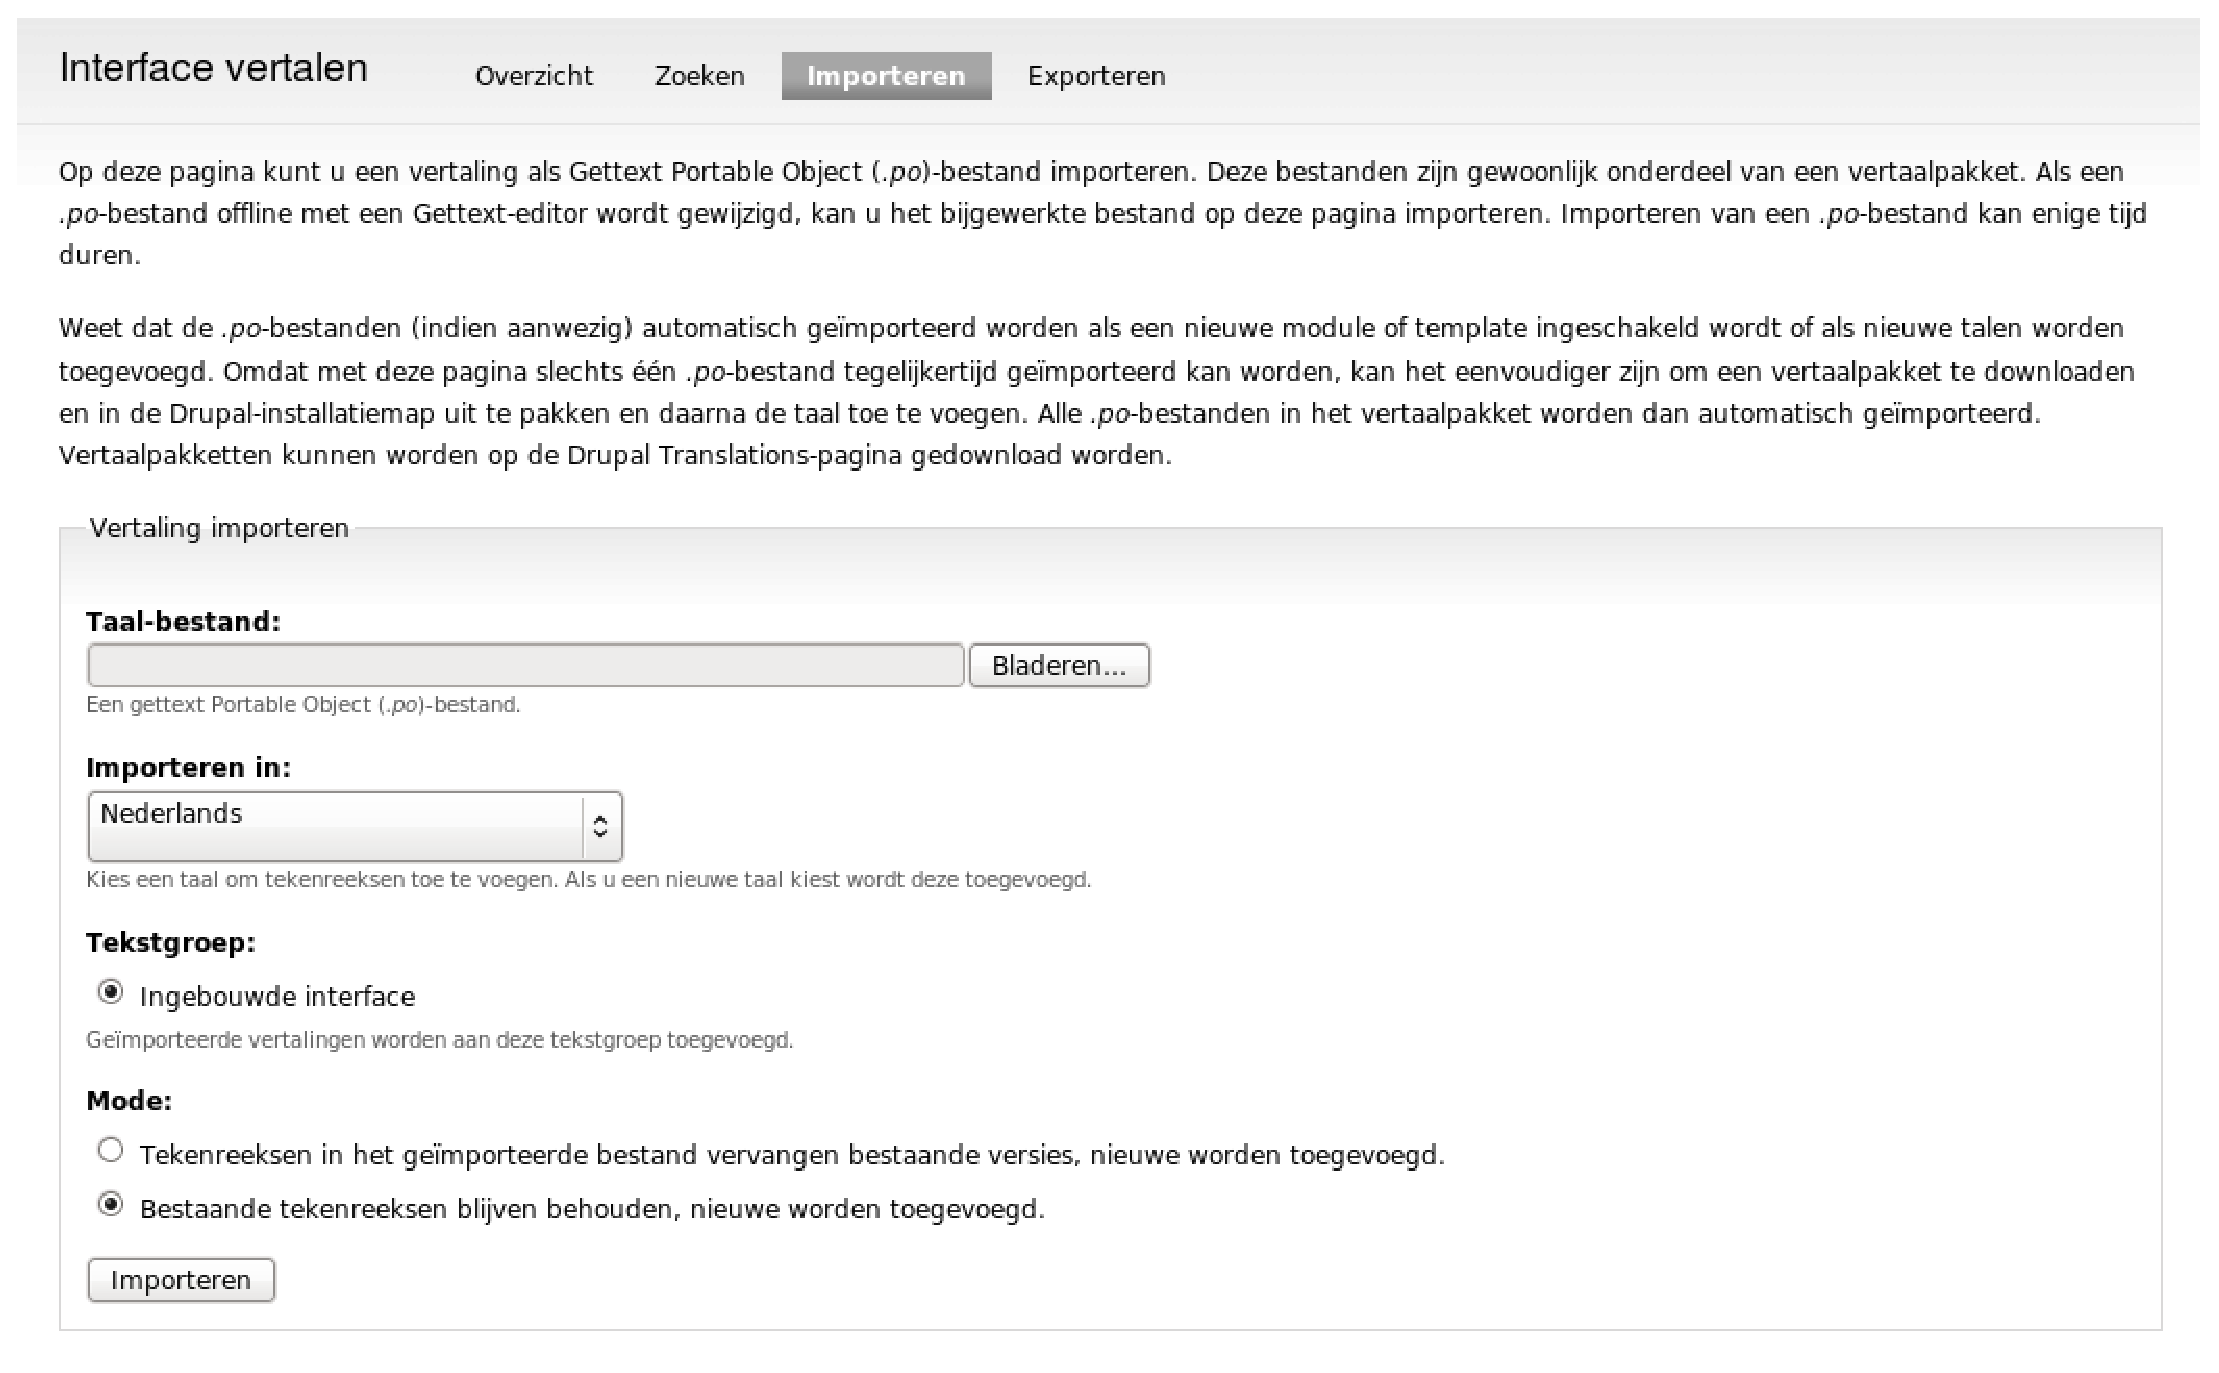
\includegraphics[scale=0.3,angle=0]{interfacevertalen-importeren}
   \caption{interfacevertalen-importeren.\label{white}}
 \end{figure}
 
\subsection{Exporteren} \index{exporteren} 
Op deze pagina kunt u vertaalde Drupal-tekenreeksen exporteren. De tekenreeksen kunnen in twee 
formaten als bestand ge\"exporteerd worden. Het Gettext Portable Object
(.po)-formaat, met daarin zowel de bron als de vertaalde tekenreeksen, of het Gettext Portable Object Template (.pot)-formaat, 
met daarin alleen de bron-tekenreeksen. Het .po-formaat wordt gebruikt om vertaling met anderen te delen, 
het .pot-formaat om met een Gettext-editor een nieuwe vertaling te maken.
\begin{figure}[!h]
    \centering
   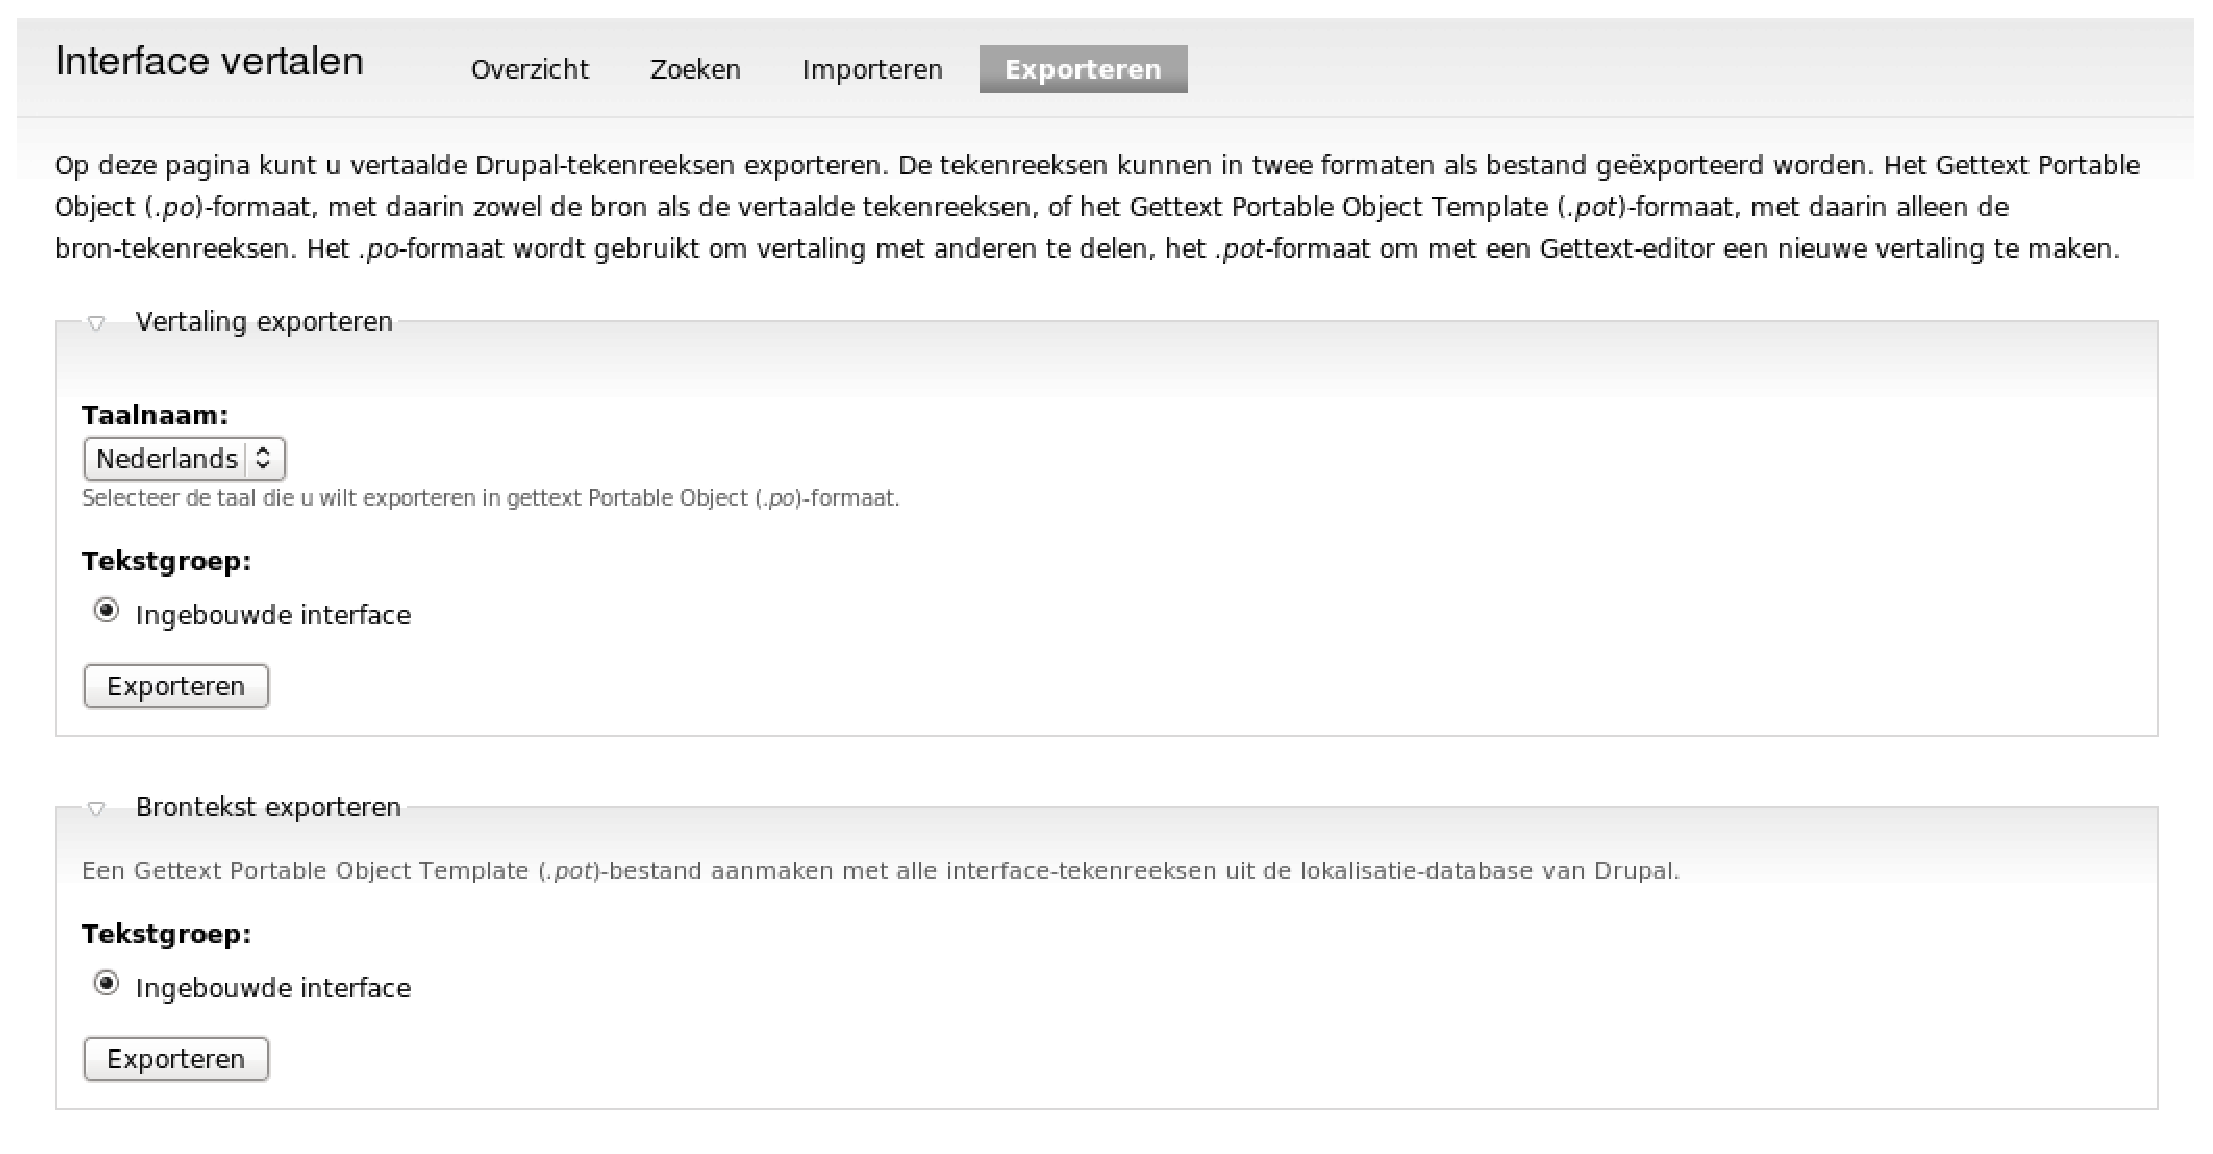
\includegraphics[scale=0.3,angle=0]{interfacevertalen-exporteren}
   \caption{interfacevertalen-exporteren.\label{white}}
 \end{figure}

\section{Menu's} \index{menu}
Navigatiemenu, \index{navigatiemenu} primaire \index{primaire links} en
secundaire links \index{secundaire links} beheren, menu-onderdelen hernoemen en
menu's reorganiseren.

\subsection{Menu-module} \index{menu-module}
De Menu-module biedt de mogelijkheid om het Drupal menu-systeem te beheren en in te stellen. 
Menu's zijn een verzameling van links (menu-onderdelen) die worden gebruikt om binnen de 
website te navigeren en worden met behulp van Drupal-blokken binnen een pagina gepositioneerd 
en weergegeven. Standaard worden tijdens installatie drie menu's aangemaakt: Navigatie, Primaire links en Secundaire links. 
Het Navigatiemenu bevat de menu-onderdelen die nodig zijn om de website te beheren en wordt vaak in de linker of rechter 
zijbalk weergegeven. De meeste Drupal-templates ondersteunen Primaire links en Secundaire links en geven deze menu's in 
kop of voet van de pagina weer. Standaard bevatten Primaire links en Secundaire links geen menu-onderdelen, maar deze 
kunnen door de beheerder met website-specifieke menu-onderdelen worden gevuld.
\\
De pagina menu's bevat alle menu's die op de site beschikbaar zijn. Selecteer een menu om menu-onderdelen toe 
te voegen, te wijzingen of de volgorde van menu-onderdelen binnen het menu te veranderen. Op de pagina menu 
toevoegen kunt u een menu toevoegen (Op de pagina Blokken beheren kunt u het blok dat dit menu bevat inschakelen).

\subsection{Menu's weergeven}
Menu's zijn een verzameling van links (menu-onderdelen) die worden gebruikt om
binnen de website te navigeren. Hier onder vindt u alle menu's die op de site beschikbaar zijn. 
Selecteer een menu uit de lijst om de bijbehorende menu-onderdelen te beheren.
\begin{figure}[!h]
    \centering
   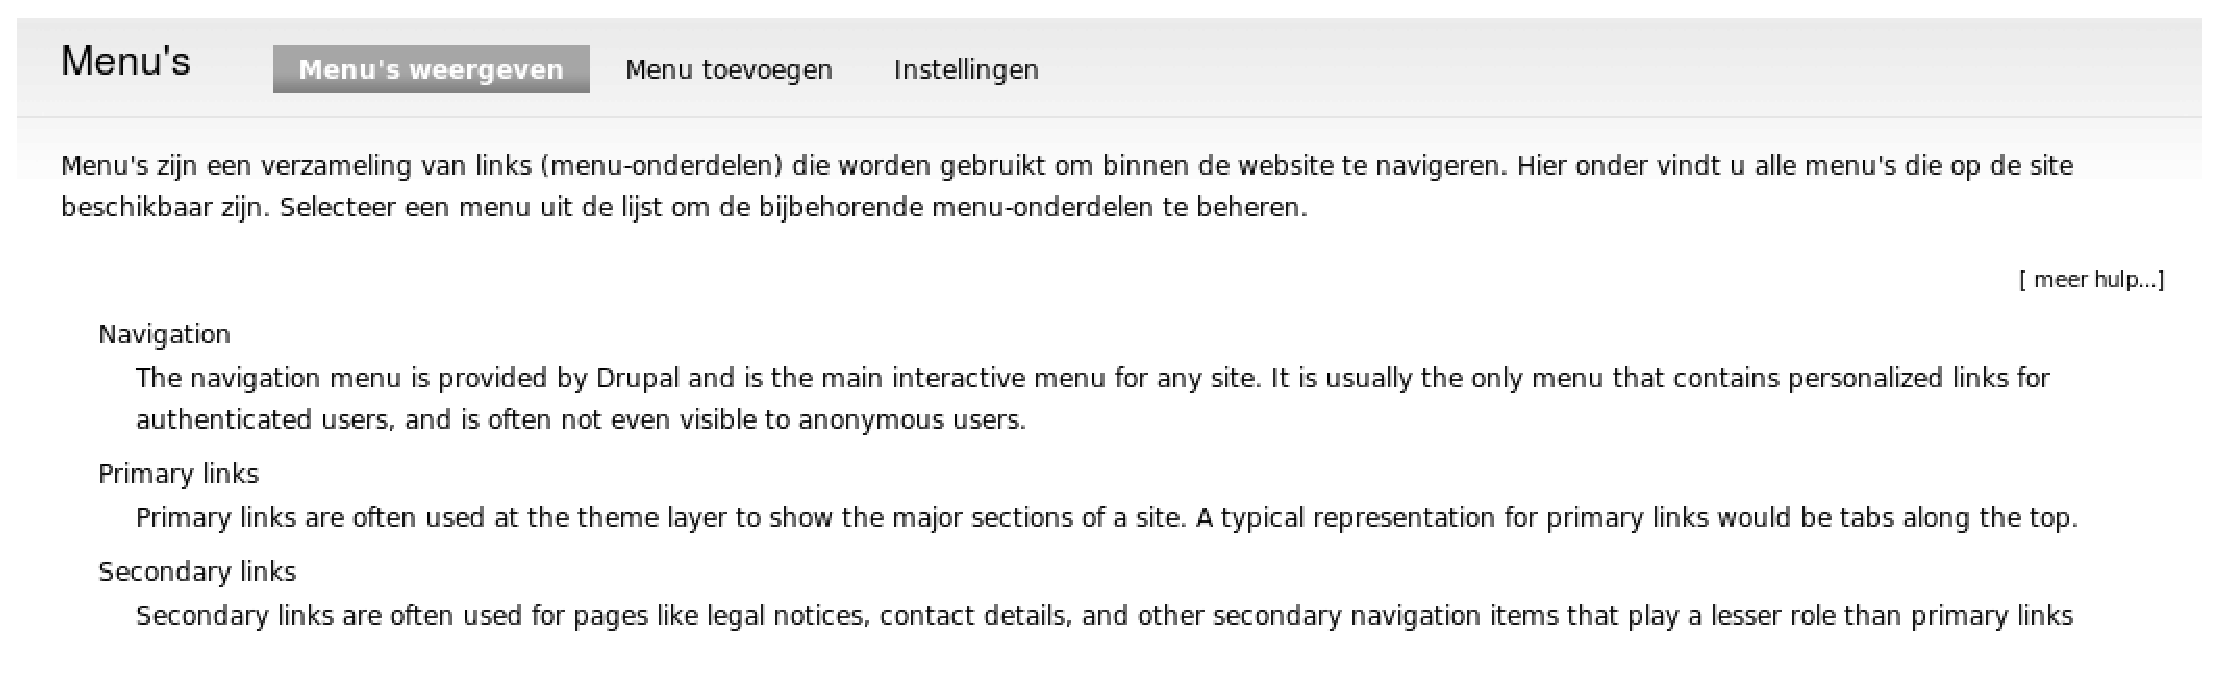
\includegraphics[scale=0.3,angle=0]{menu-weergeven}
   \caption{menu-weergeven.\label{white}}
 \end{figure}

\subsection{Menu toevoegen}
Geef de naam op voor een nieuw menu. Vergeet niet het nieuw aangemaakte blok in
de pagina blokbeheer in te schakelen.
\begin{figure}[!h]
    \centering
   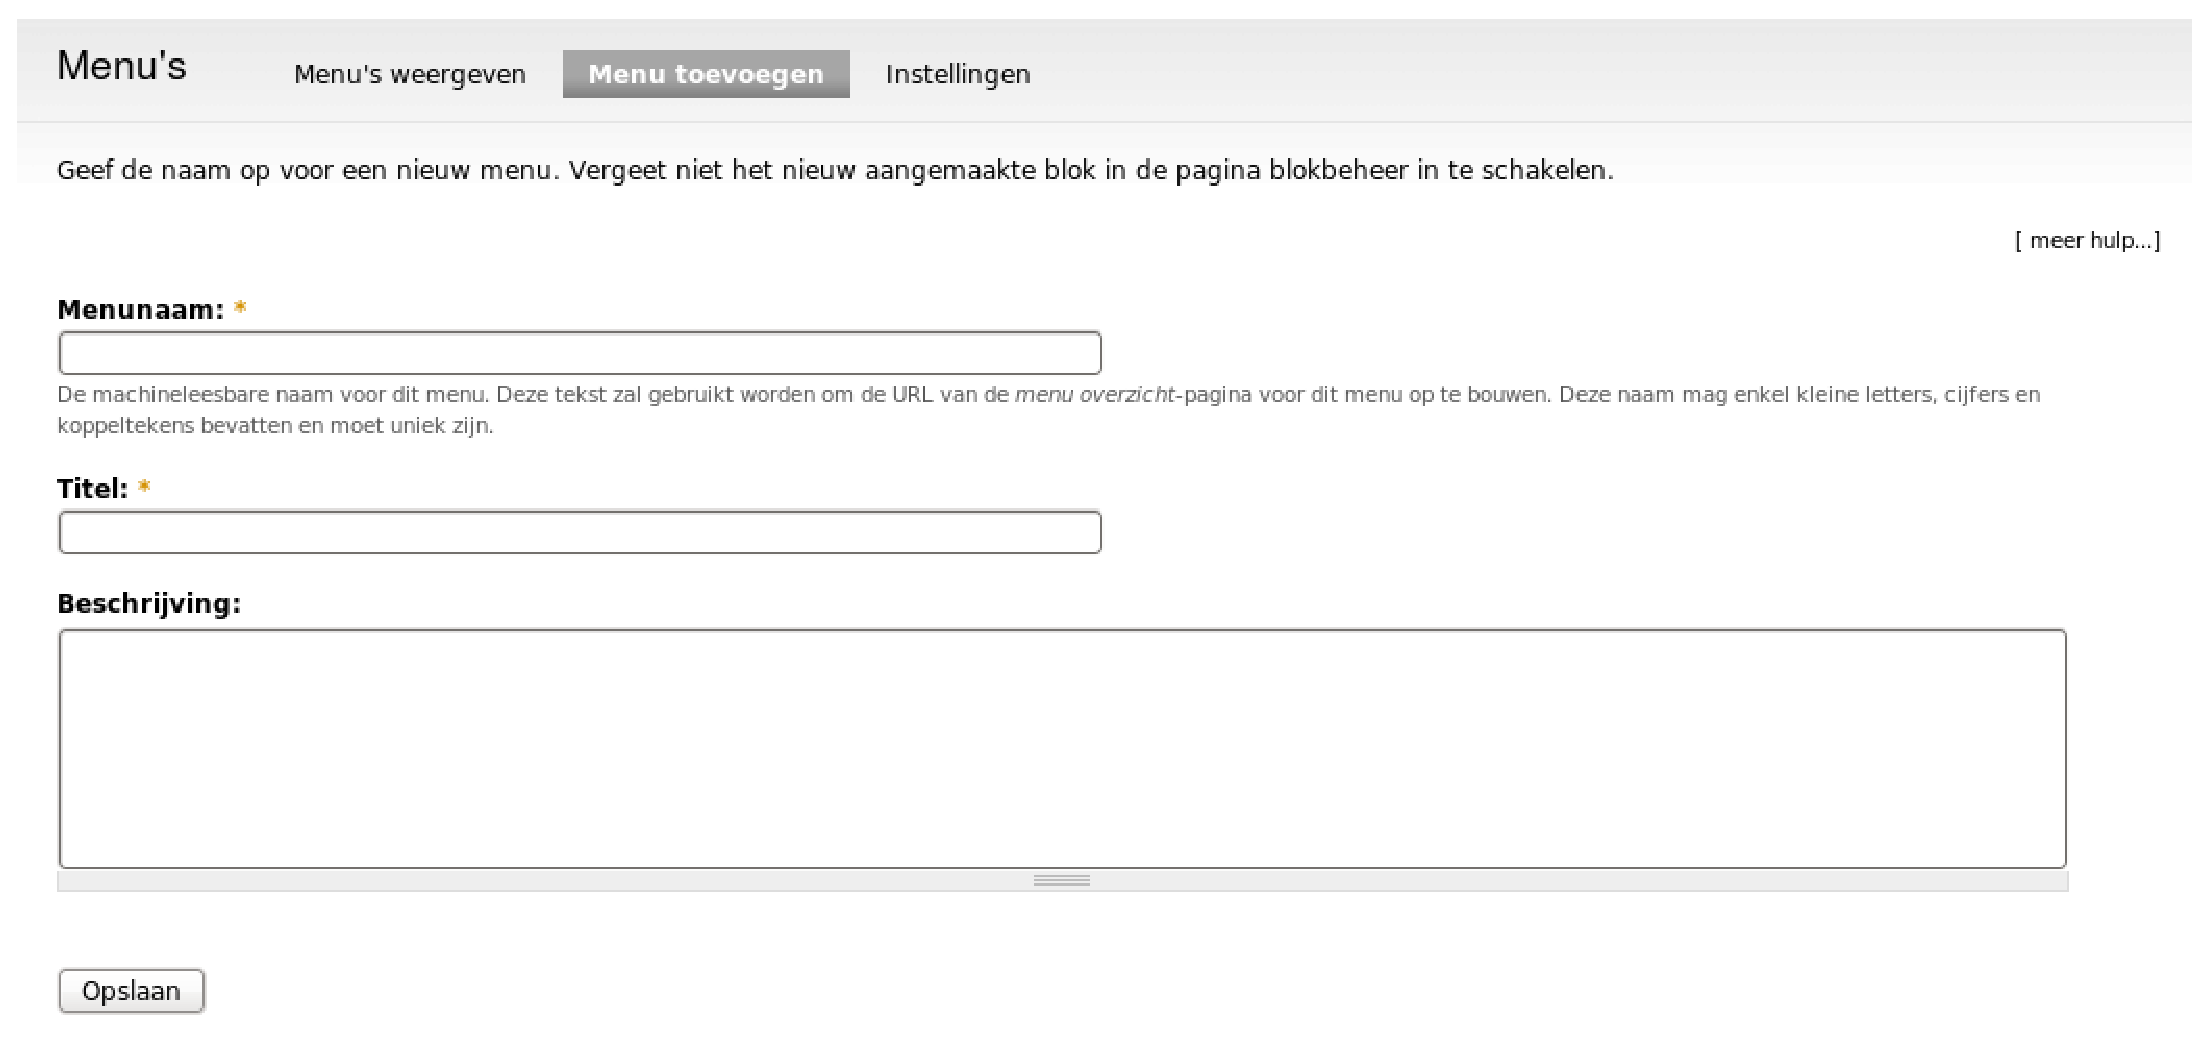
\includegraphics[scale=0.3,angle=0]{menu-toevoegen}
   \caption{menu-toevoegen.\label{white}}
 \end{figure}

\subsection{Instellingen}
De Menu-module maakt het mogelijk om in het node-invoer- en bewerkingsformulier
een menu-link naar de node aan te maken. De volgende optie bepaalt het standaardmenu waaraan een nieuwe link zal worden toegevoegd. 
\begin{figure}[!h]
    \centering
   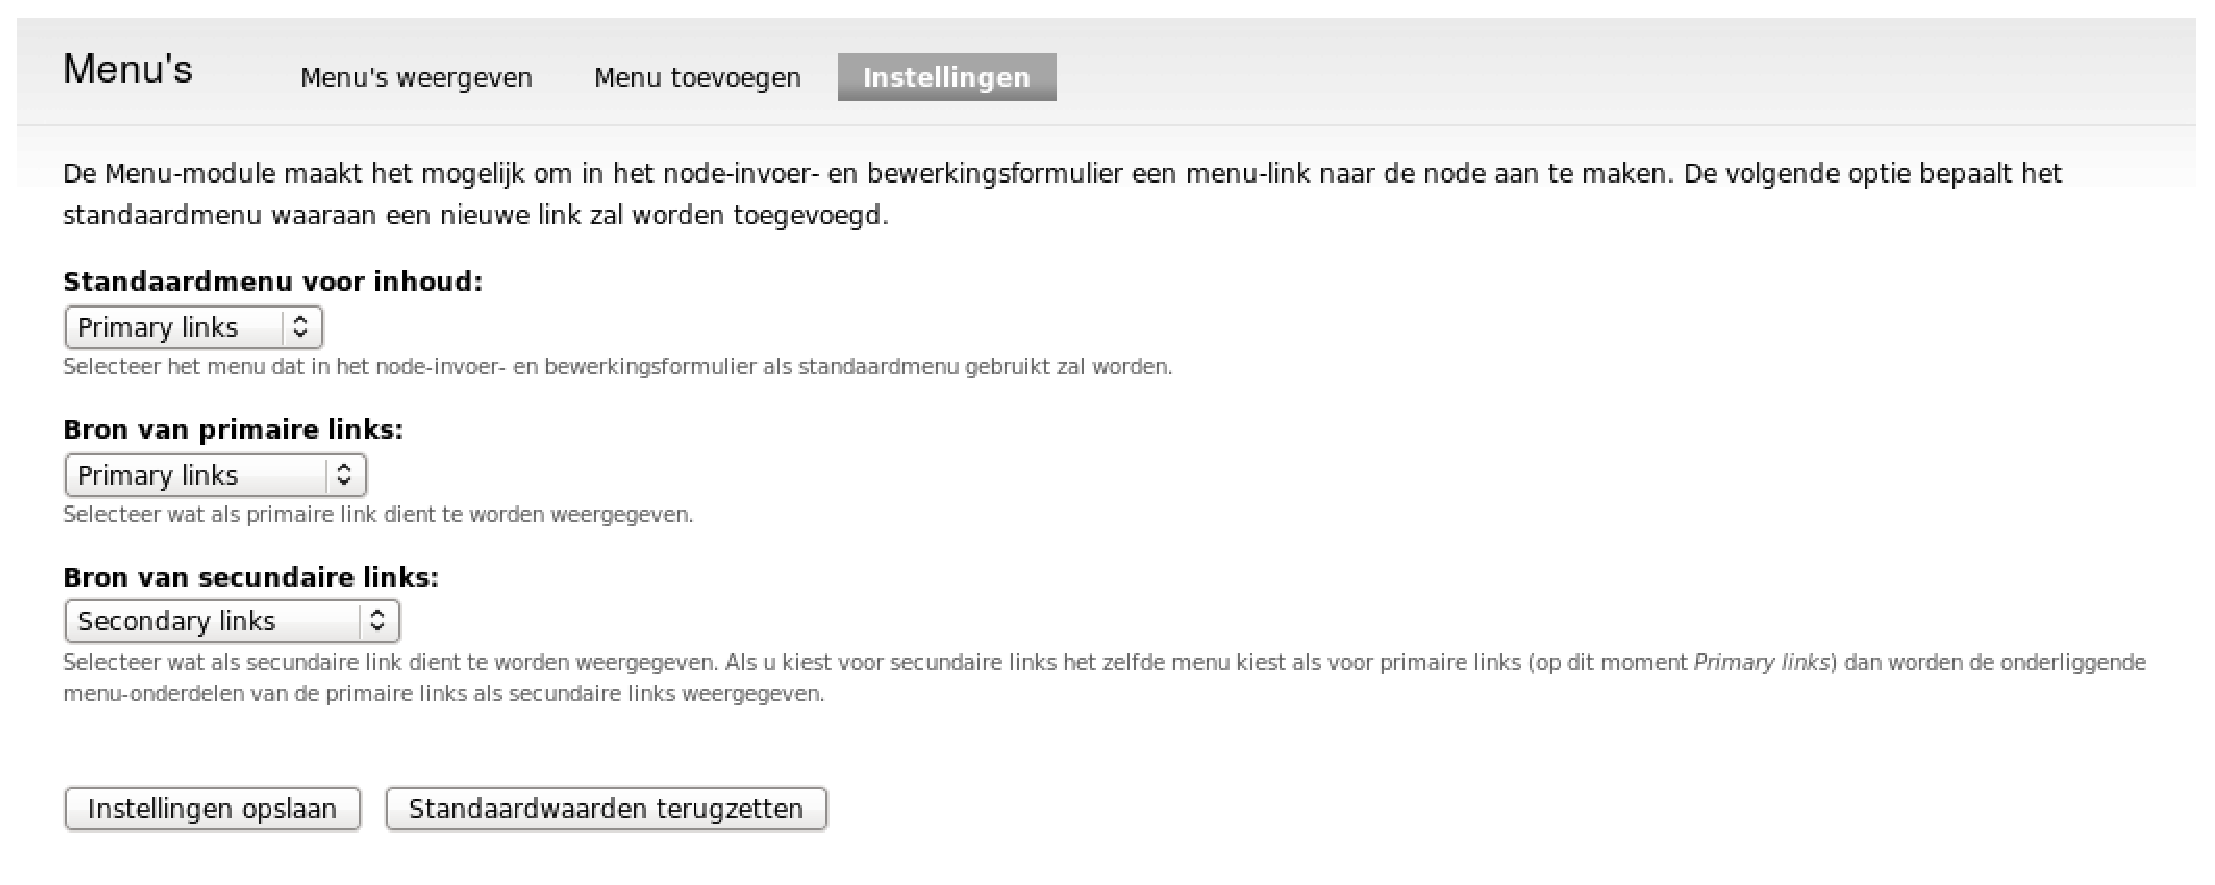
\includegraphics[scale=0.3,angle=0]{menu-instellingen-01}
   \caption{menu-instellingen-01.\label{white}}
 \end{figure}

\subsection{Navigation}
Om menu-onderdelen te verplaatsen klik-sleept u deze aan het handvat in de kolom
Menu-item naar een nieuwe positie in de lijst. (U klik-sleept het blok door met de muis boven het handvatpictogram te klikken, 
vast te houden en de muis te verplaatsen.) Wijzigingen worden pas opgeslagen wanneer u de knop Opslaan onderaan de pagina aanklikt.
\begin{figure}[!h]
    \centering
   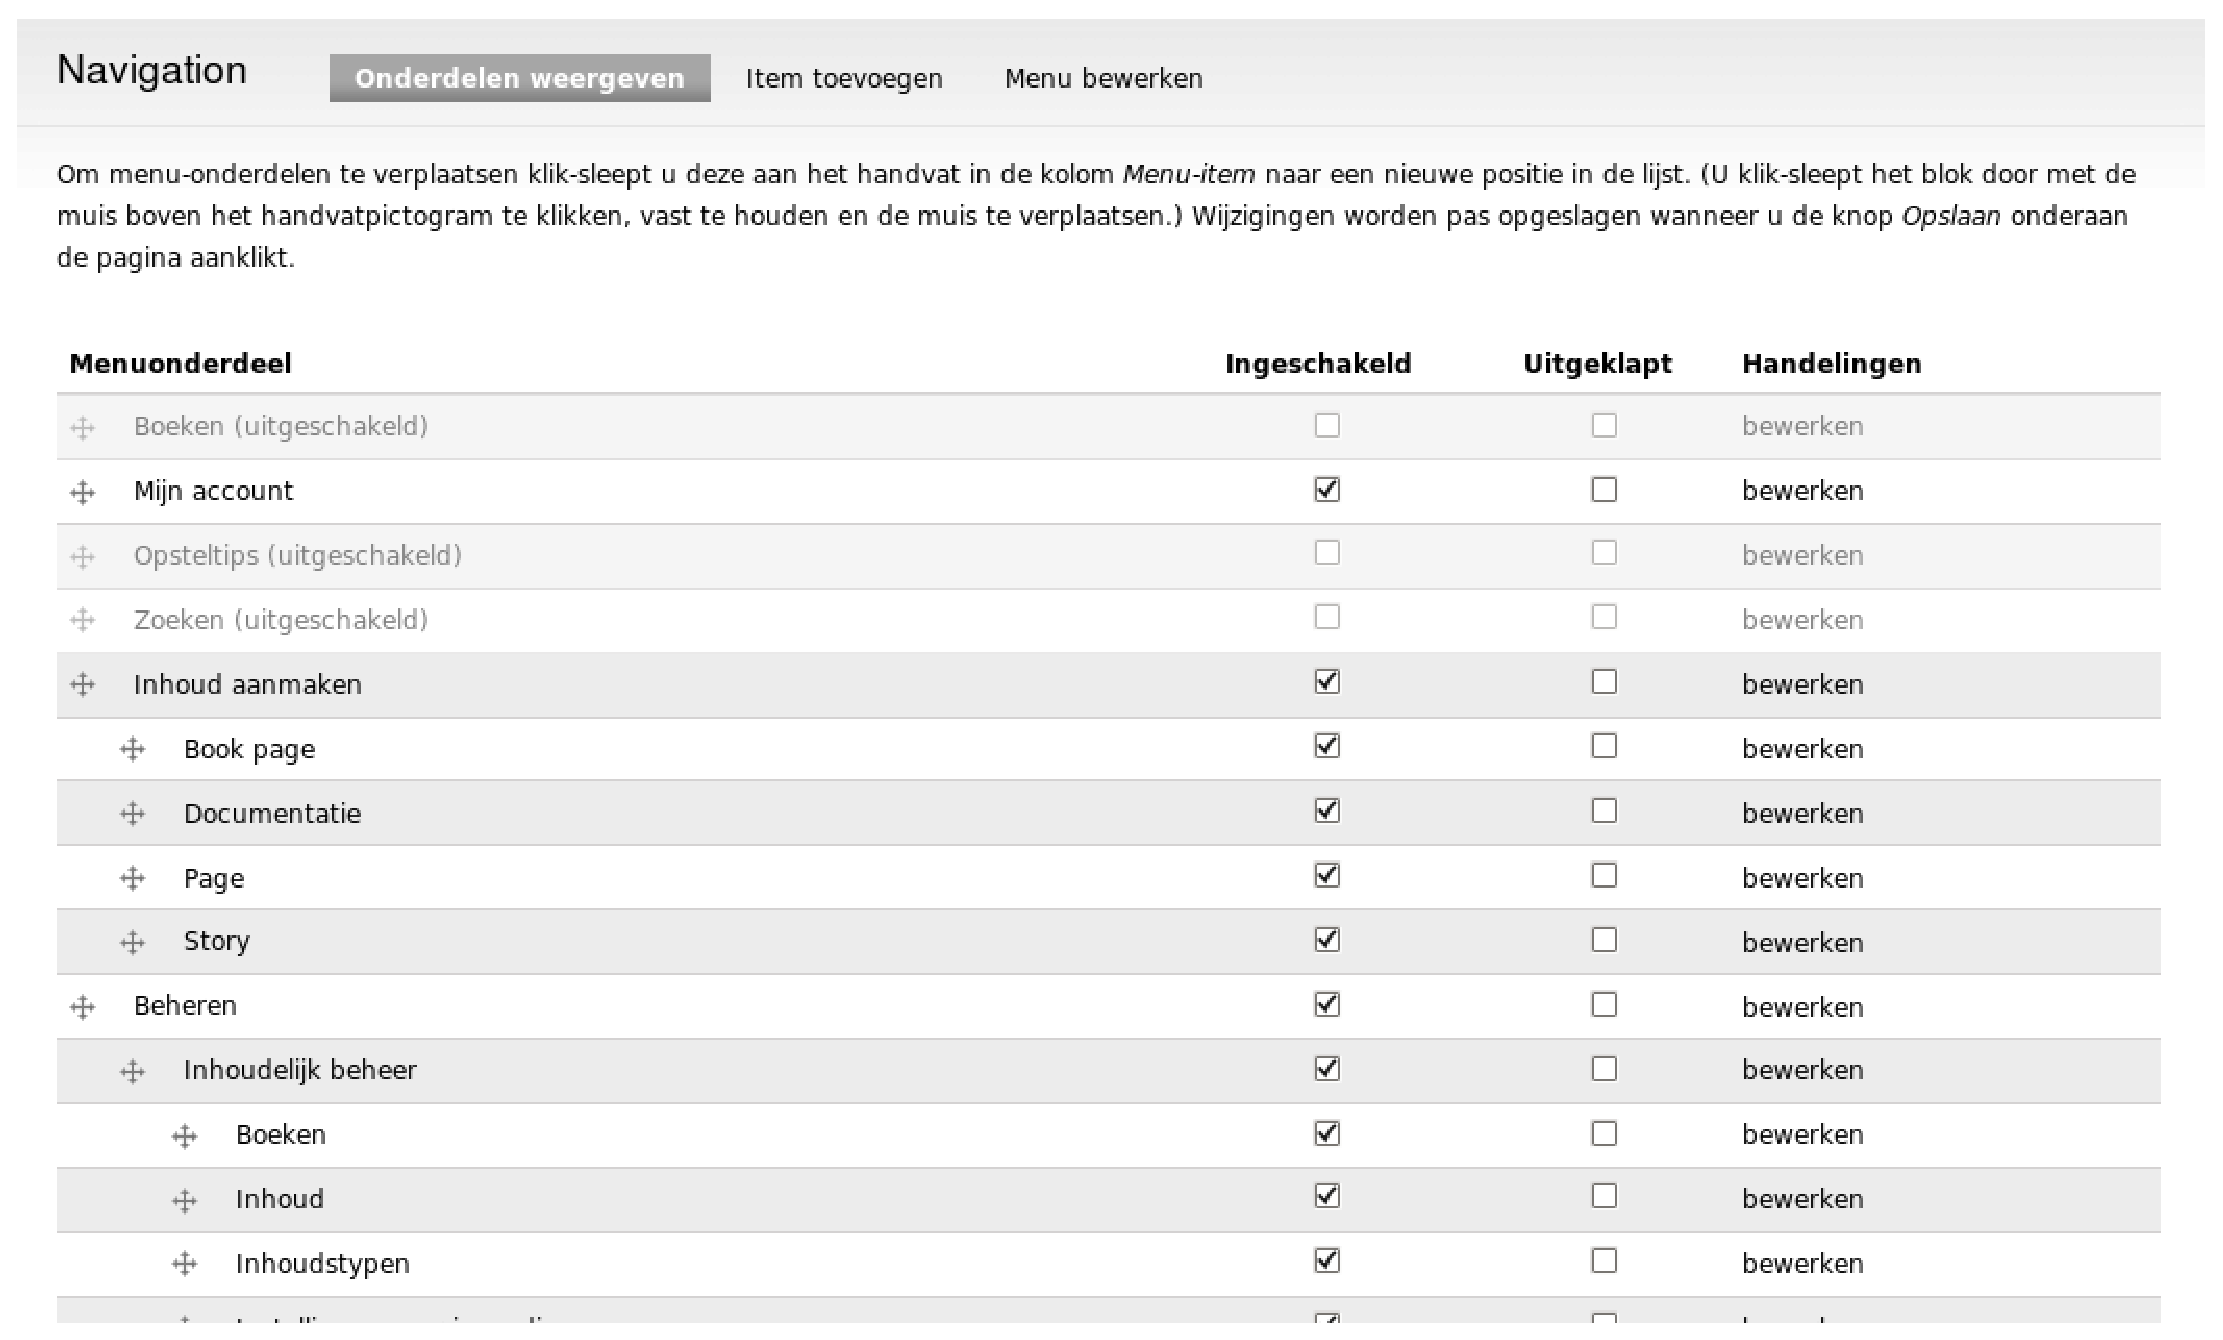
\includegraphics[scale=0.3,angle=0]{nav-onderdelen-weergeven}
   \caption{nav-onderdelen-weergeven.\label{white}}
 \end{figure}
% \subsubsection{item toevoegen}
% \begin{figure}[!h]
%     \centering
%    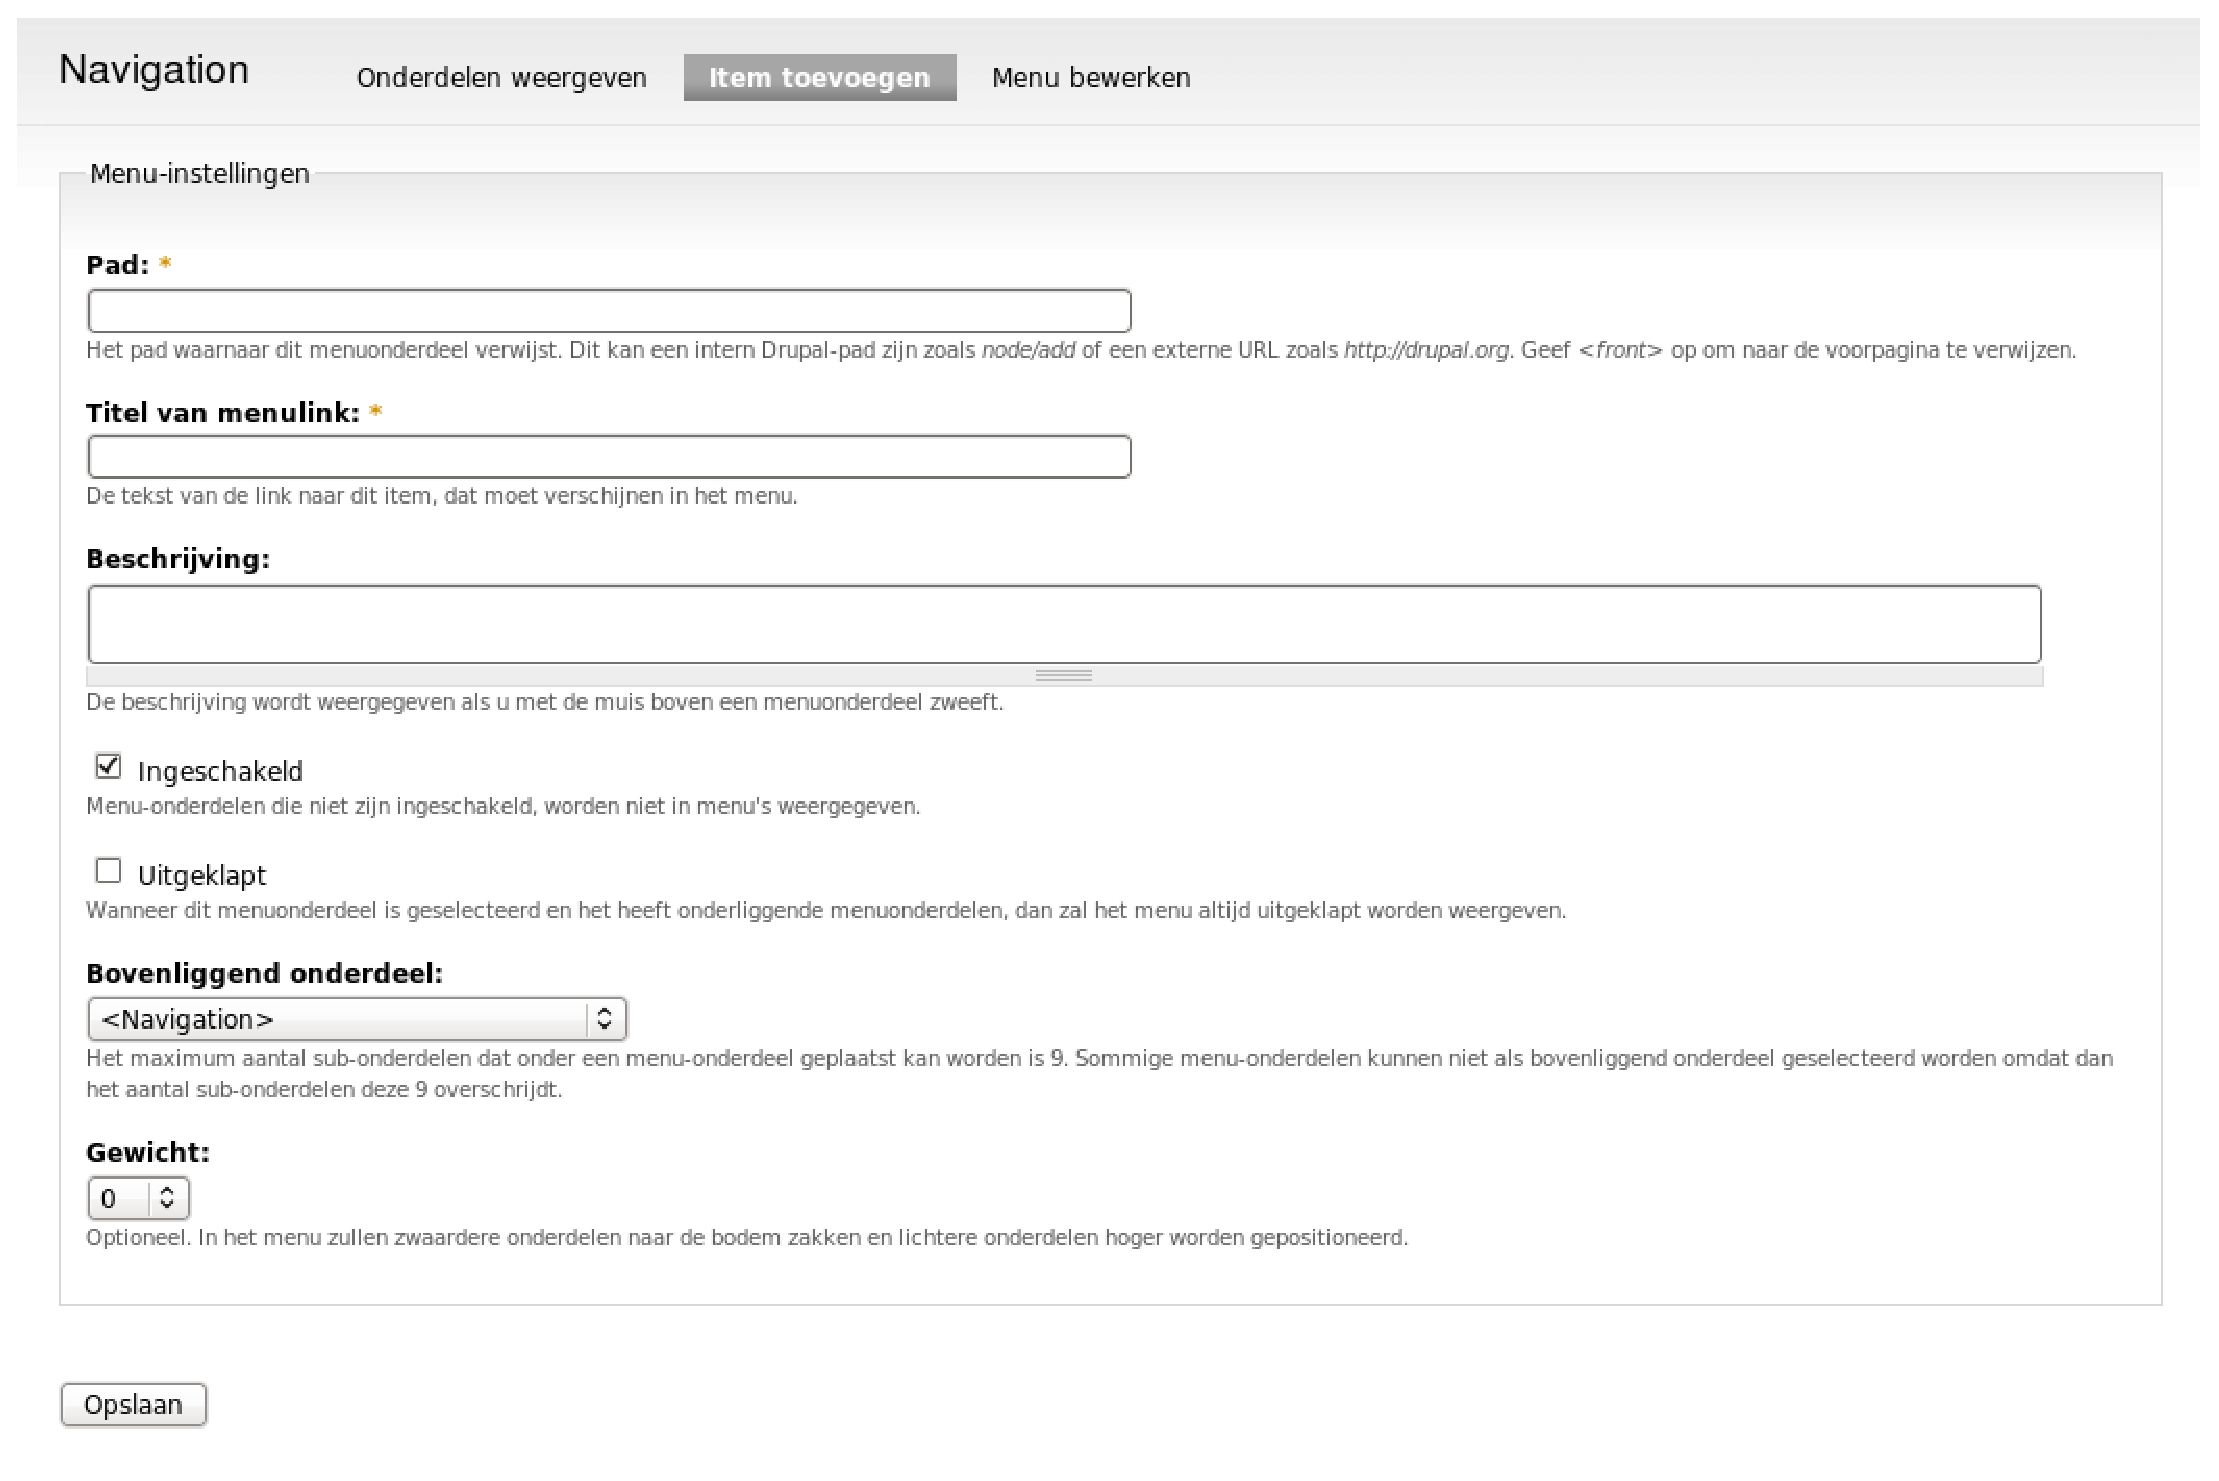
\includegraphics[scale=0.3,angle=0]{nav-item-toevoegen}
%    \caption{nav-item-toevoegen.\label{white}}
%  \end{figure}
%  \subsubsection{Menu bewerken}
%  \begin{figure}[!h]
%     \centering
%    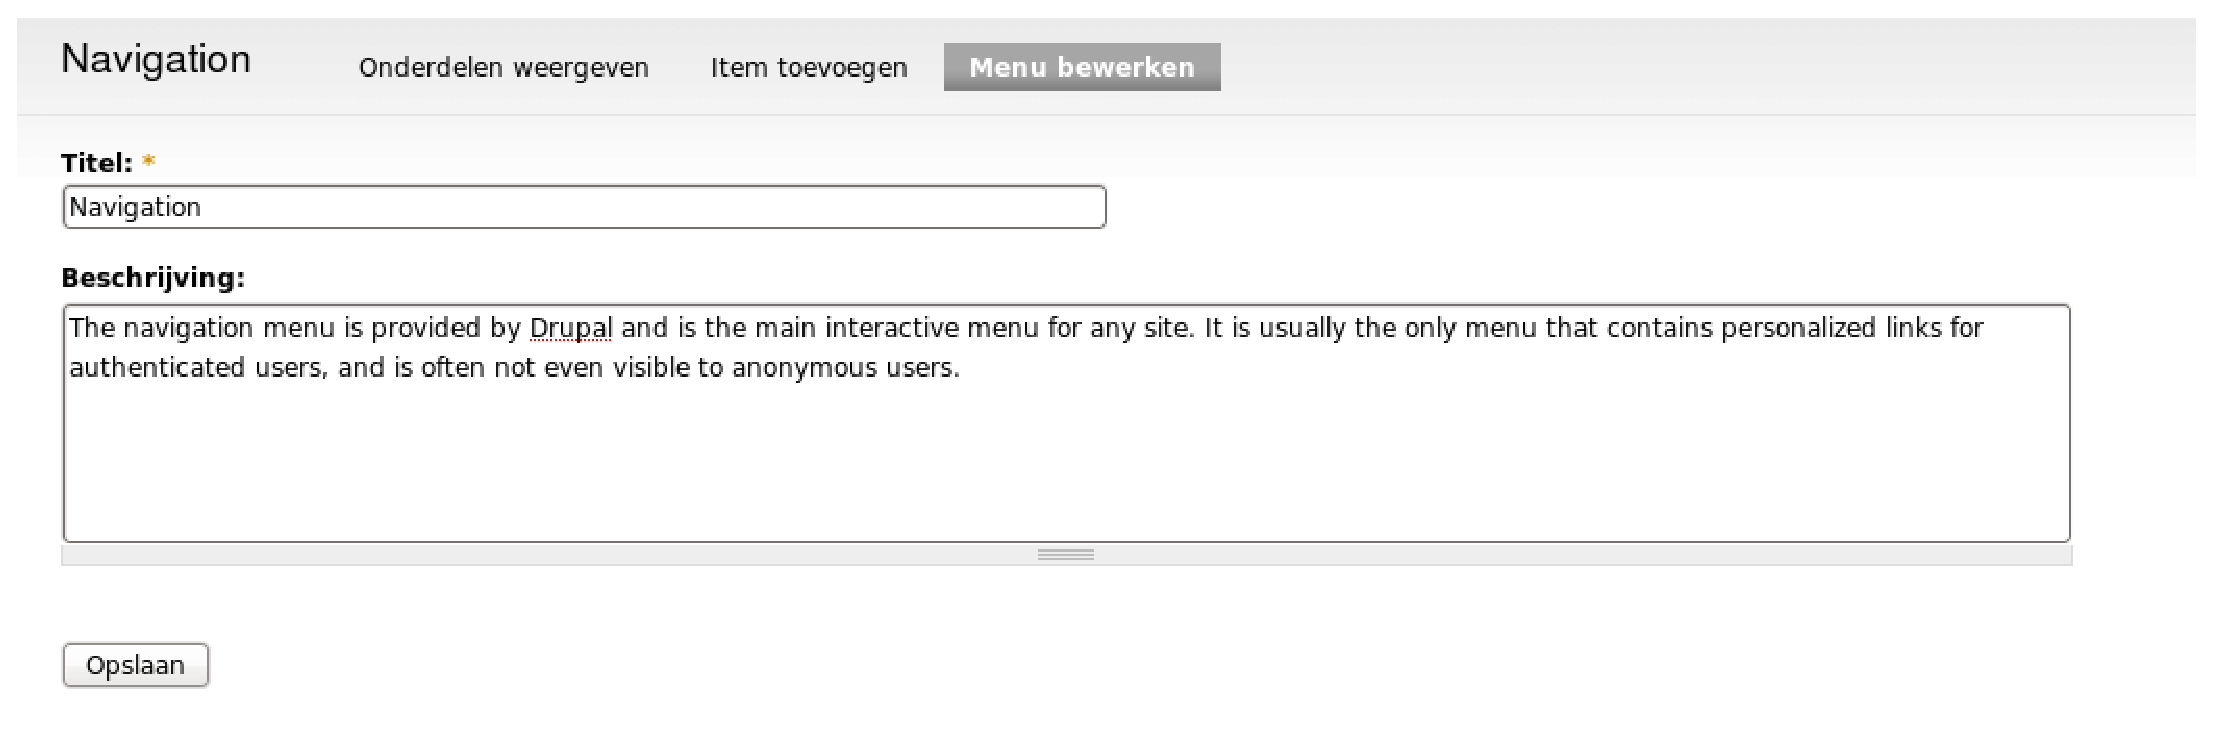
\includegraphics[scale=0.3,angle=0]{nav-menu-bewerken}
%    \caption{nav-menu-bewerken.\label{white}}
%  \end{figure}



\section{Modules} \index{modules}
Modules zijn plugins \index{plugins} voor Drupal die de kernfunctionaliteit
uitbreiden.
\subsection{Module lijst}
Hier kunt u de ingeschakelde 
modules kiezen. Klik in het navigatiemenu op de naam van de module voor de betreffende instellingenpagina. 
Als een module eenmaal is ingeschakeld kunnen nieuwe toegangsrechten beschikbaar zijn. 
Met behulp van de Throttle-module \index{throttle-module} kunnen modules
automatisch tijdelijk worden uitgeschakeld om de belasting van de server te verminderen op momenten dat de site extreem druk wordt bezocht.
\\
Het is belangrijk om update.php uit te voeren nadat een nieuwere versie van een
module is ge\"installeerd.
\\
U kunt alle beheertaken van een bepaalde module vinden op de pagina beheer per module.
\begin{figure}[!h]
    \centering
   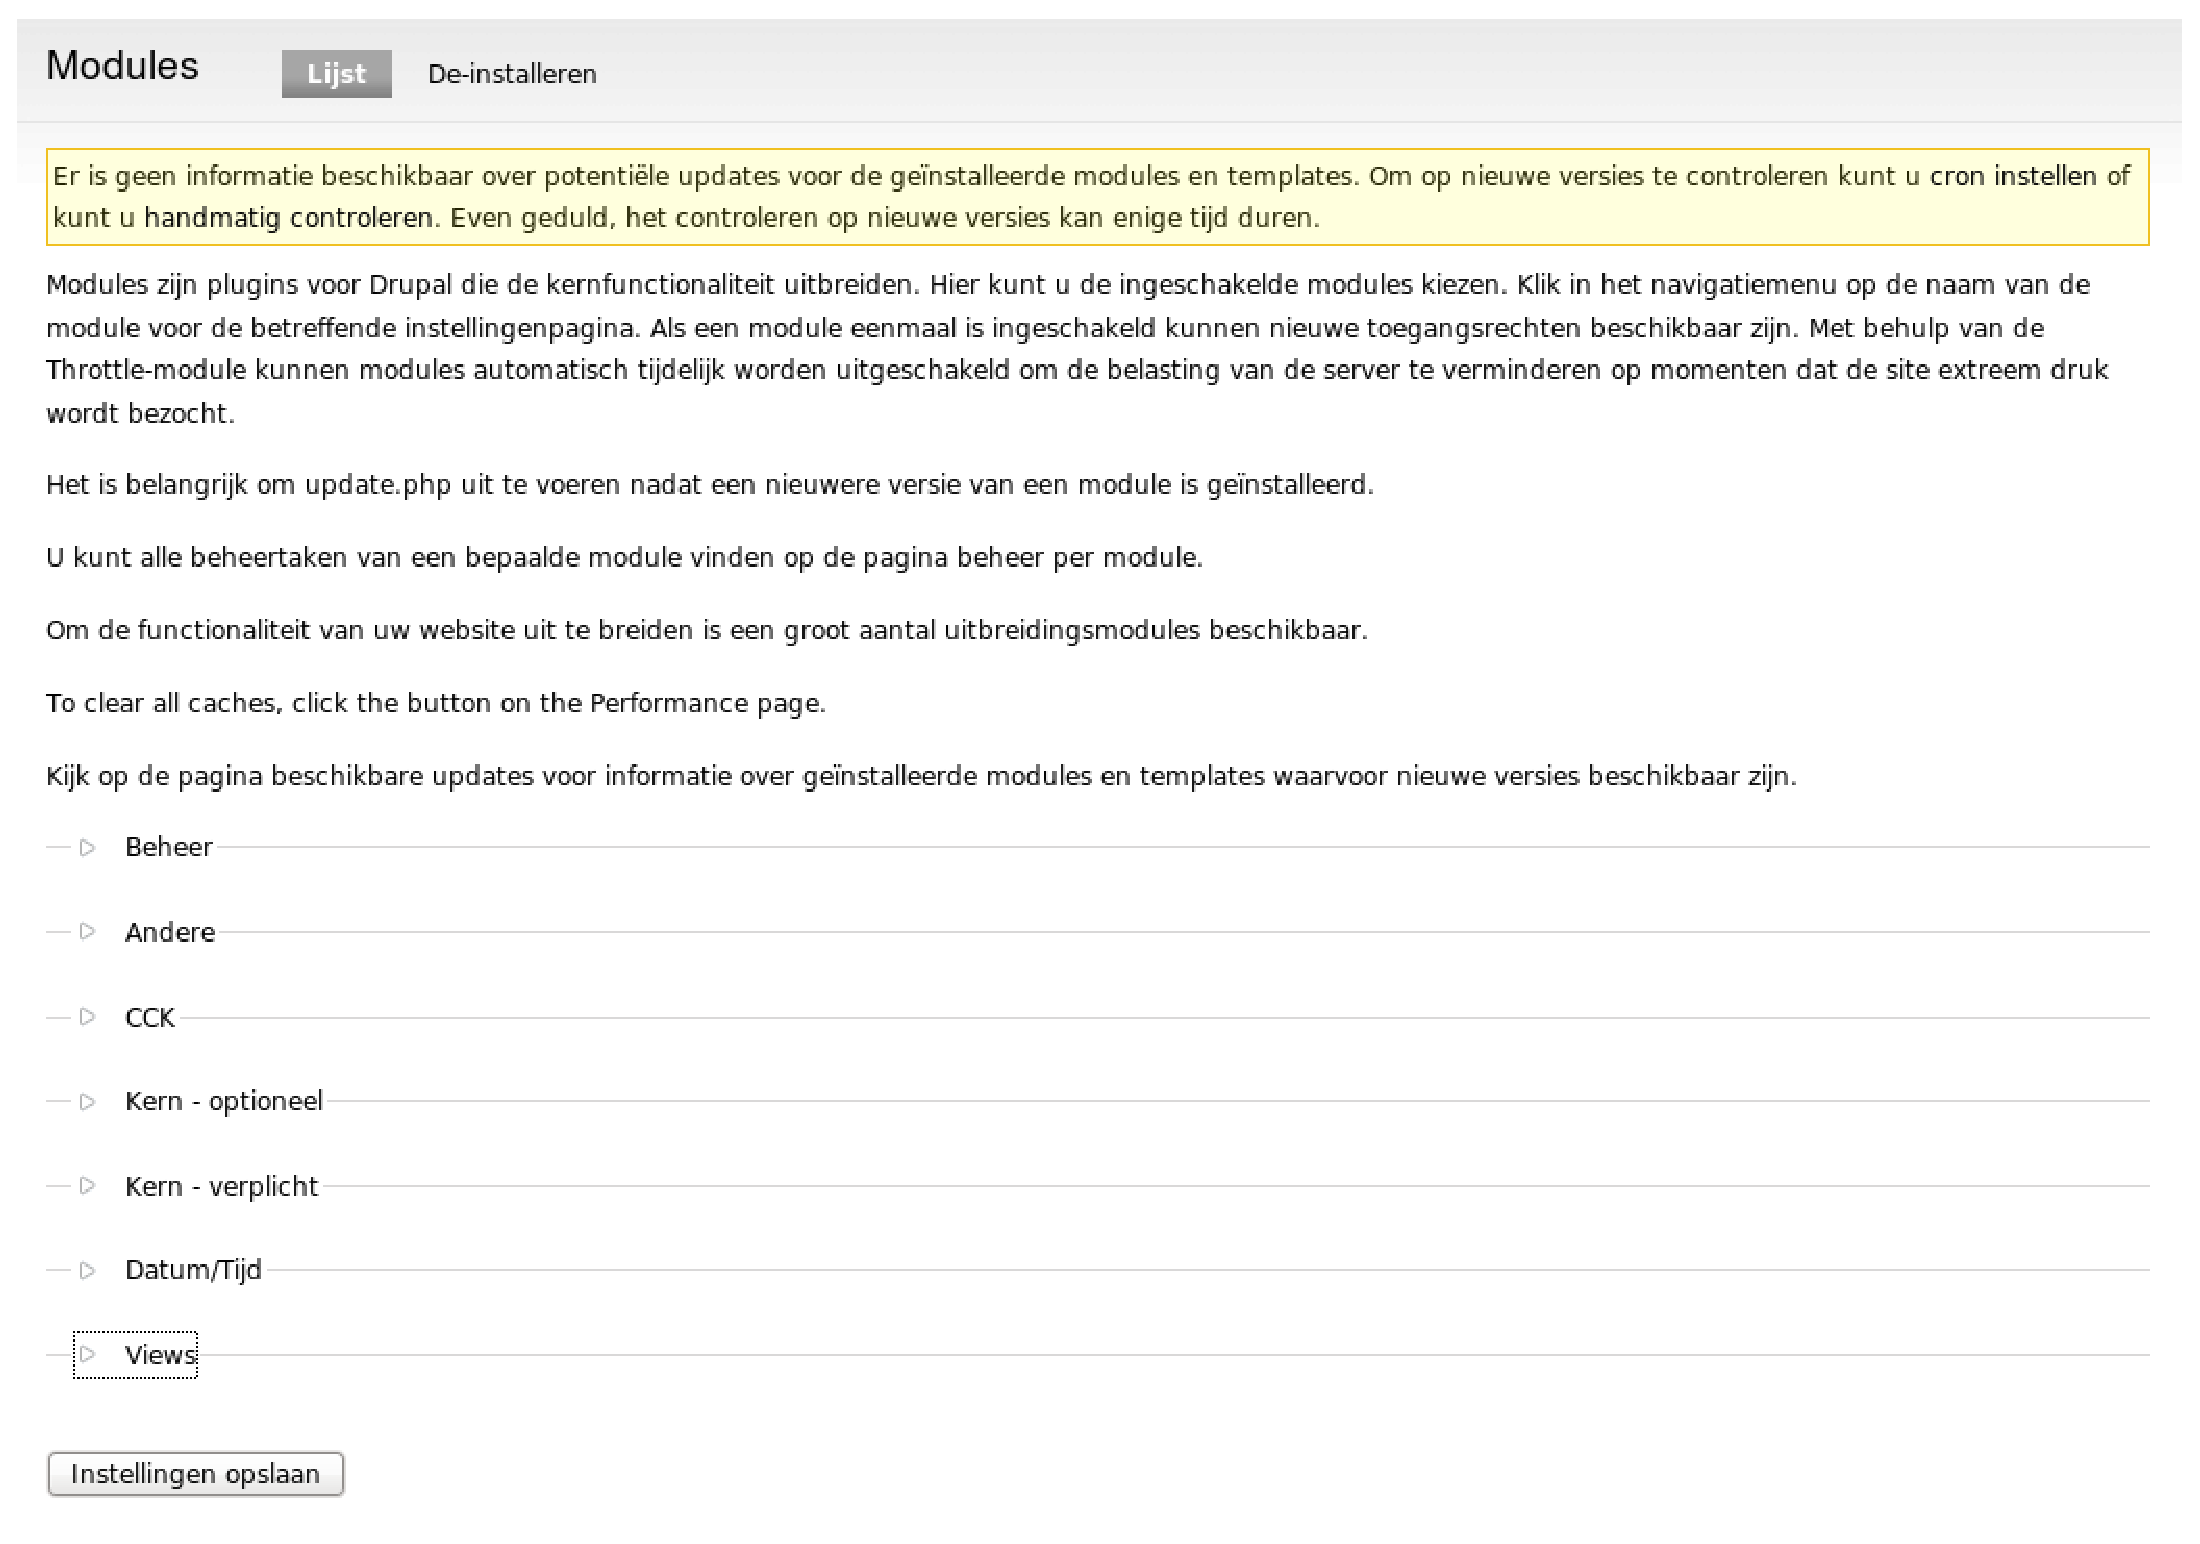
\includegraphics[scale=0.3,angle=0]{modules-lijst}
   \caption{modules-lijst.\label{white}}
 \end{figure}
 Om de functionaliteit van uw website uit te breiden is een groot aantal
 uitbreidingsmodules beschikbaar.
 
 
\subsection{Modules de-installeren} \index{de-installeren modules}
Het de-installatie proces verwijdert alle gegevens aan een module gerelateerde
gegevens. Schakel een module eerst uit, alvorens deze te de-installeren. De-installatie wordt niet door alle modules ondersteund.
\begin{figure}[!h]
    \centering
   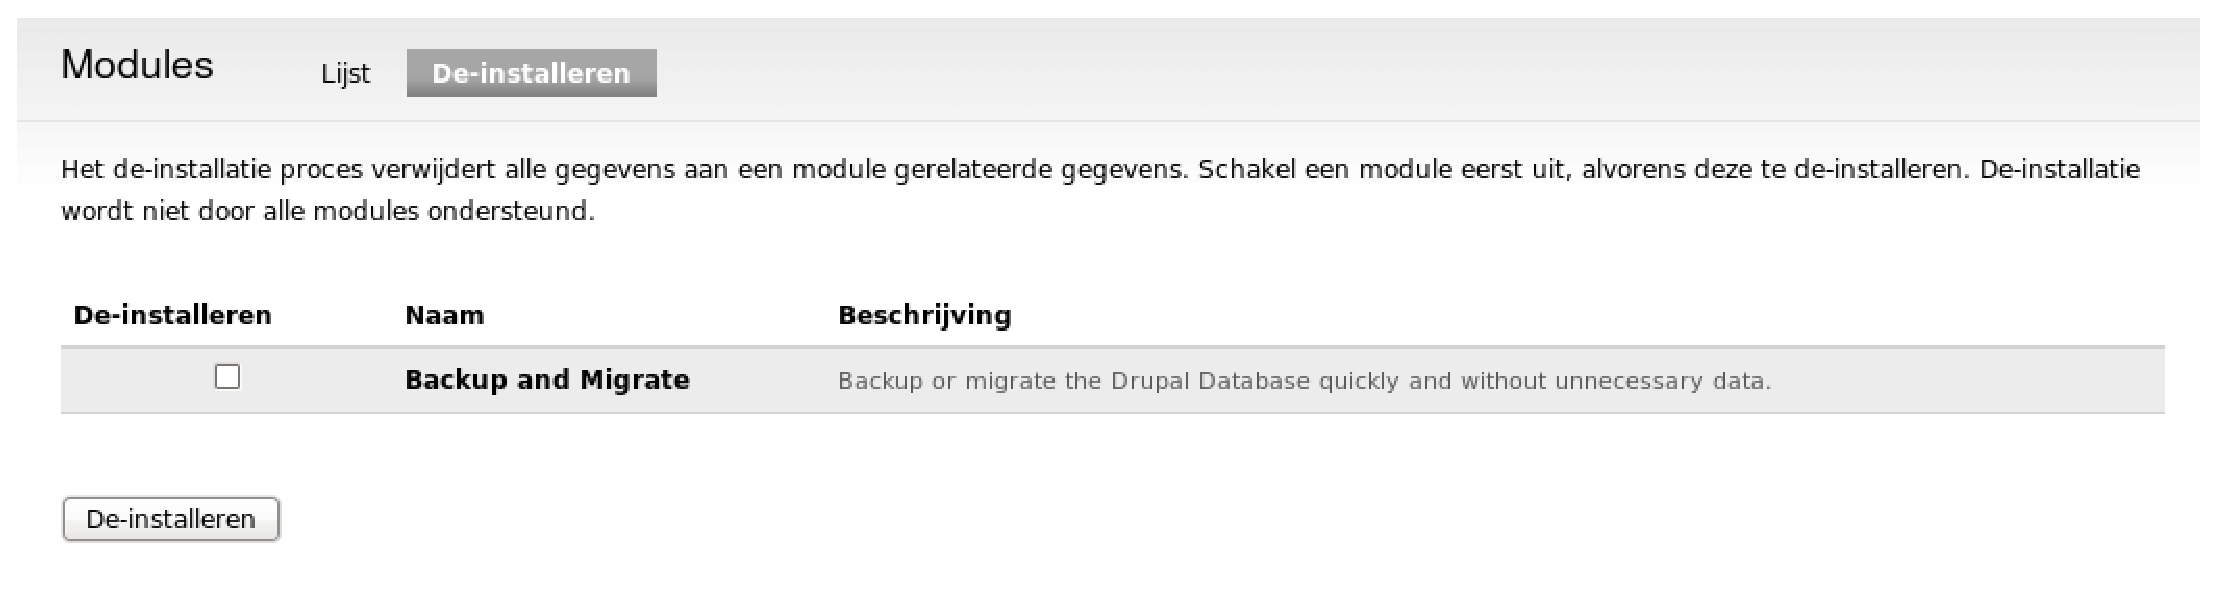
\includegraphics[scale=0.3,angle=0]{modules-deinstalleren}
   \caption{modules-deinstalleren.\label{white}}
 \end{figure}

\section{Templates} \index{templates}
De template voor de weergave van de site bepalen of deze keuze aan de gebruikers
laten. Om het uiterlijk van uw website te veranderen zijn er diverse
uitbreidingstemplates beschikbaar.

\subsection{Templates lijst}
Selecteer de templates die voor uw gebruikers beschikbaar zijn en stel een
standaard template in. Klik voor algemene weergave-instellingen op de Link 'instellen' hierboven. 
Klik op de link voor het betreffende template waarvoor u deze instellingen wilt wijzigen. 
Let er op dat verschillende templates verschillende regionen voor weergave van inhoud kunnen hebben; 
voor consistentie in de presentatie kunt u het best slechts \'e\'en template
inschakelen. \begin{figure}[!h]
    \centering
   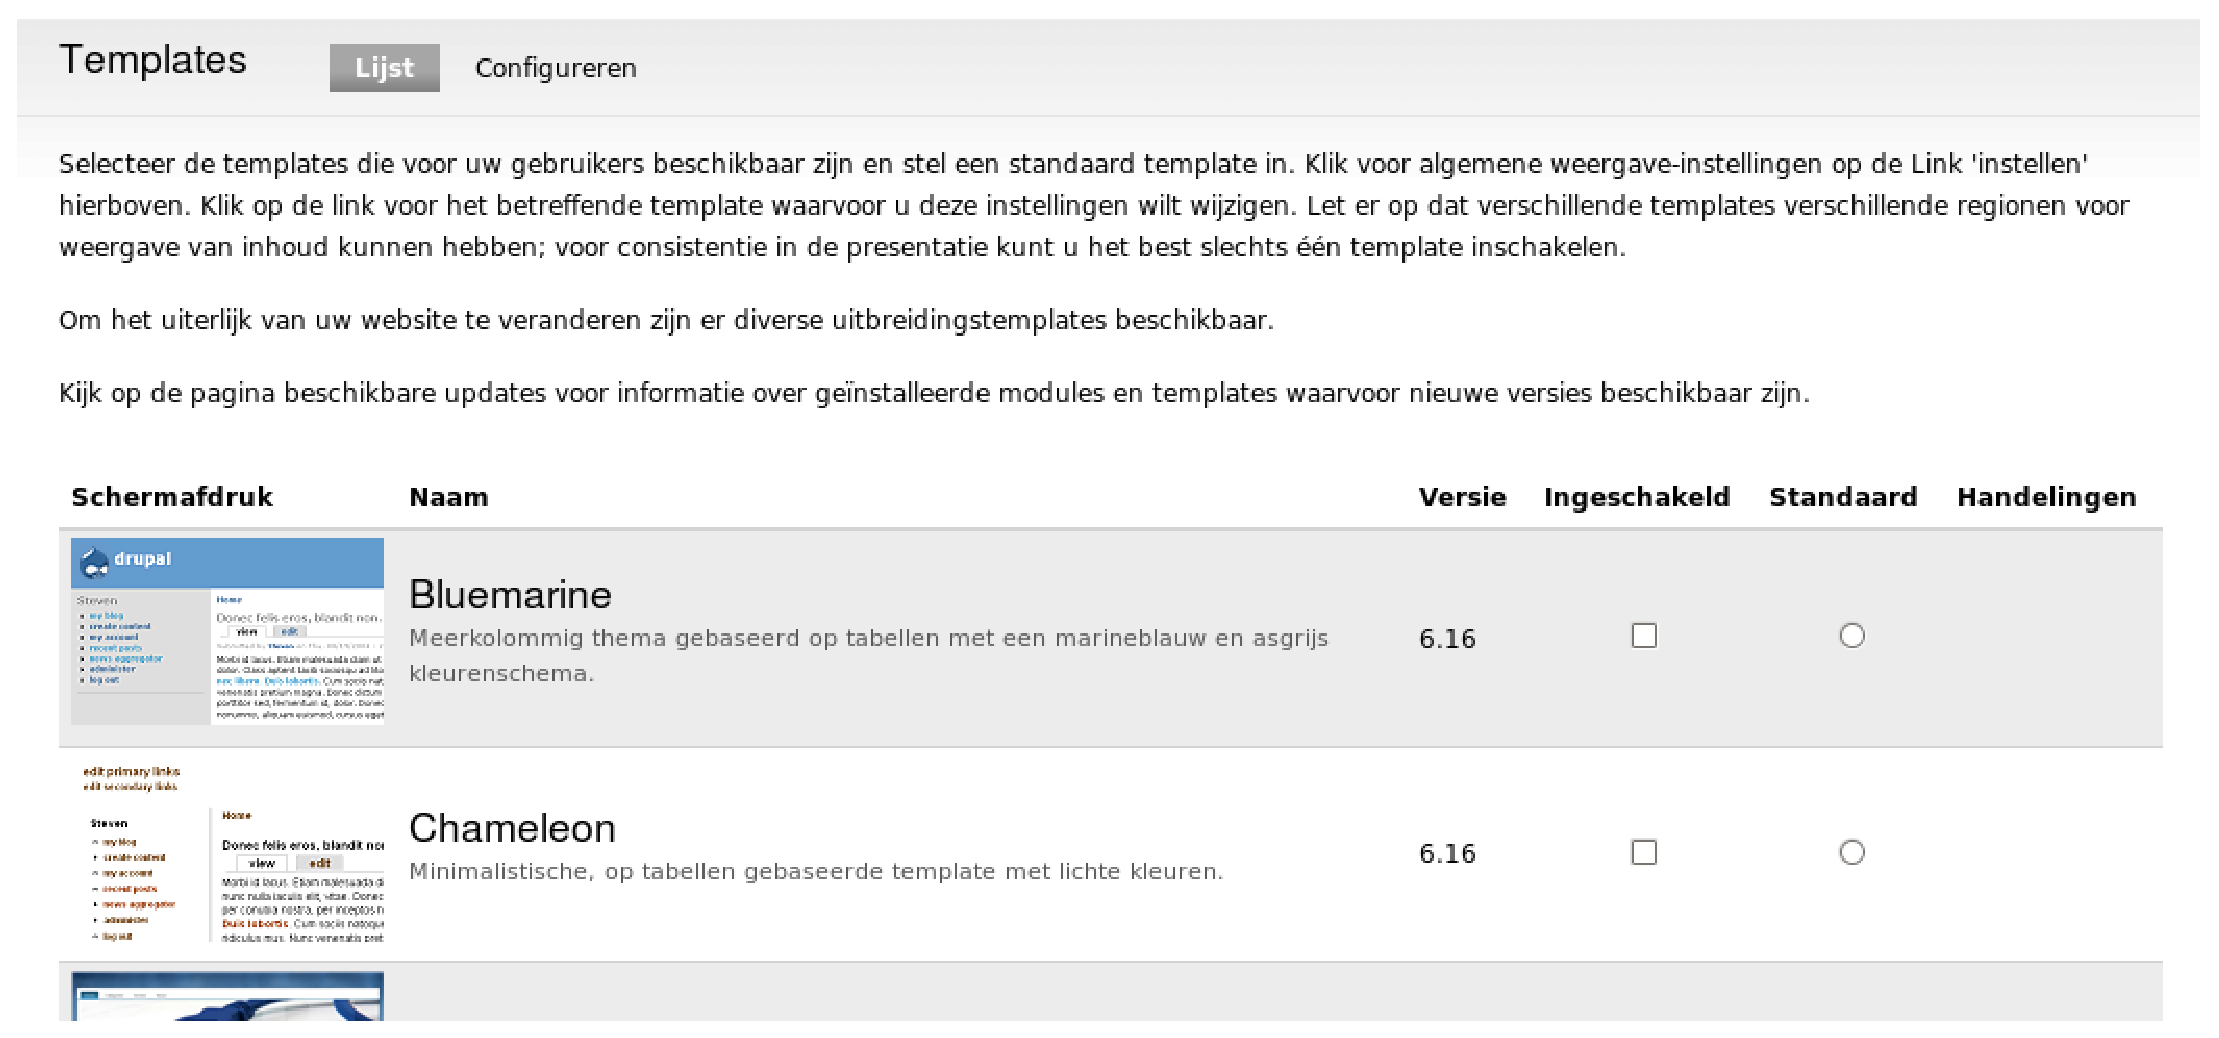
\includegraphics[scale=0.3,angle=0]{templates-lijst}
   \caption{templates-lijst.\label{white}}
 \end{figure}
 
 \subsection{Configureren globale instellingen} \index{globale instellingen}
 Deze opties sturen de standaard weergave-instellingen voor uw volledige website
 voor alle templates. Tenzij deze teniet gedaan worden door een specifieke template, zullen deze instellingen gebruikt worden.
 \begin{figure}[!h]
    \centering
   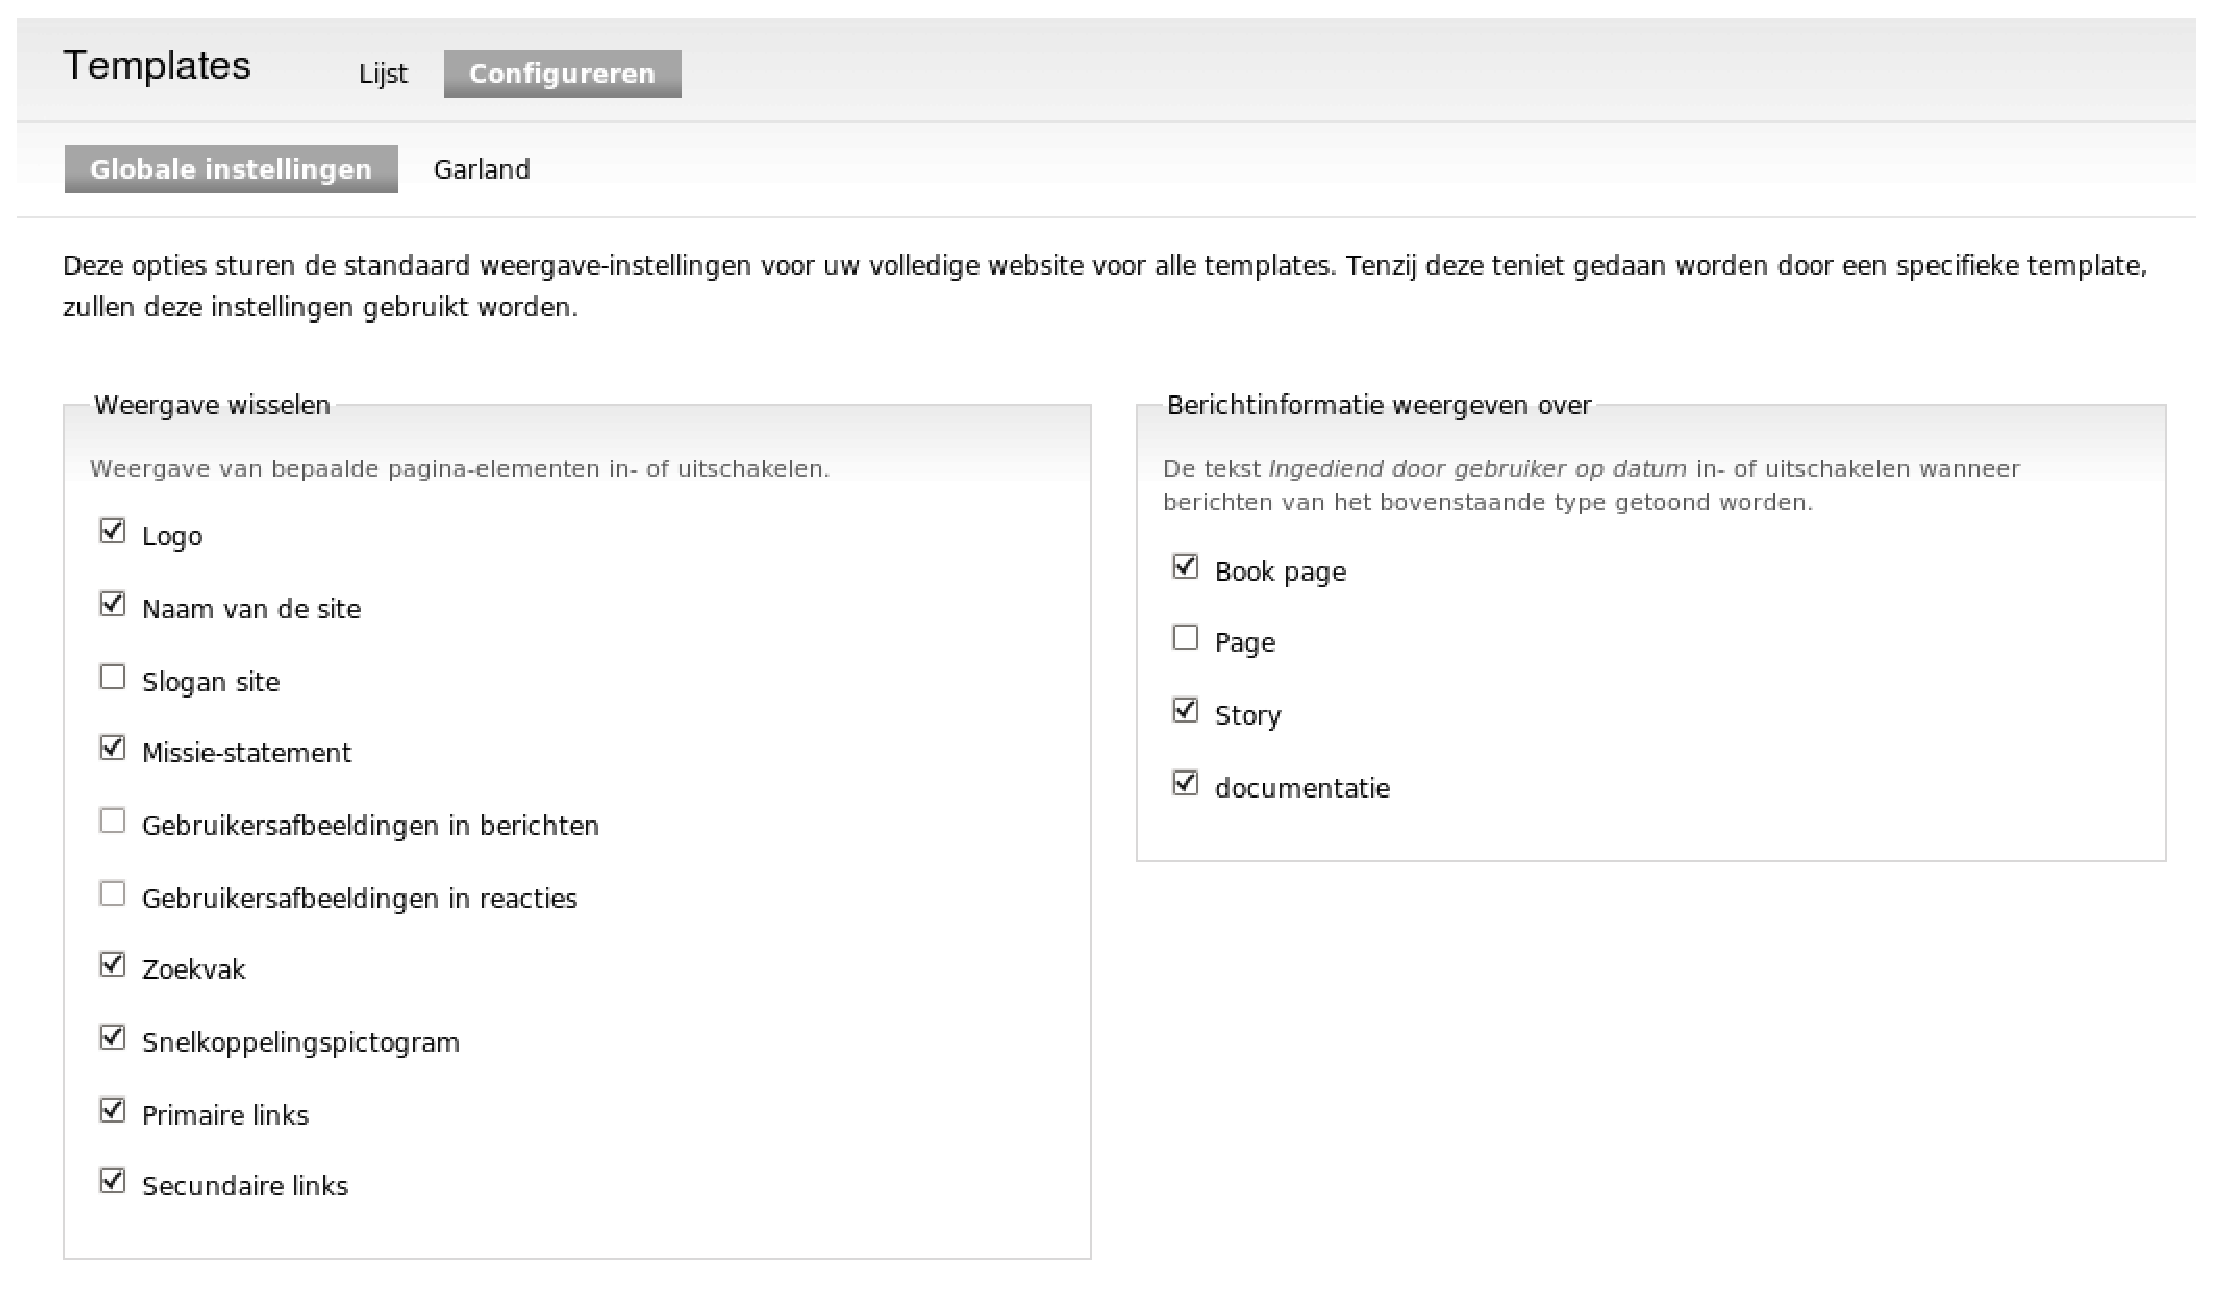
\includegraphics[scale=0.3,angle=0]{templates-globale-instellingen}
   \caption{templates-globale-instellingen.\label{white}}
 \end{figure}
 
\subsection{Configureren specifieke template instellingen} 
Deze opties bepalen de weergave-instellingen van de garland-template. Wanneer uw
website met deze template wordt weergegeven, zullen deze instellingen gebruikt worden. Door op "Standaardwaarden terugzetten" te klikken, 
kunt u de globale instellingen voor deze template gebruiken.
 \begin{figure}[!h]
    \centering
   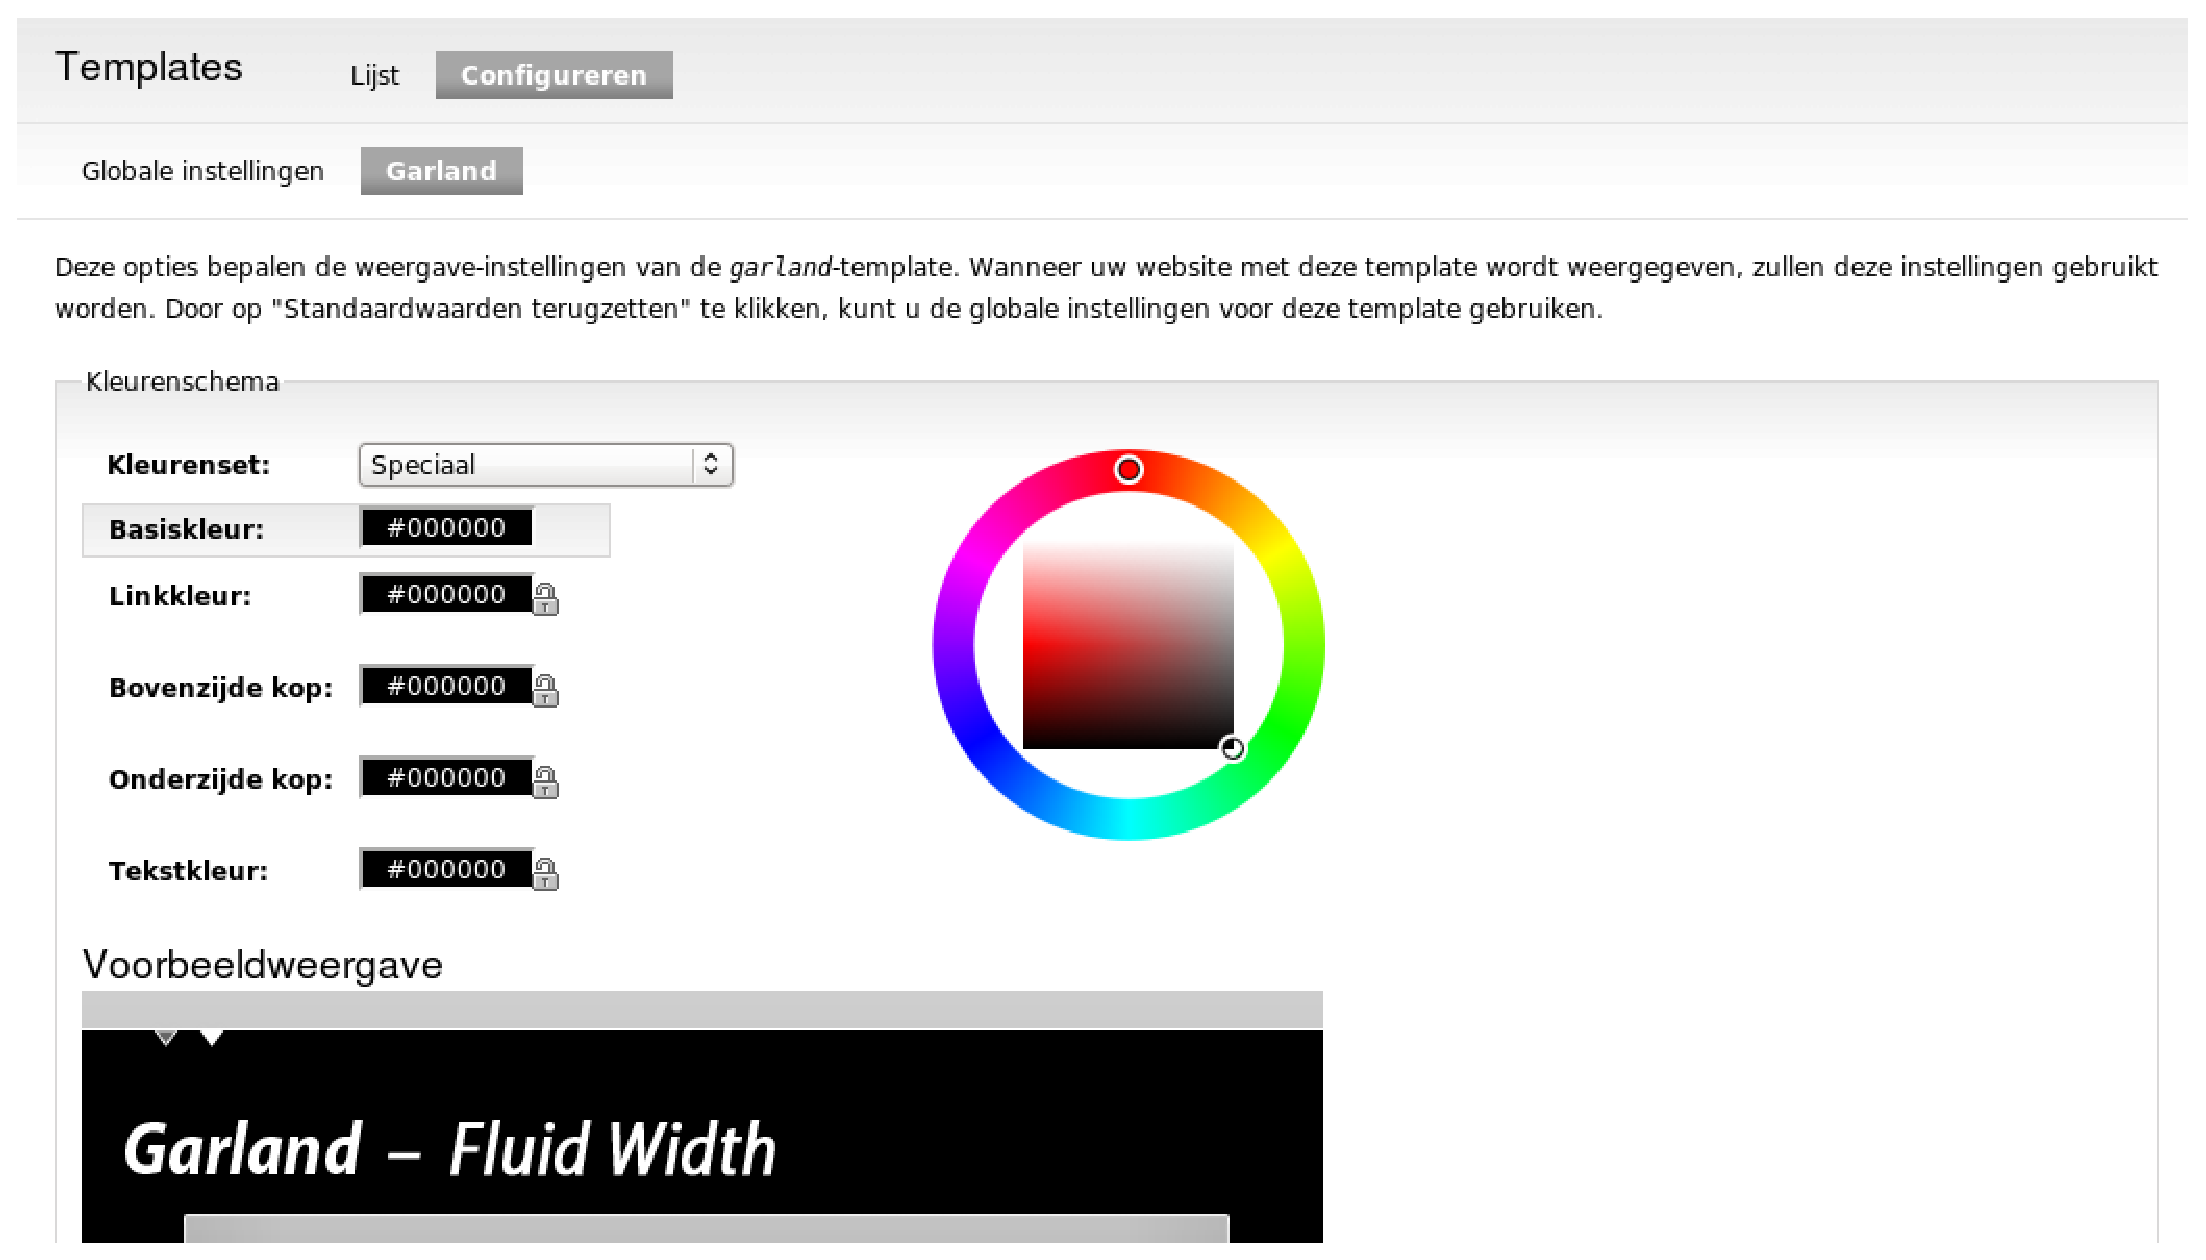
\includegraphics[scale=0.3,angle=0]{templates-garland}
   \caption{templates-garland.\label{white}}
 \end{figure}
 
\section{URL-aliassen} \index{aliassen}
De URL-paden van de site met behulp van aliassen wijzigen.

\subsection{URL-aliassen lijst}
Drupal biedt volledige controle over URL's door het gebruik van aliassen. 
Deze voorziening wordt meestal gebruikt om URL's makkelijker leesbaar te maken 
of eenvoudiger te herinneren. Zo kan men bijvoorbeeld het systeempad 'node/1' verbinden aan 'over-ons' en 
zo de URL een betekenis geven. Elk systeempad kan aan meerdere aliassen gekoppeld zijn.
 \begin{figure}[!h]
    \centering
   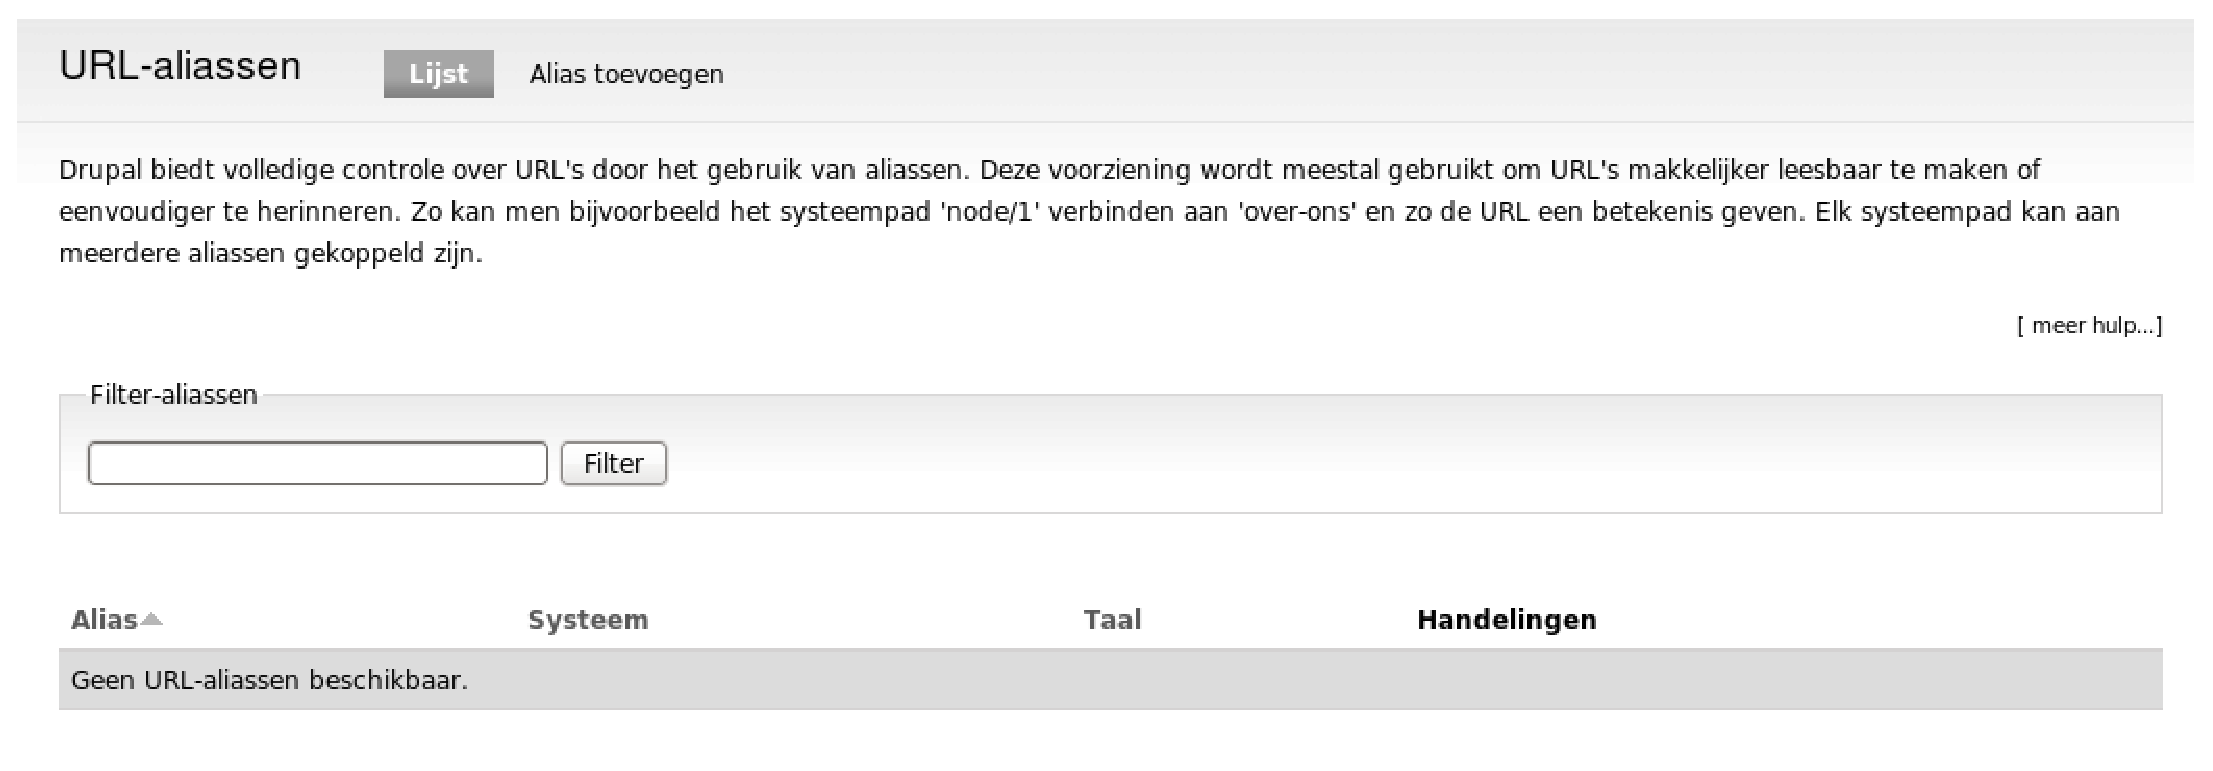
\includegraphics[scale=0.3,angle=0]{url-aliassen-lijst}
   \caption{url-aliassen-lijst.\label{white}}
 \end{figure}
 
\subsection{Alias toevoegen}
 Voer het pad in waarvoor u een alias wenst te cre\"eren, gevolgd door de naam
 van het nieuwe alias.
 \begin{figure}[!h]
    \centering
   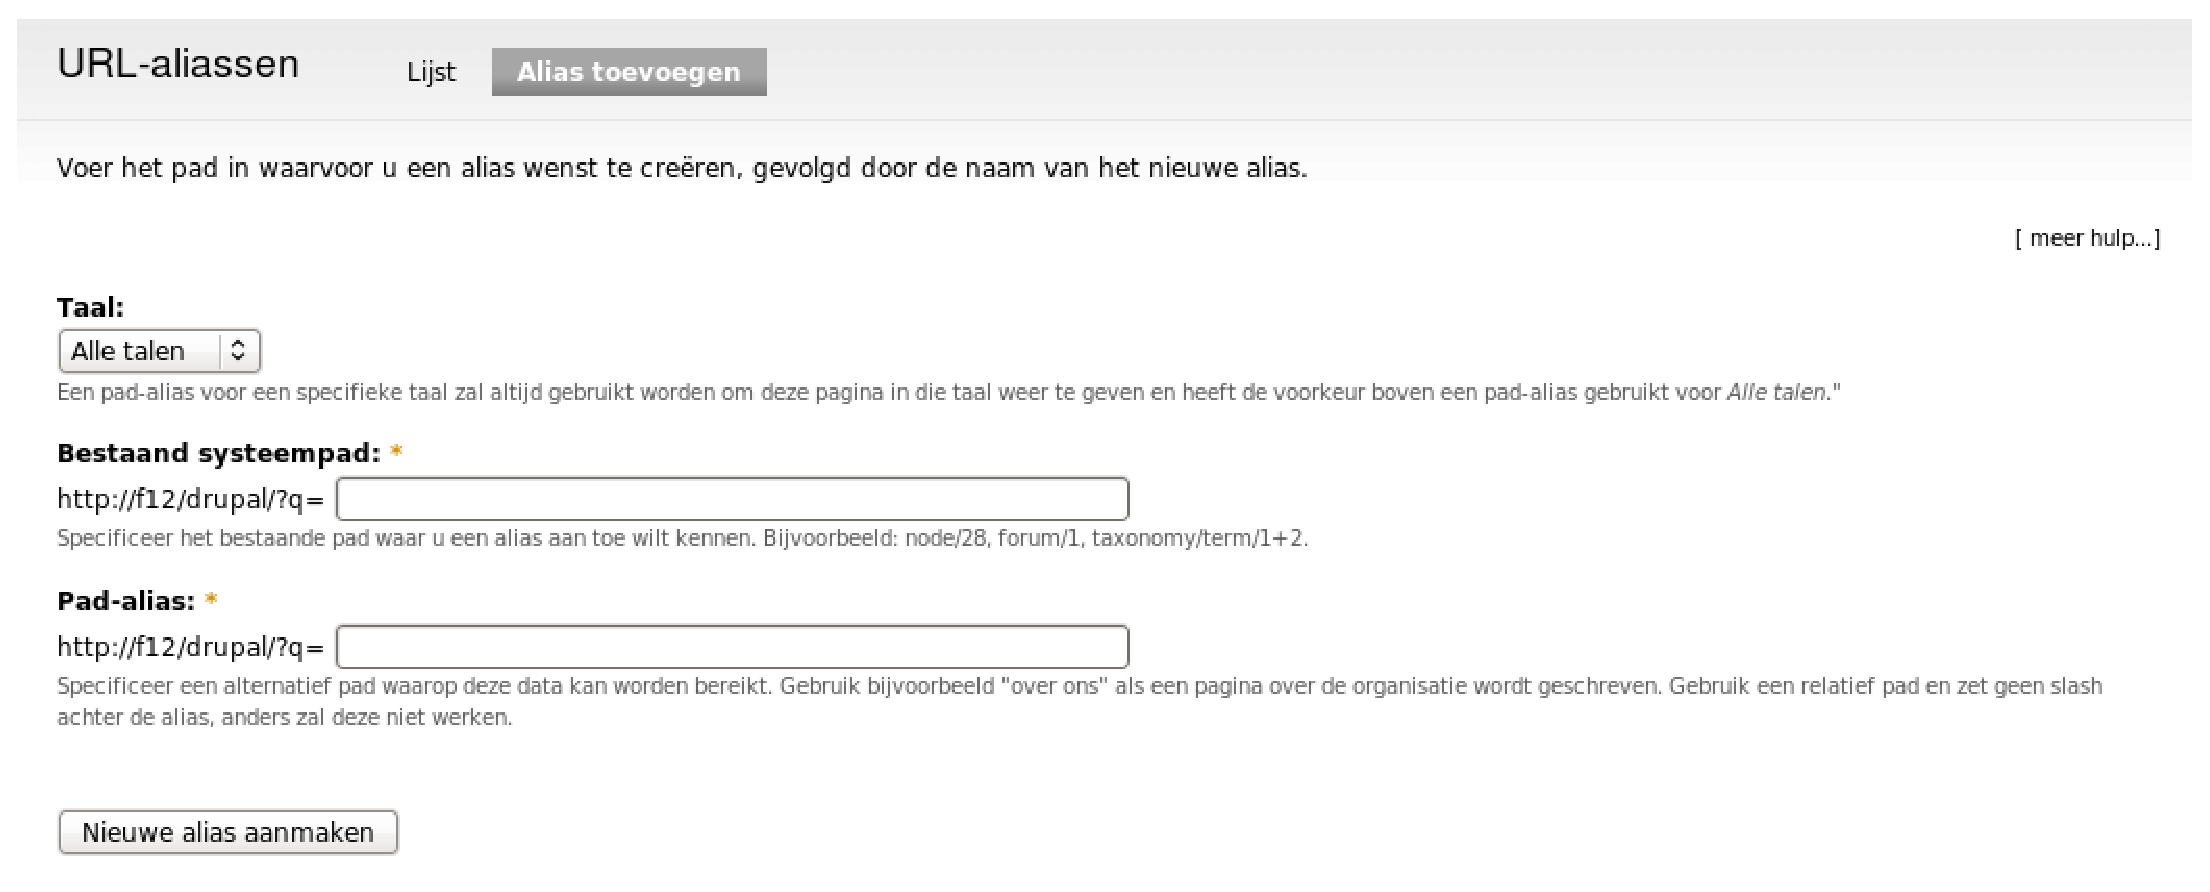
\includegraphics[scale=0.3,angle=0]{url-alias-toevoegen}
   \caption{url-alias-toevoegen.\label{white}}
 \end{figure}
 
\subsection{Path-module} \index{path-module}
Met de Path-module kunt u aliassen voor Drupal-URL's worden opgeven. 
Aliassen verbeteren de leesbaarheid van URL's voor gebruikers en kunnen 
zoekmachines helpen de pagina's effectiever te indexeren. Per pagina mogen meerdere aliassen worden opgegeven.
\\
Enkele voorbeelden van URL-aliassen:
\begin{itemize}
\item user/login $\Rightarrow$ login
\item image/tid/16 $\Rightarrow$ store
\item taxonomy/term/7+19+20+21 $\Rightarrow$ store/products/whirlygigs
\item node/3 $\Rightarrow$ contact
\end{itemize}
Met de Path-module kunnen gebruikers met de juiste toegangsrechten een alias opgeven bij het toevoegen 
of wijzigen van een pagina en het biedt een interface om de aliassen op de site te beheren. 
Twee toegangsrechten die met URL-aliassen samenhangen zijn URL-aliassen beheren en URL-aliassen aanmaken.
\\
De Path-module beschikt ook over de mogelijkheid om volgens eigen specificatie massaal URL-aliassen 
toe te wijzen. Hiermee kunt u eigen uniforme URL's toegepassen, bijvoorbeeld: URL's in een andere taal 
weergeven. Server-toegang tot de Drupal-broncode is nodig om dit soort URL's te realiseren. 

blabla
%  \chapter{Site-instellingen}
\section{Actions}

Acties zijn individuele taken die door het systeem uitgevoerd kunnen worden, zoals publicatie 
van een pagina ongedaan maken of uitsluiten van een gebruiker. Modules, zoals de
Trigger-module, \index{trigger-module} kunnen deze acties starten wanneer
bepaalde systeemgebeurtennissen plaatsvinden; bijvoorbeeld wanneer een nieuw bericht wordt toegevoegd of wanneer een gebruiker inlogt. Modules kunnen 
voorzien in extra acties.
\\
Er zijn twee soorten acties: eenvoudige en geavanceerde. Eenvoudige acties behoeven geen extra 
configuratie en worden hier automatisch opgesomd. Geavanceerde acties kunnen meer dan eenvoudige 
acties, bijvoorbeeld een e-mail versturen naar een gespecificeerd adres, of inhoud controleren 
op bepaalde woorden. Deze acties moeten eerst worden aangemaakt en geconfigureerd voordat ze 
gebruikt kunnen worden. Selecteer een actie uit het keuzelijstmenu en klik op de knop Aanmaken 
om een geavanceerde actie aan te maken.
\begin{figure}[!h]
    \centering
   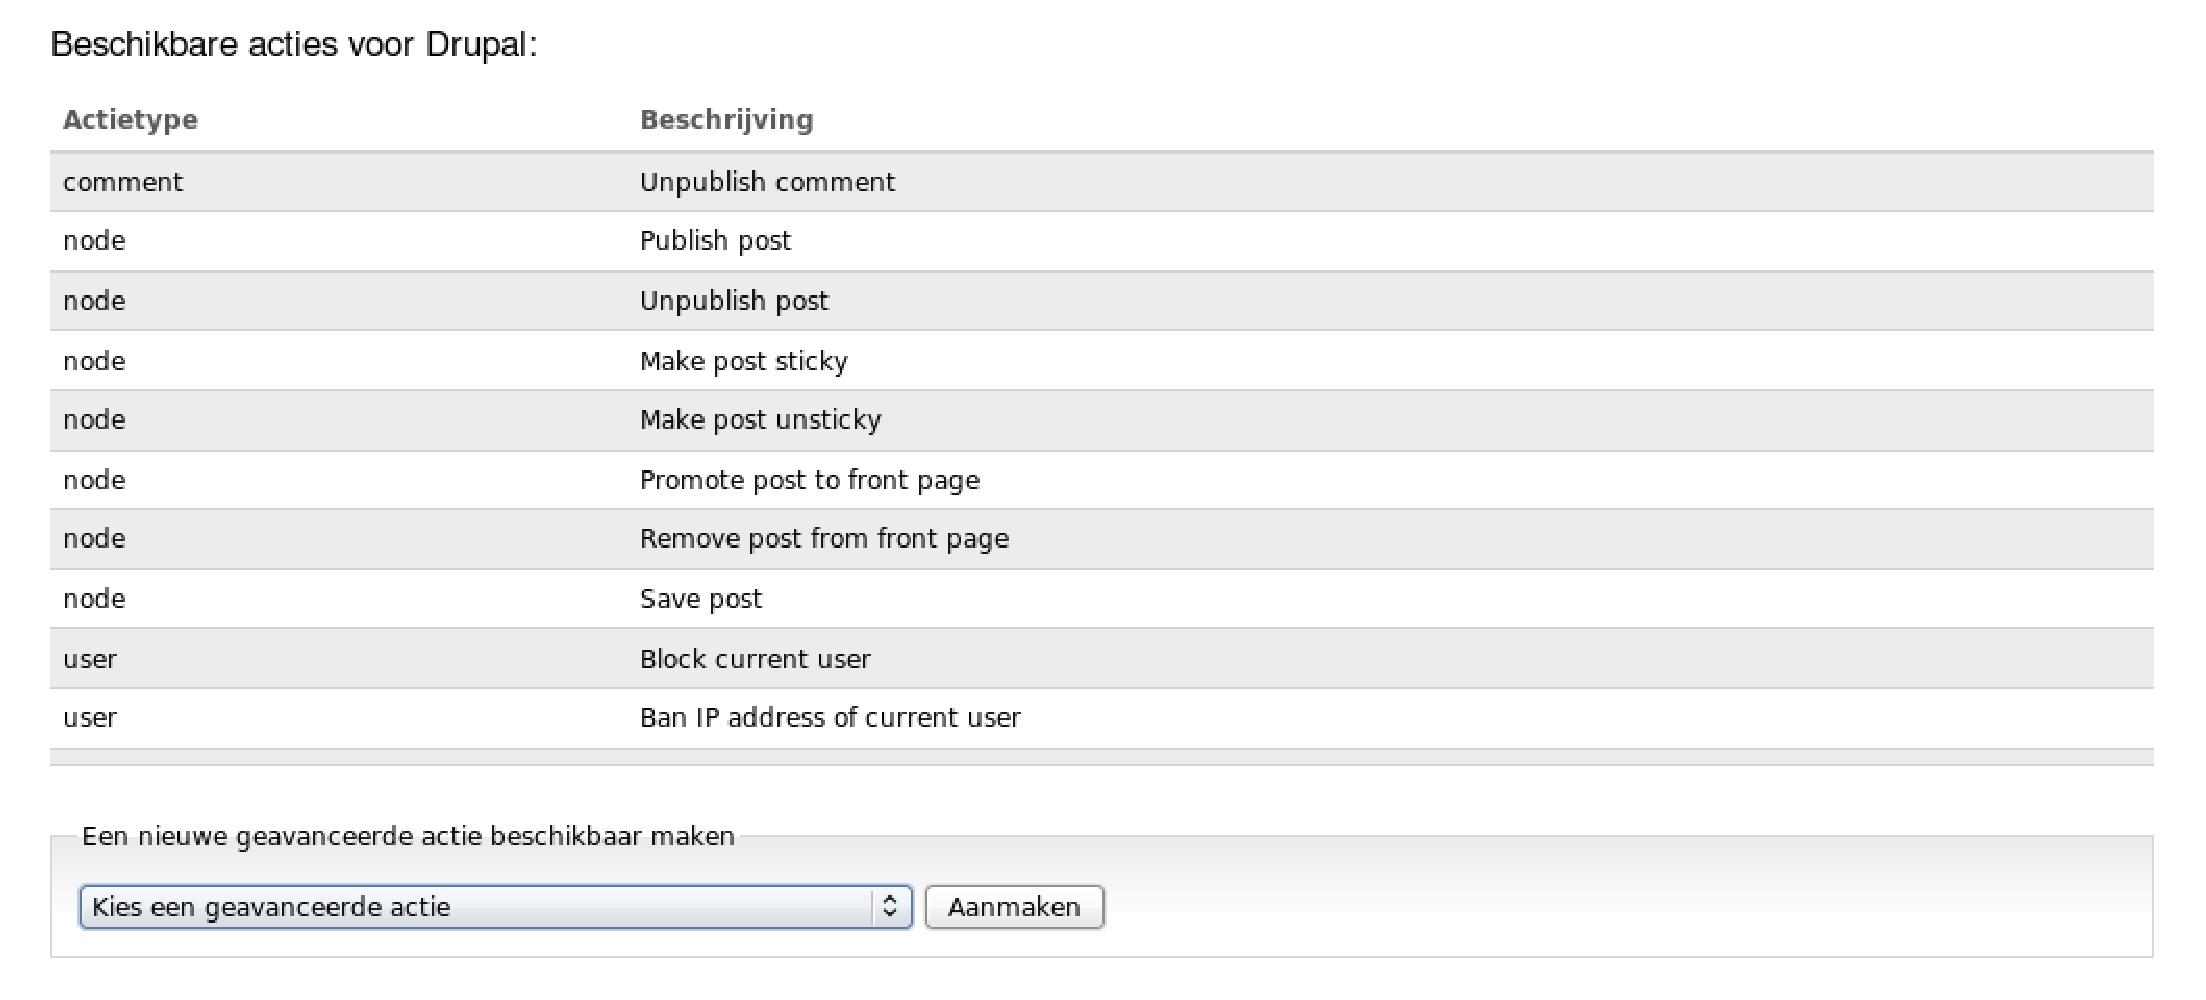
\includegraphics[scale=0.3,angle=0]{Actions}
   \caption{Actions.\label{white}}
 \end{figure}

\section{Administratiemenu} \index{administratiemenu}
De administratiemenu-module \index{administratiemenu-module} voorziet een
keuzelijstmenu dat met \'e\'en of twee klikken toegang biedt tot de meeste beheertaken en andere gemeenschappelijke bestemmingen (aan gebruikers met de gepaste 
toegangsrechten). Het administratiemenu toont eveneens het aantal anonieme en geverifieerde gebruikers 
en laat toe dat modules hun eigen menu-onderdelen toevoegen. Integratie van het menu hangt af van 
module tot module; bijvoorbeeld de uitbreidingsmodule Devel, maakt veel gebruik van de 
administratiemenu-module om snel toegang te geven tot de ontwikkelingshulpmiddelen.
\\
De Instellingenpagina van het admnistratiemenu laat toe om sommige onderdelen van het gedrag en het 
voorkomen van het menu te veranderen. Vermits het voorkomen van het menu afhankelijk is van het 
thema van uw site, vereisen aanzienlijke aanpassingen ook wijzigingen aan de thema- en CSS-bestanden 
van uw site. 
\\
De menu-onderdelen die worden weergegeven in het administratiemenu hangen af van de toegangsrechten 
van de gebruiker. Ten eerste, het administratiemenu wordt alleen getoond aan gebruikers in 
rollen met het Toegang administratiemenu (admin-menu module) toegangsrecht. Ten
tweede, een gebruiker moet deel uitmaken van een rol met de Toegang tot beheerpagina's (system module) 
toegangsrecht om de administratieve linken te bekijken. Ten laatste, alleen de huidig toegelaten 
linken worden getoond; b.v. indien een gebruiker geen lid is van een rol met het toegangsrecht 
Toegangsrechten beheren (user module) en Gebruikers beheren (user module), wordt het 
Gebruikerbeheer menu-onderdeel niet getoond.
\begin{figure}[!h]
    \centering
   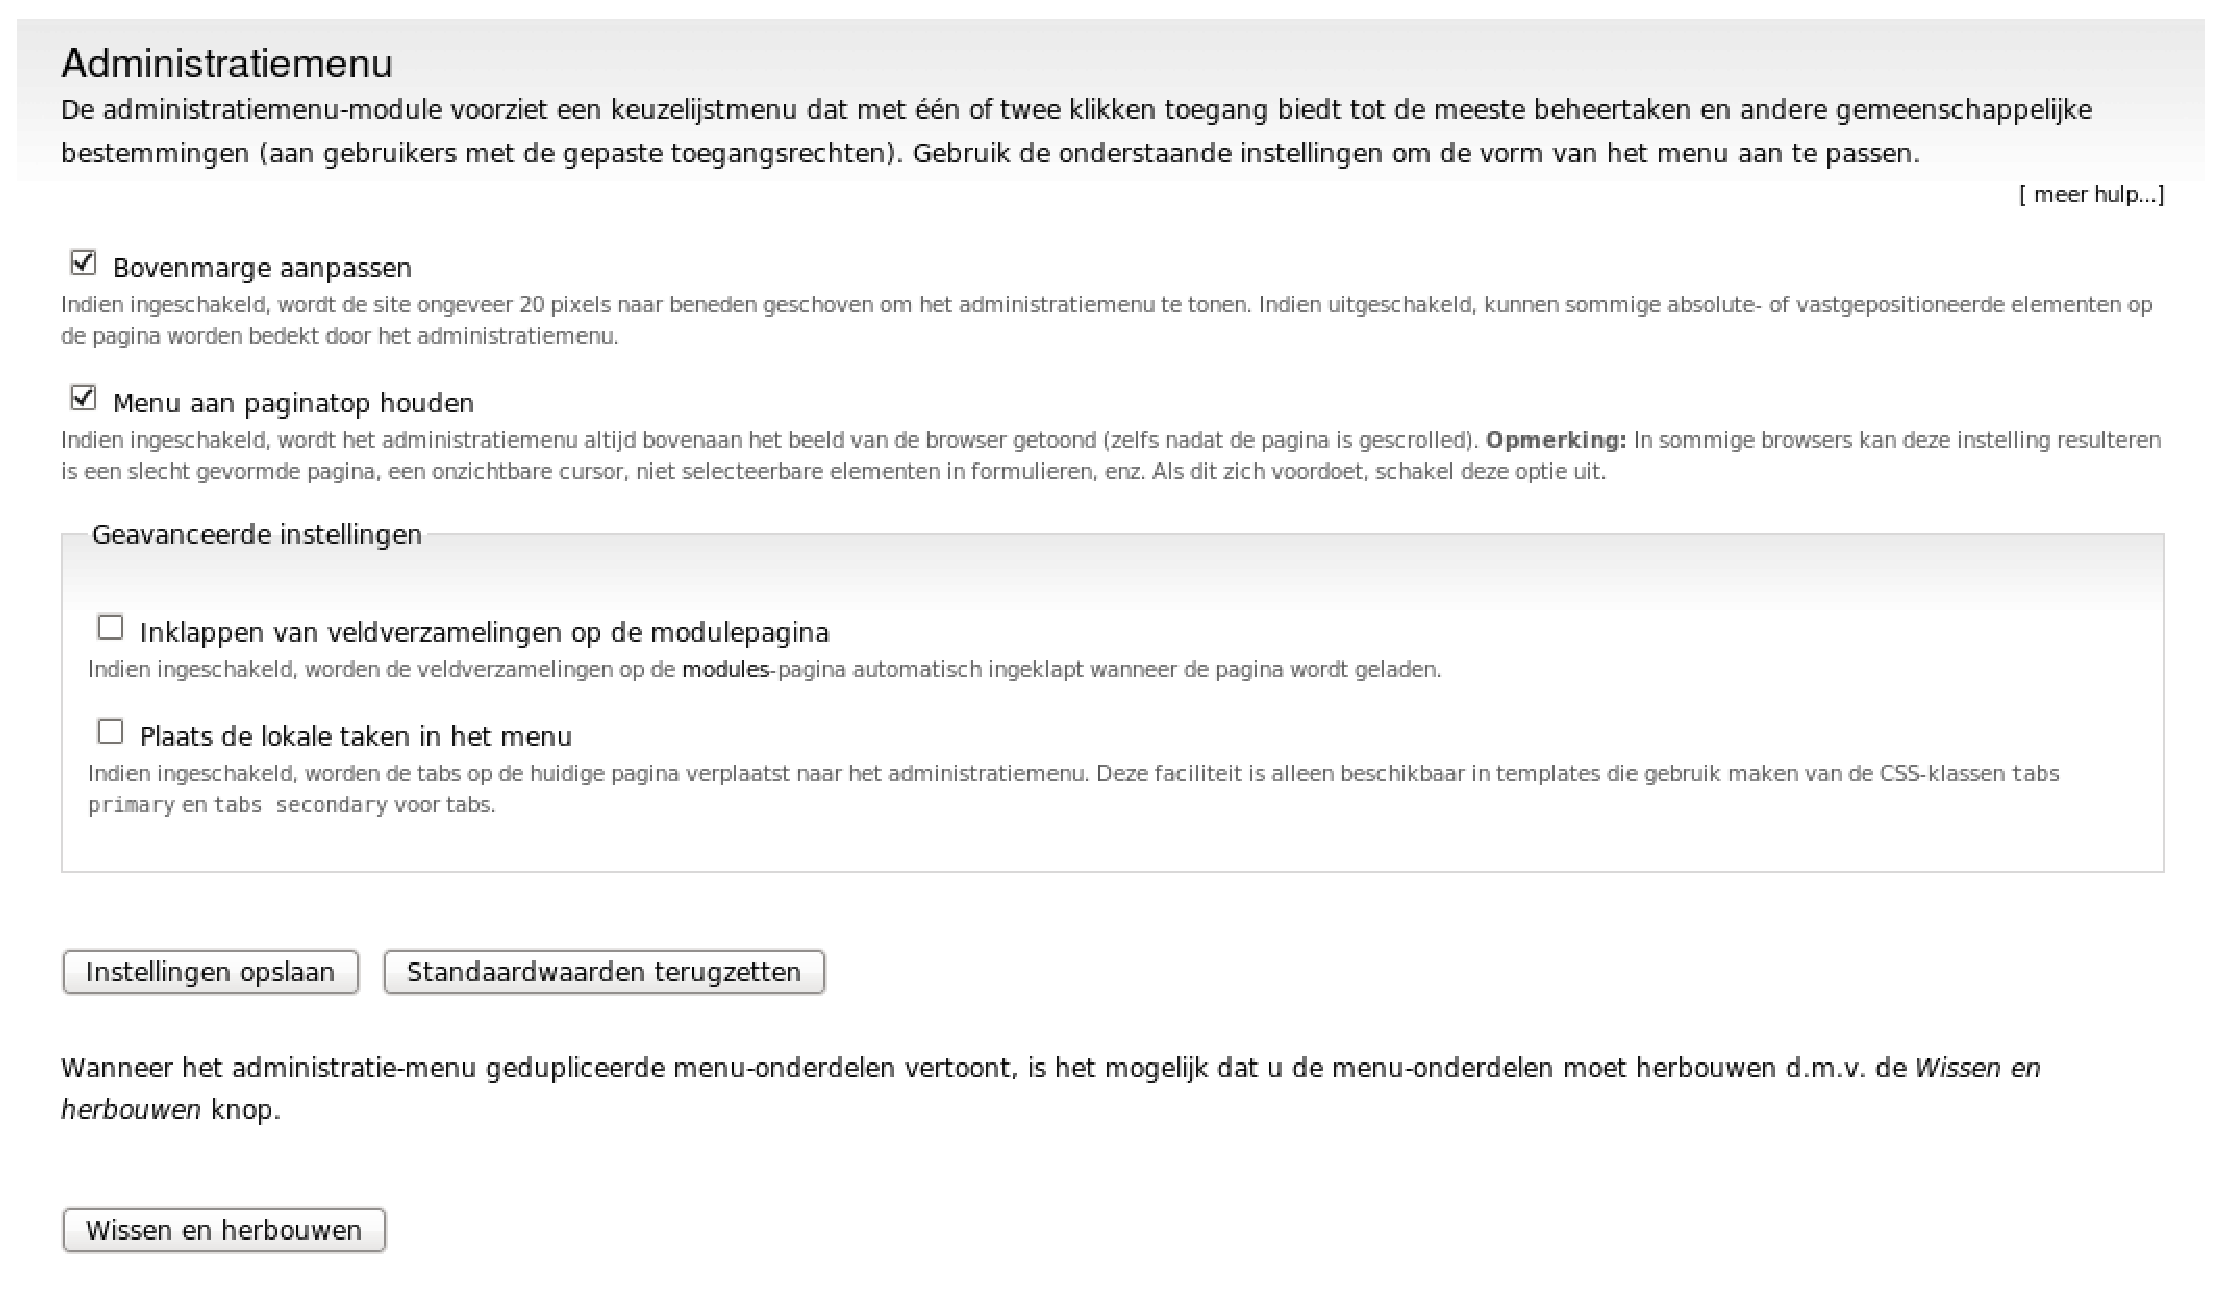
\includegraphics[scale=0.3,angle=0]{administratiemenu}
   \caption{administratiemenu.\label{white}}
 \end{figure}

\section{Beeldverwerkingstoolkit} \index{beeldverwerkingstoolkit}
Kies eventueel welke beeldverwerkingstoolkit gebruikt wordt als er meerdere
toolkits ge\"installeerd zijn. 
\begin{figure}[!h]
    \centering
   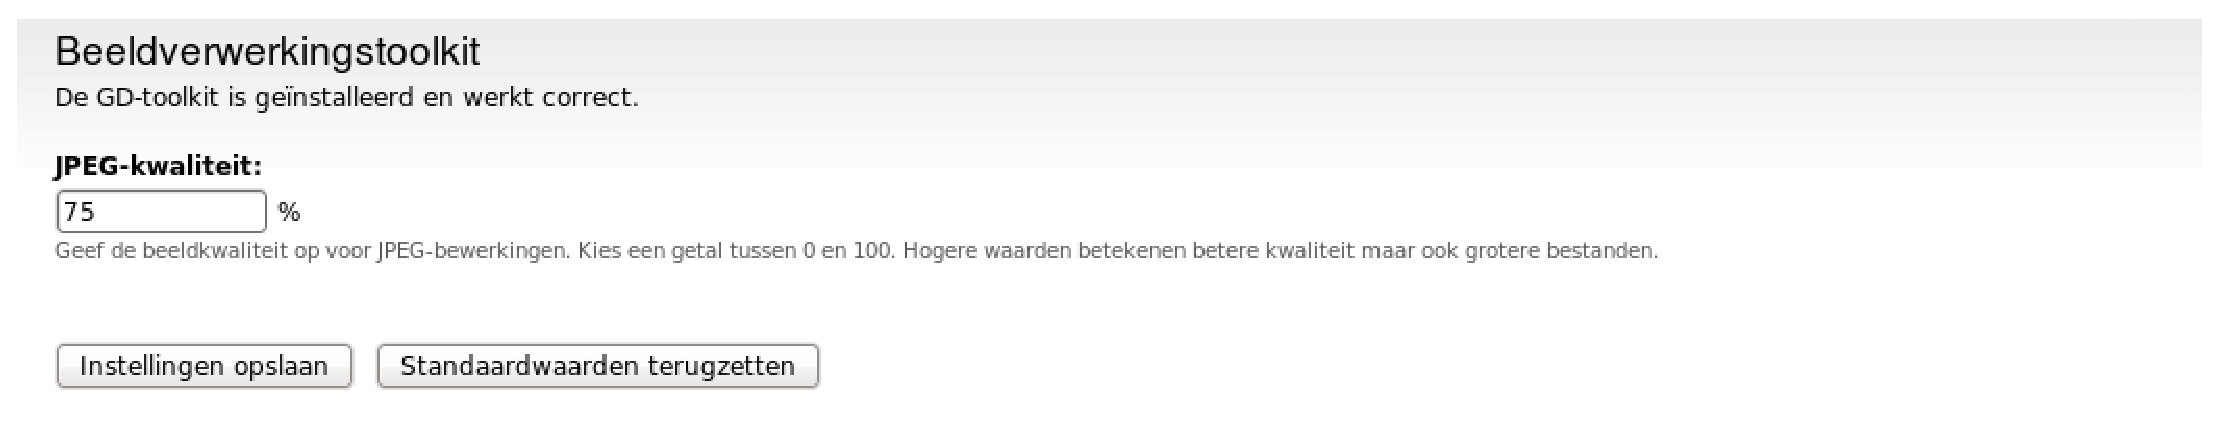
\includegraphics[scale=0.3,angle=0]{beeldverwerkingstoolkit}
   \caption{beeldverwerkingstoolkit.\label{white}}
 \end{figure}
 
\section{Beheertemplate} \index{beheertemplate}
Hier kan men de lay-out van de beheerinterface instellen. Bepaal met
 welke template de beheerpagina's worden weergegeven. Als u de
 'Systeemstandaard' kiest, worden de beheerpagina's met de zelfde template als
 de rest van de site weergegeven.
\begin{figure}[!h]
    \centering
   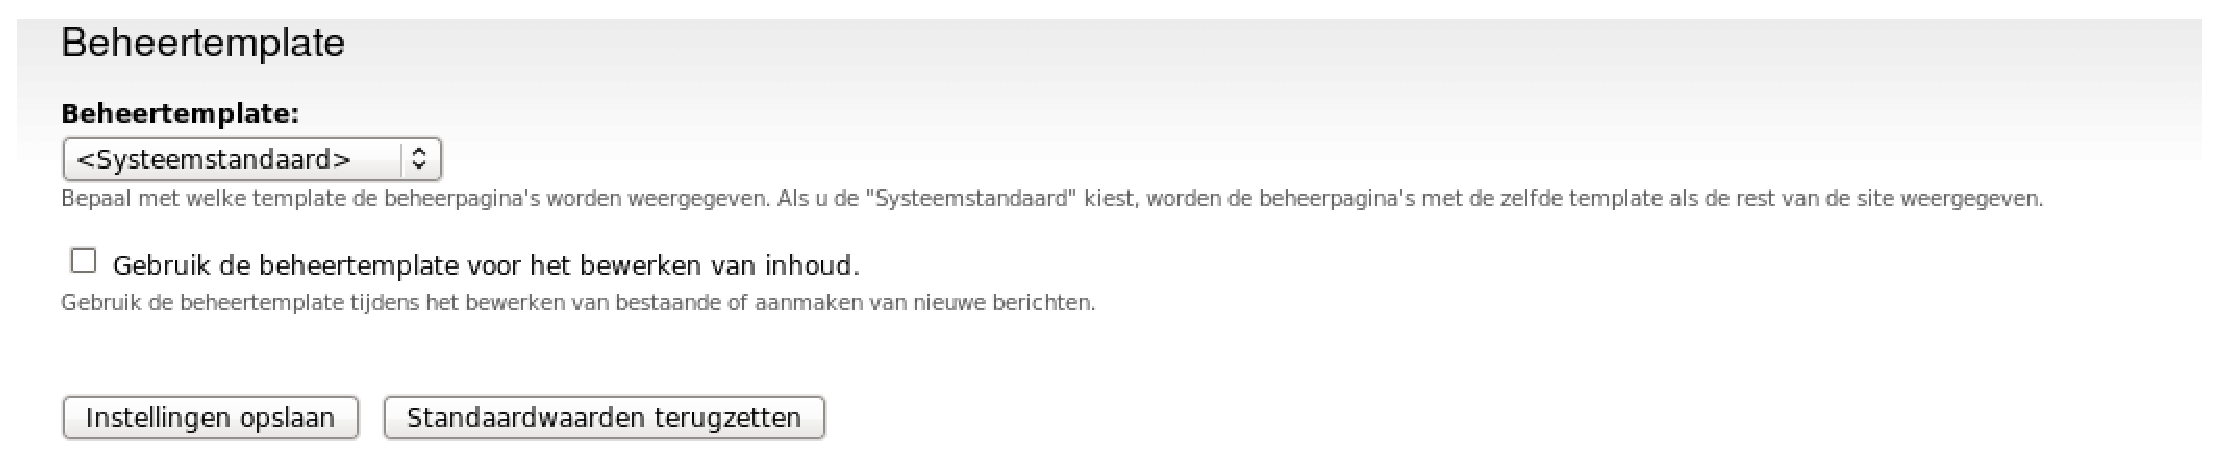
\includegraphics[scale=0.3,angle=0]{beheertemplate}
   \caption{beheertemplate.\label{white}}
 \end{figure} 
 
 
\section{Bestandssysteem} \index{bestandssysteem}
    Bepalen waar Drupal geuploade bestanden opslaat en hoe deze toegankelijk
    zijn. Een bestandssysteempad waar de bestanden zullen worden opgeslagen. De
    map moet bestaan en Drupal moet schrijftoegang hebben. Indien de downloadmethode publiek 
    is, dan moet deze map als relatief pad naar de Drupal-installatiemap worden opgegeven en 
    toegankelijk zijn via het internet. Indien de downloadmethode priv\'e is,
    dan mag de map niet te benaderen zijn via het internet. Indien u deze locatie wijzigt zullen alle downloadpaden wijzigen, 
    wat op een bestaande site onverwachte problemen kan opleveren.
 \begin{figure}[!h]
    \centering
   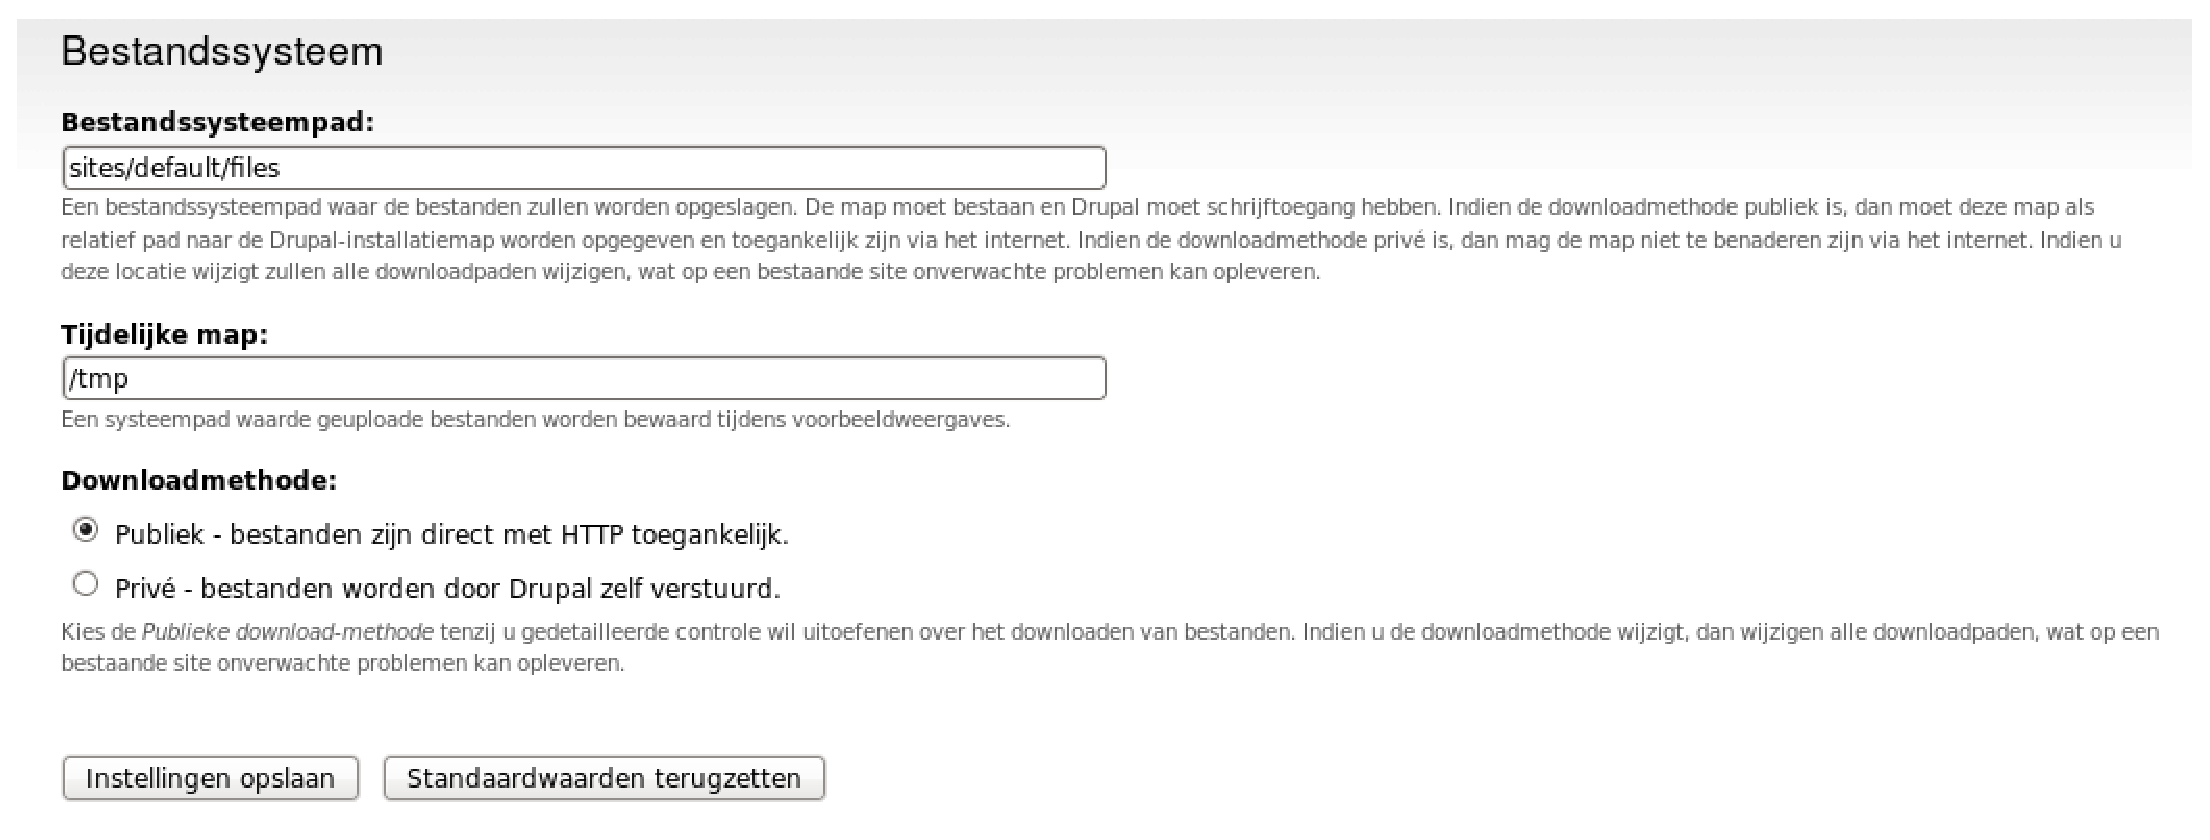
\includegraphics[scale=0.3,angle=0]{bestandssysteem}
   \caption{bestandssysteem.\label{white}}
 \end{figure}   
    
    
\section{Datum \index{datum} en tijd \index{tijd}} 
    Instellingen voor de weergave van datum en tijd en de standaard tijdzone van het Drupal systeem.
\begin{figure}[!h]
    \centering
   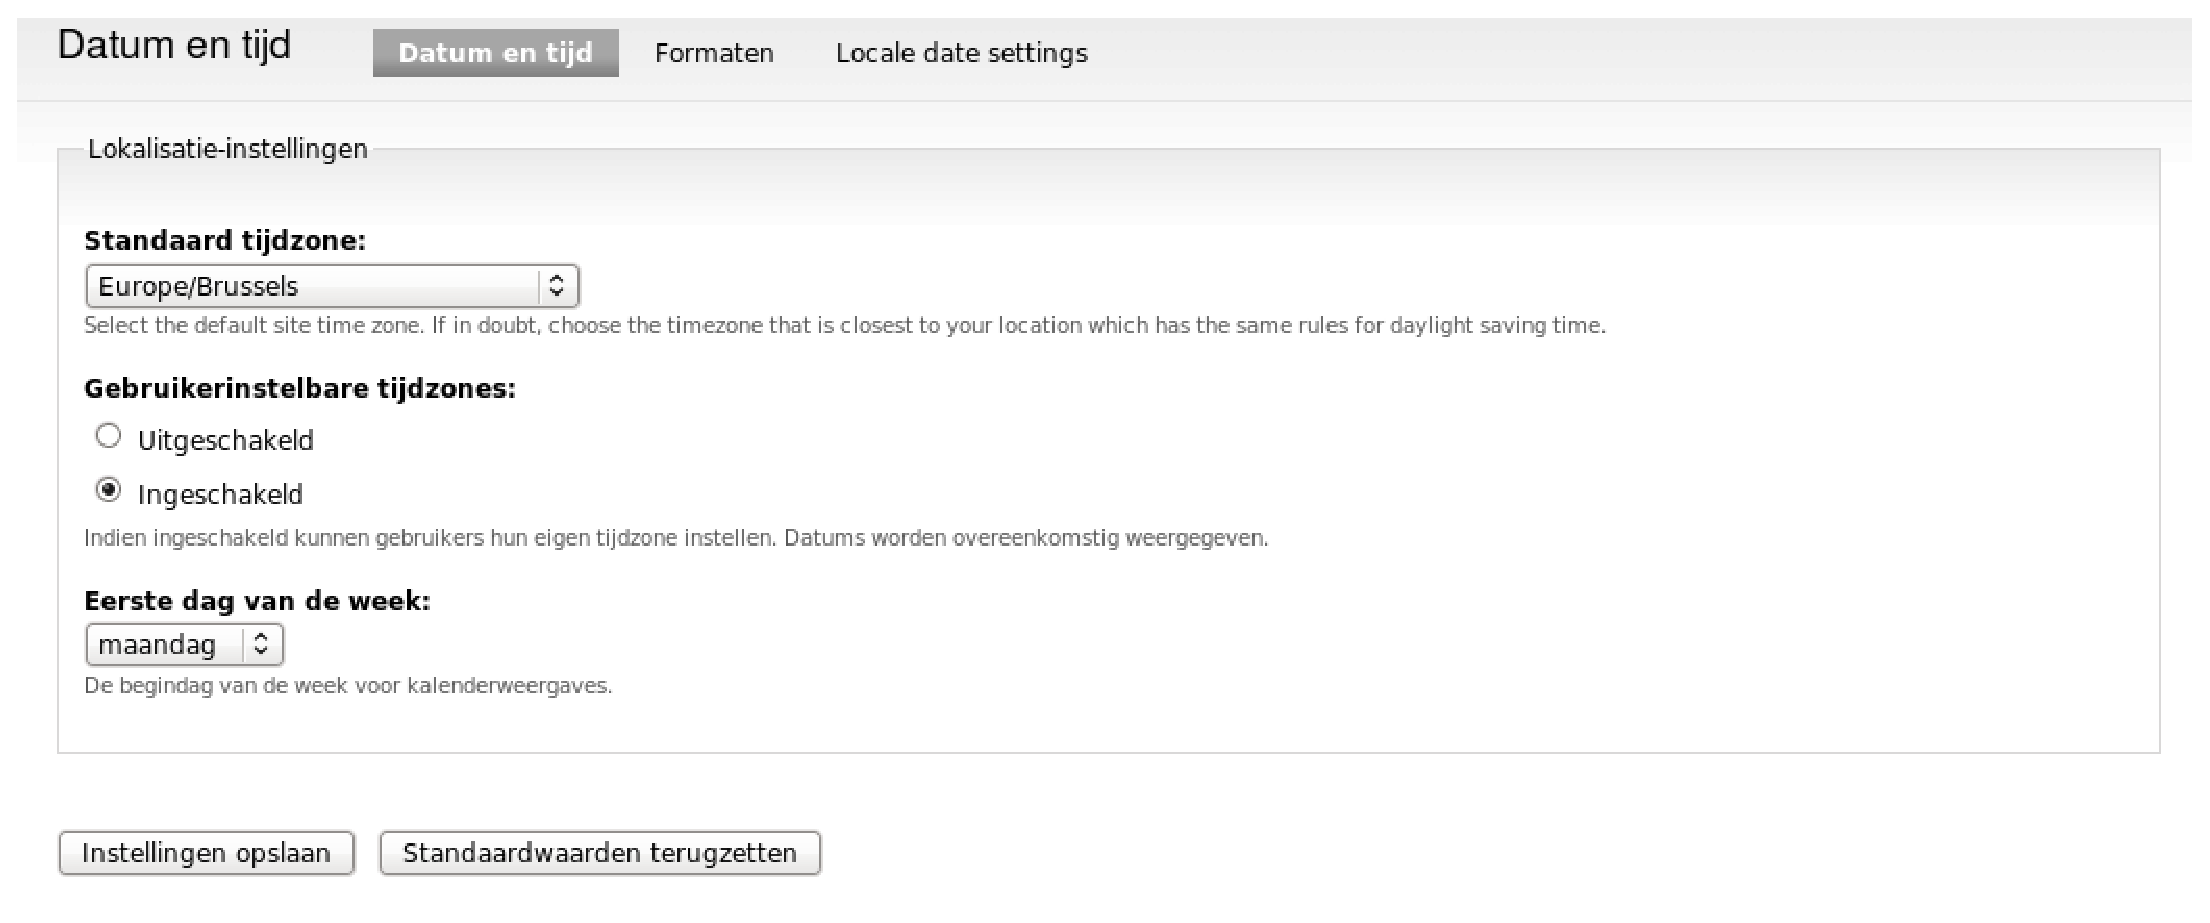
\includegraphics[scale=0.3,angle=0]{datum-tijd}
   \caption{datum-tijd.\label{white}}
 \end{figure}      
    
\section{Foutrapportage} \index{foutrapportage}
    Bepaal hoe Drupal omgaat met fouten, waaronder 403/404-fouten en PHP-foutrapportage.
 \begin{figure}[!h]
    \centering
   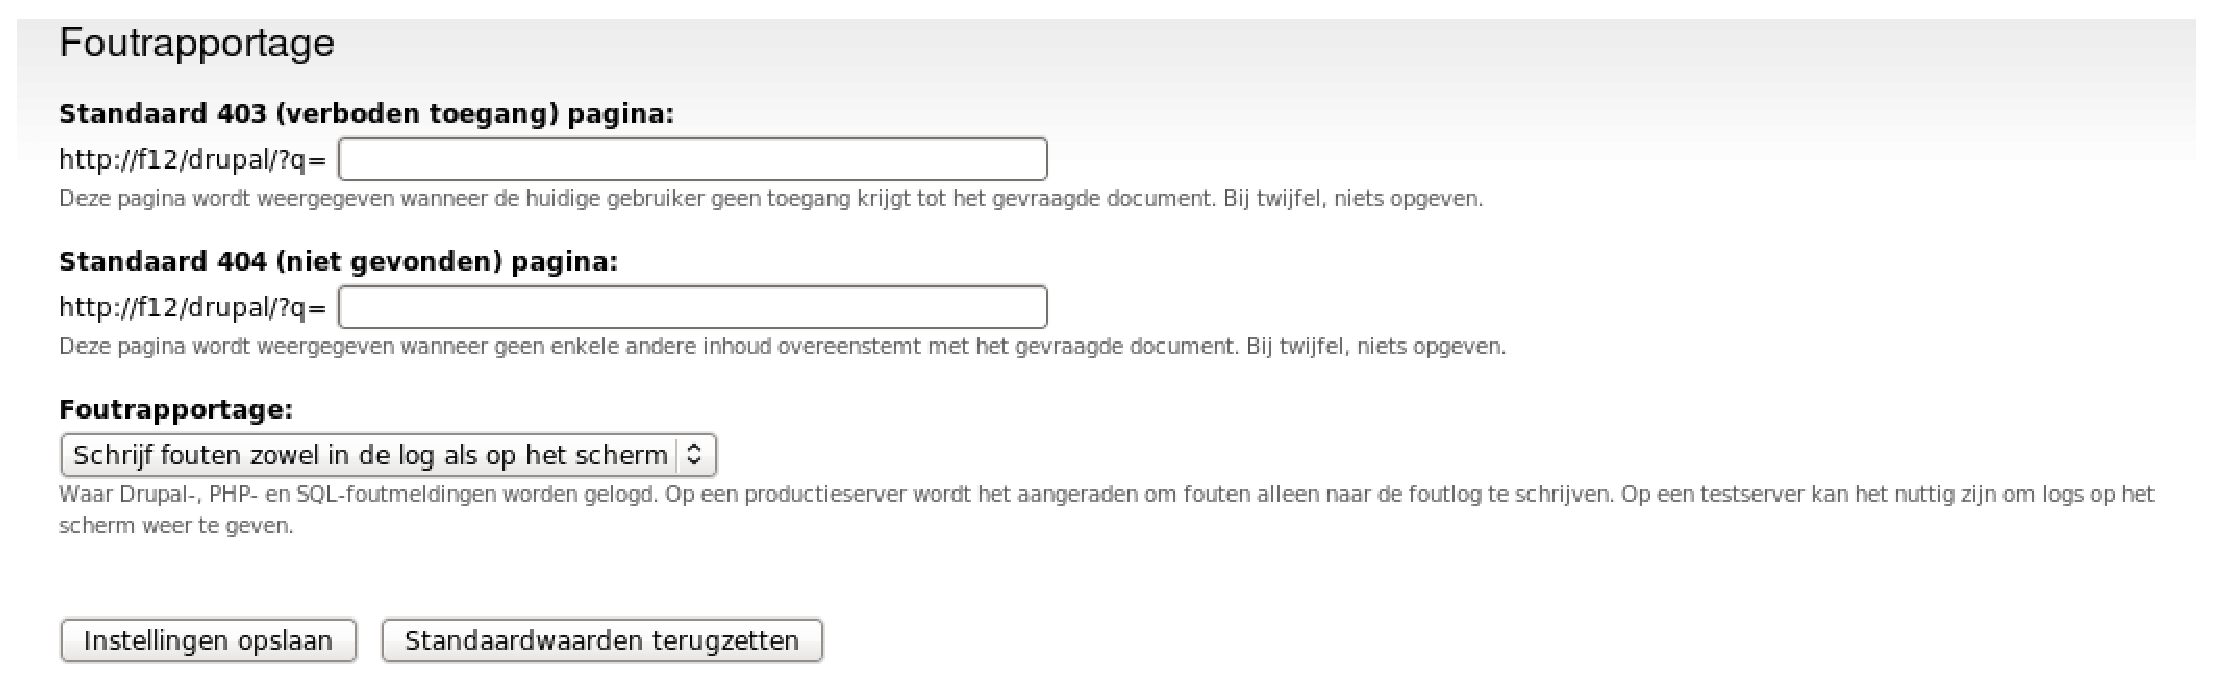
\includegraphics[scale=0.3,angle=0]{foutrapportage}
   \caption{foutrapportage.\label{white}}
 \end{figure}    
    
\section{Invoerformaten} \index{invoerformaten} 
    Bepaal hoe door gebruikers ingevoerde inhoud wordt gefilterd, inclusief toegestane HTML-tags. 
    Ondersteunt het inschakelen van filters die door modules worden aangeboden.
    \\
    Invoerformaten vormen het mechanisme waarmee Drupal de door gebruikers ingevoerde tekst verwerkt. 
    Ieder invoerformaat gebruikt filters om tekst te bewerken, de meeste invoerformaten passen meerdere 
    filters in een bepaalde volgorde toe. Ieder filter is voor een bepaald doel gebouwd en zal gewoonlijk 
    delen van de gebruikersinvoer verwijderen, omvormen of informatie toevoegen voordat deze wordt weergegeven. 
    Gebruikers kunnen tijdens het aanmaken of bewerken van inhoud tussen de beschikbare invoerformaten kiezen.
\\
Gebruik de onderstaande lijst om aan te geven welke invoerformaten voor welke rollen beschikbaar zijn en 
om het standaard invoerformaat te selecteren. Het standaardformaat is voor alle gebruikers beschikbaar. 
Voor gebruikers met toegangsrechten "filters beheren" zijn alle invoerformaten beschikbaar.
 \begin{figure}[!h]
    \centering
   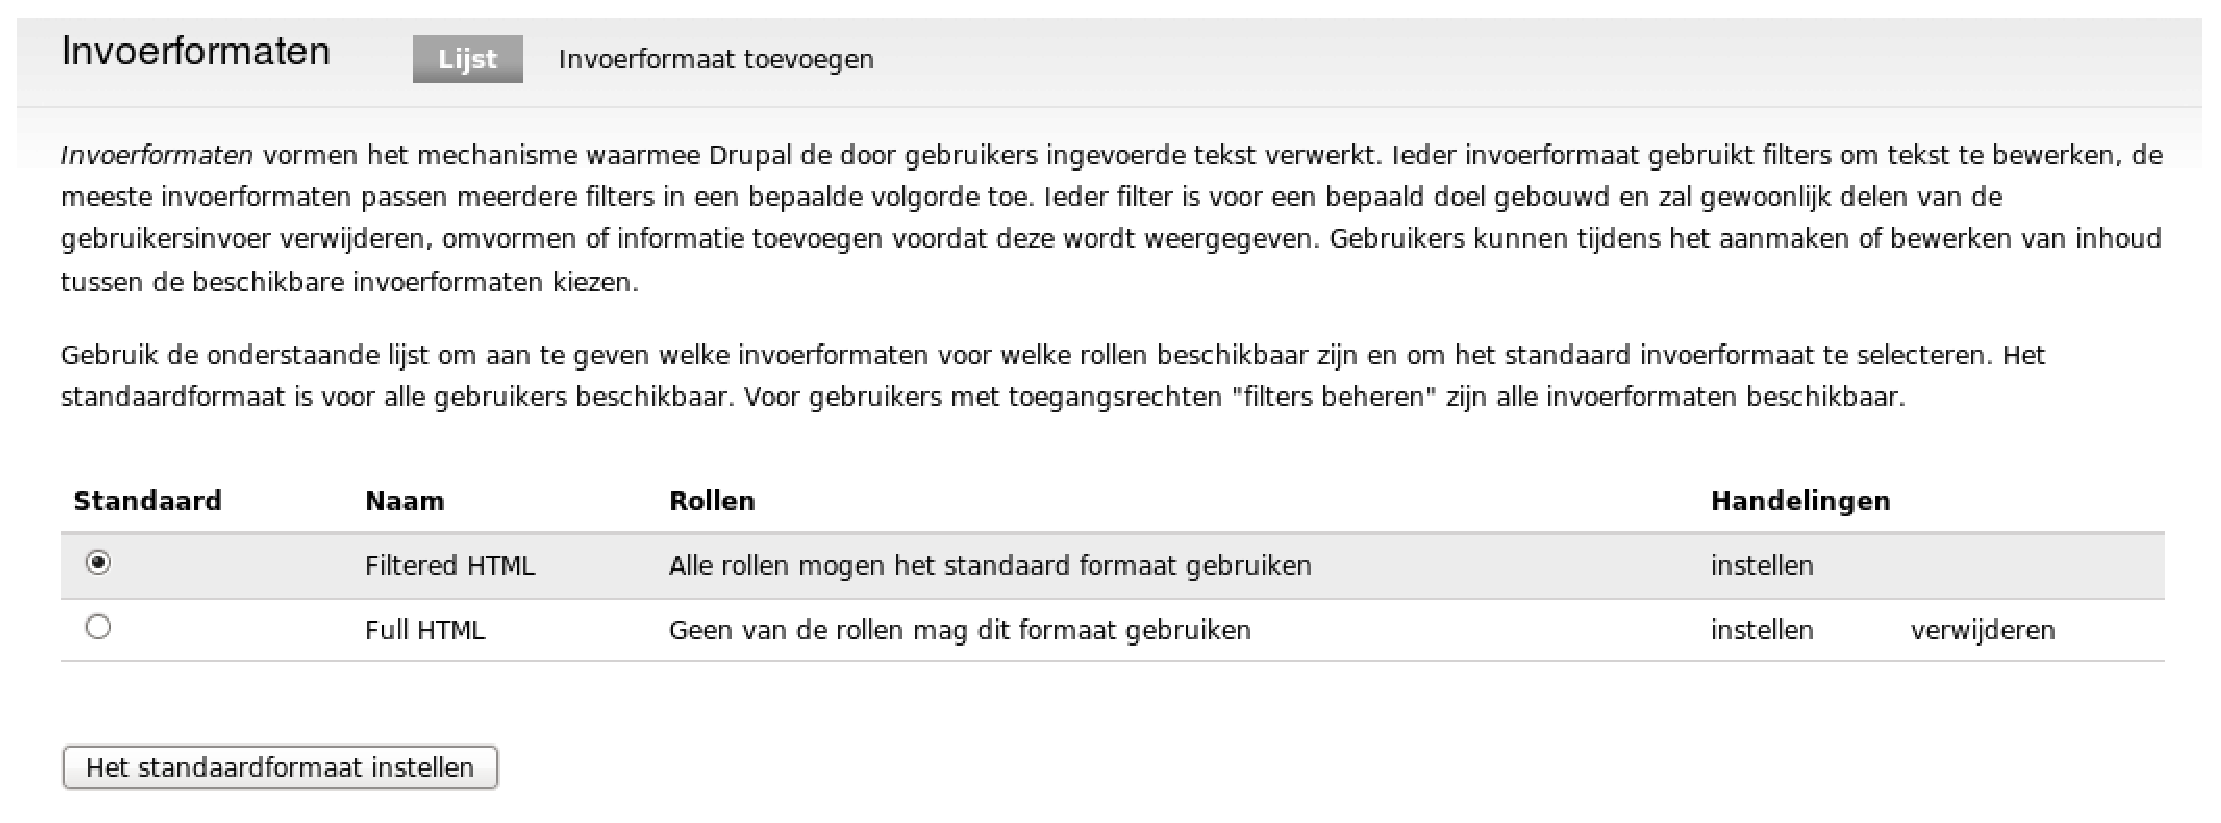
\includegraphics[scale=0.3,angle=0]{invoerformaten}
   \caption{invoerformaten.\label{white}}
 \end{figure}     
    
    
\section{Loggen \index{loggen} en waarschuwingen \index{waarschuwingen}} 
    Instellingen voor het logboek \index{logboek} en alarmmodules
    \index{alarmmodules}. Verschillende modules kunnen Drupals
    systeemgebeurtenissen doorsturen naar verschillende bestemmingen (het systeemlogboek, een database, e-mail, enz.). Dit is de meest gebruikelijke methode for kleine
    tot middelgrote sites op shared hosting. De logs kunnen op de beheerpagina's worden bekeken.
\begin{figure}[!h]
    \centering
   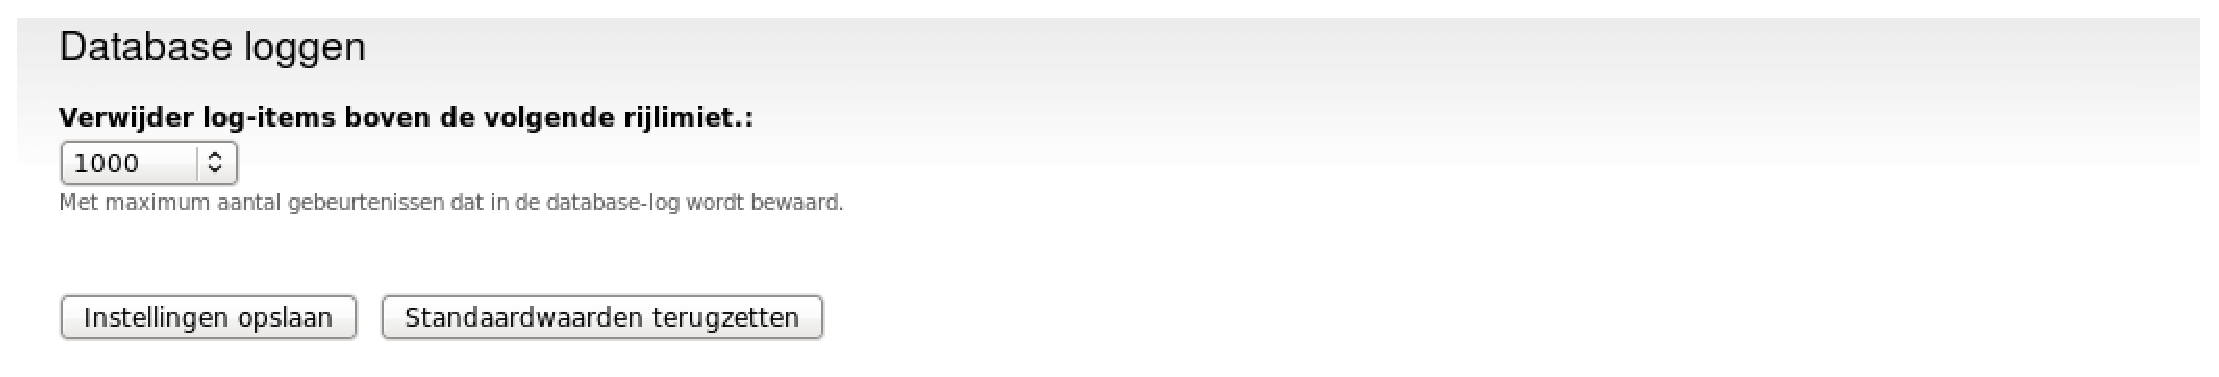
\includegraphics[scale=0.3,angle=0]{database-loggen}
   \caption{database-loggen.\label{white}}
 \end{figure}       
    
    
\section{Prestatie} \index{prestaties}
    Pagina-cache voor anonieme gebruikers in of uitschakelen en CSS- en JS-bandbreedte-optimalisatie instellingen.
\subsection{Pagina-cache} \index{pagina-cache} 
De pagina-cache inschakelen leidt tot significant betere prestaties. Drupal kan
  gecomprimeerde cache-pagina's bewaren en deze tonen aan anonieme gebruikers. Door een pagina op te slaan in de 
  cache hoeft Drupal deze pagina niet bij elk bezoek opnieuw op te bouwen.
\begin{figure}[!h]
    \centering
   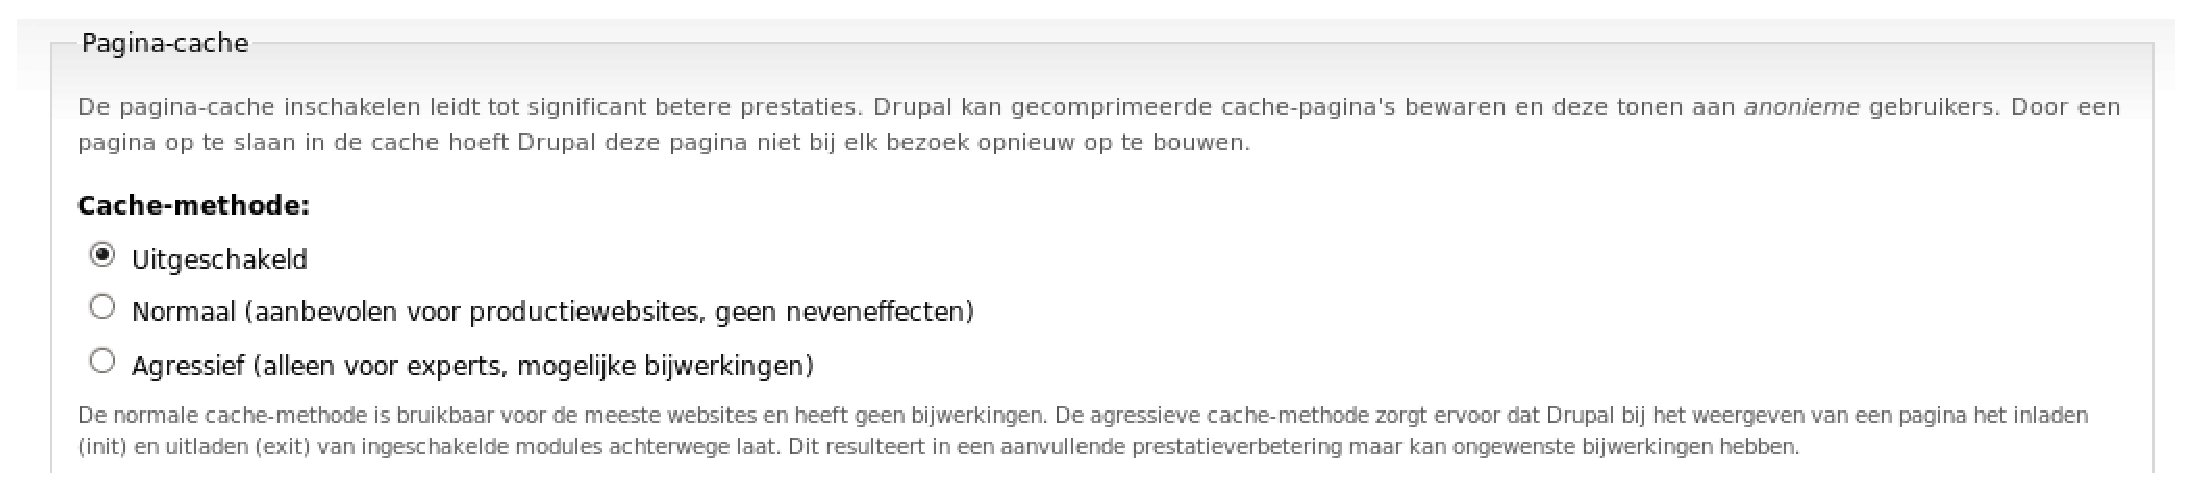
\includegraphics[scale=0.3,angle=0]{prestatie-pagina}
   \caption{prestatie-pagina.\label{white}}
 \end{figure} 
\subsection{Blok-cache} \index{blok-cache}
  Door de blok-cache in te schakelen kunnen gebruikers een prestatieverbetering
  merken; u voorkomt zo dat blokken bij elke raadpleging van een pagina opnieuw opgebouwd worden. 
  Indien de pagina-cache ook is ingeschakeld dan zal de blok-cache vooral geregistreerde gebruikers ten goede komen.
\begin{figure}[!h]
    \centering
   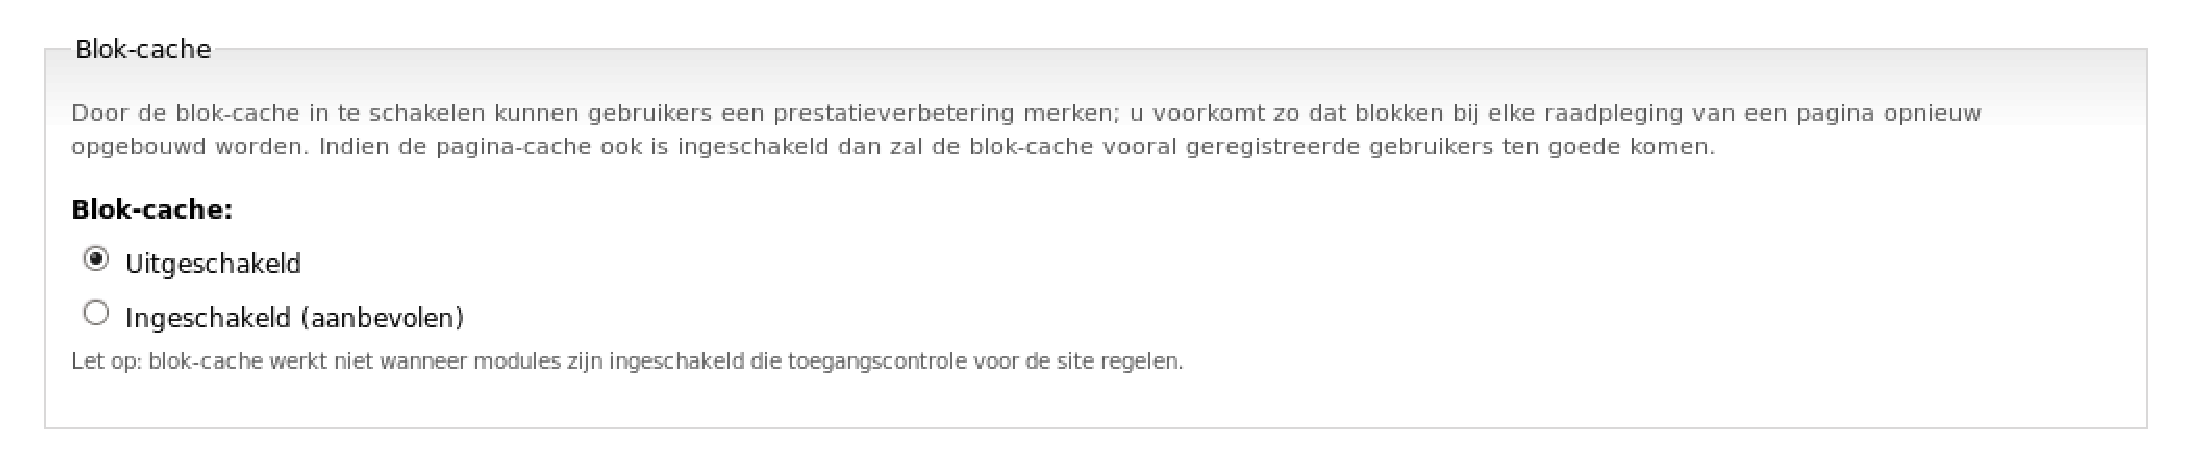
\includegraphics[scale=0.3,angle=0]{prestatie-blok}
   \caption{prestatie-blok.\label{white}}
 \end{figure}
\subsection{Bandbreedte-optimalisaties} \index{bandbreedte}
\index{optimalisaties} Drupal kan automatisch externe bronnen zoals CSS en JavaScript optimaliseren,
wat zowel de grootte als het aantal aanvragen aan uw website kan verminderen. CSS-bestanden kunnen samengevoegd 
en gecomprimeerd worden tot \'e\'en enkel bestand, terwijl JavaScript-bestanden
samengevoegd (maar niet gecomprimeerd) worden. Deze optimalisaties zijn optioneel en kunnen de serverbelasting, benodigde bandbreedte en paginalaadtijden verminderen.
\begin{figure}[!h]
    \centering
   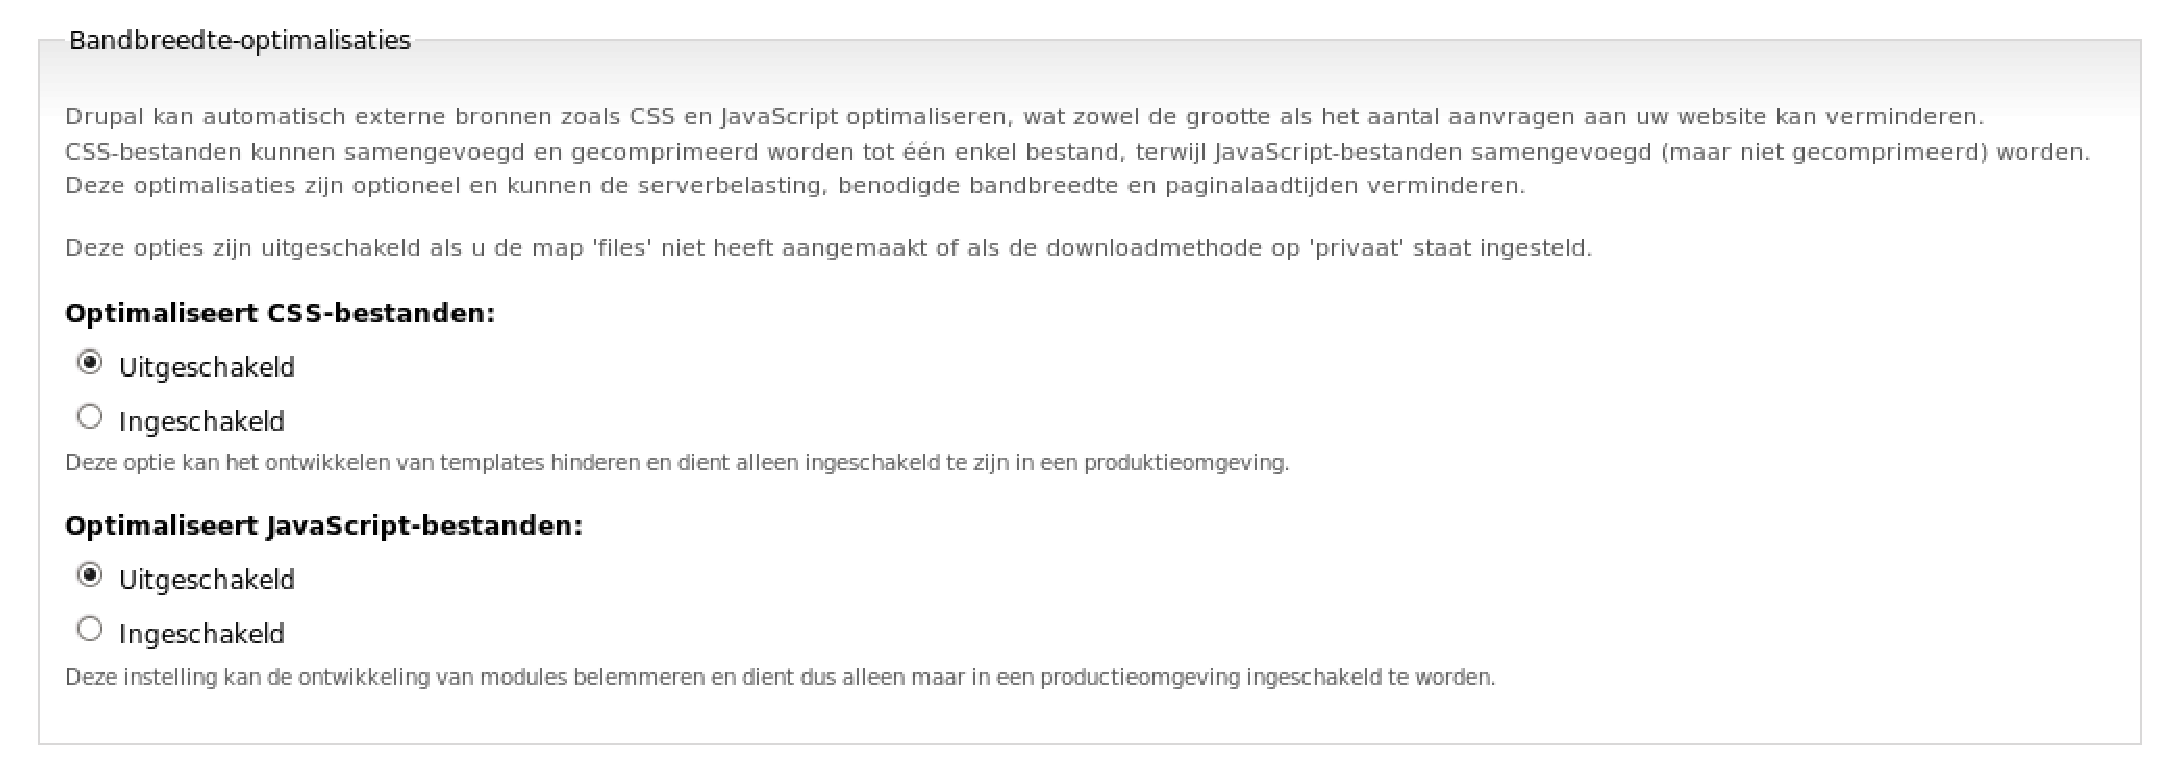
\includegraphics[scale=0.3,angle=0]{prestatie-bandbreedte}
   \caption{prestatie-bandbreedte.\label{white}}
 \end{figure}
\subsection{Cache-data opschonen} \index{cache-data}
Bufferen van gegevens verbetert de prestaties van de website, maar kan problemen
opleveren tijdens foutzoeken in nieuwe modules, templates of vertalingen als verouderde informatie wordt gebufferd. 
Klik op de onderstaande knop om alle gebufferde informatie op de site te verversen. Websites met veel dataverkeer zullen 
merkbaar langzamer reageren gedurende het opbouwen van de cache.
\begin{figure}[!h]
    \centering
   \includegraphics[scale=0.3,angle=0]{prestatie-cache}
   \caption{prestatie-cache.\label{white}}
 \end{figure}
 
\section{Schone URL's} \index{url}
    Schone URL's in- of uitschakelen. Deze optie zorgt ervoor dat Drupal
    'schone' URL's gebruikt (d.w.z. zonder ?q= in de URL.) 
\begin{figure}[!h]
    \centering
   \includegraphics[scale=0.3,angle=0]{schone-urls}
   \caption{schone-urls.\label{white}}
 \end{figure}

\section{Site-onderhoud} \index{onderhoud}
    Website offline brengen voor onderhoud of opnieuw online brengen. Als
    'Online' \index{online} is ingesteld, kunnen alle bezoekers uw site gewoon
    bezoeken. Als 'Offline' \index{offline} is ingesteld, kunnen alleen
    gebruikers met de 'Site-instellingen beheren' rechten uw site bezoeken om onderhoud te verrichten. Alle andere
    bezoekers zullen het off-line bericht zien dat u hieronder kunt instellen. 
    Geauthoriseerde gebruikers kunnen tijdens de 'Off-line' modus inloggen via
    de inlogpagina.
 \begin{figure}[!h]
    \centering
   \includegraphics[scale=0.3,angle=0]{site-onderhoud}
   \caption{site-onderhoud.\label{white}}
 \end{figure}   
    
\section{Talen} \index{talen}
    Instellingen voor de taal van inhoud en gebruikersinterface. \\
Wanneer meerdere talen zijn 
ingeschakeld, kan de tekst van de website-interface worden vertaald, kunnen geregistreerde 
gebruikers op de pagina Mijn account de taal van hun keuze instellen en kunnen auteurs de 
taal aangeven waarin de pagina-inhoud wordt ingediend. De standaardtaal wordt gebruikt voor 
anonieme gebruikers en voor gebruikers die geen voorkeurstaal hebben opgegeven.
\\
Voor iedere op de site beschikbare taal gebruikt u de link bewerken om de taal te configureren; 
waaronder naam van de taal, taalspecifiek pad of domein en de schrijfrichting van de 
taal (Links-naar-Rechts of Rechts-naar-Links). Deze talen zijn ook beschikbaar in de 
Taalkeuze bij het aanmaken van pagina's van inhoudstypen die meertaligheid ondersteunen.
\\
Gebruik de pagina Taal toevoegen om extra talen in te schakelen (en indien beschikbaar 
het vertaalpakket automatisch te importeren).\\ De pagina Vertalen om lokale
tekenreeksen te vertalen of de pagina Importeren om vertalingen uit losse .po-bestanden toe te voegen. 
Vertaalpakketten vindt u op de Drupal.org Translations-pagina.
\index{translation} \begin{figure}[!h]
    \centering
   \includegraphics[scale=0.3,angle=0]{talen}
   \caption{talen.\label{white}}
 \end{figure} 

\section{ Websitegegevens} \index{websitegegevens}
    Basis website gegevens instellen zoals naam van de site \index{naam},
    slogan \index{slogan}, e-mailadres, voorpagina \index{voorpagine}, enz.
    \begin{figure}[!h]
    \centering
   \includegraphics[scale=0.3,angle=0]{website-gegevens}
   \caption{website-gegevens.\label{white}}
 \end{figure}    
    
\section{Zoekinstellingen} \index{zoekinstellingen}
    Relevantie voor zoeken en andere indexeerinstellingen
    \index{indexeerinstellingen}. De Search-module \index{search-module} biedt
    de mogelijkheid om de inhoud van de site op trefwoord te doorzoeken. Zoeken is vaak de enige praktische manier om informatie op een grote site te vinden en kan voor het vinden van gebruikers en inhoud van de site worden toegepast.
\\
Om het zoeken op de website mogelijk te maken houdt de Drupal-zoekmachine een index bij 
van woorden die voorkomen in de inhoud van de site. Voor het opbouwen en bijhouden 
van deze index is cron nodig. Het indexeergedrag kan worden ingesteld op de pagina 
Zoekinstellingen. Op deze pagina kan het Aantal items dat per cron-uitvoering
wordt ge\"indexeerd worden ingesteld. Verminder dit aantal om timeout- en
geheugenfouten tijdens het indexeren te voorkomen.
  \begin{figure}[!h]
    \centering
   \includegraphics[scale=0.3,angle=0]{zoekinstellingen}
   \caption{zoekinstellingen.\label{white}}
 \end{figure}
blabla
%  \chapter{Gebruikersbeheer} \index{gebruikersbeheer}

\section{Gebruikers}
    Gebruikers opsommen, toevoegen en wijzigen.
 Met de User-module \index{user-module} kunnen gebruikers zichzelf registreren,
 inloggen en uitloggen. Gebruikers hebben voordeel van het registreren bij de site omdat informatie die 
 zij aan de site toevoegen verbonden is met hun account en omdat er aan hun rollen 
 toegangsrechten kunnen worden toegewezen. De User-module ondersteunt het samenstellen 
 van een fijnmazig stelsel van toegangsrechten waarmee de beheerder kan bepalen wat 
 een gebruiker wel en niet kan doen. Aan iedere gebruiker worden een of meerdere rollen 
 toegewezen. Standaard zijn twee rollen beschikbaar: anoniem: een gebruiker die niet is 
 ingelogd en geverifieerd: een ingelogde en geverifieerde gebruiker.
\\
Op de individuele accountpagina's kunnen gebruikers, al dan niet met hun eigen naam, 
hun persoonlijke instellingen wijzigen. Geregistreerde gebruikers moeten inloggen met 
hun lokale gebruikersnaam en een wachtwoord of optioneel met hun OpenID. OpenID is een 
veilige methode om op verschillende websites met \'e\'en wachtwoord en
gebruikersnaam in te loggen. In sommige configuraties kunnen geregistreerde gebruikers inloggen met hun 
gebruikersnaam en wachtwoord van een andere Drupal-website of met een site-specifieke methode inloggen.
\\
Wanneer een gebruiker toegang tot de website verkrijgt, ontvangt hij een uniek ID, 
het zogenaamde sessie-ID, dat in een cookie wordt opgeslagen. 
Om veiligheidsredenen bevat het cookie geen persoonlijke informatie maar fungeert 
het als de sleutel tot de persoonlijke informatie die op de server is opgeslagen. 
Gebruikers moeten het gebruik van cookies in hun browser hebben ingeschakeld om deze site te kunnen gebruiken.   
\begin{figure}[!h]
    \centering
   \includegraphics[scale=0.3,angle=0]{gebruikers}
   \caption{gebruikers.\label{white}}
 \end{figure}    
    
\section{Gebruikersinstellingen} \index{gebruikersinstellingen}
    Standaard gedrag voor gebruikers bepalen, waaronder registratievereisten, e-mail en gebruikersafbeeldingen.
\subsection{Instellingen gebruikersregistratie}  \index{gebruikersregistratie}
\begin{figure}[!h]
    \centering
   \includegraphics[scale=0.3,angle=0]{publieke-registraties}
   \caption{publieke-registraties.\label{white}}
 \end{figure} 
\subsection{Gebruikersinstellingen e-mail} \index{e-mail}
Drupal stuurt e-mails wanneer een nieuwe gebruiker zich registreert op uw site,
 en optioneel, kan ook gebruikers informeren over andere account-wijzigingen. 
 Gebruikmakend van eenvoudige sjablonen, kunnen informerende e-mails 
 ingesteld worden om te voldoen aan specifieke behoefte van uw site. 
 \begin{figure}[!h]
    \centering
   \includegraphics[scale=0.3,angle=0]{gebruikersinstellingen-email}
   \caption{gebruikersinstellingen-email.\label{white}}
 \end{figure} 
    
    
\section{Rollen} \index{rollen}
    Rollen opsommen, toevoegen en wijzigen.
Met rollen kunt u de beveiliging en het beheer van Drupal nauwkeurig bepalen.
 Een rol omvat een groep gebruikers die rechten hebben zoals vastgelegd in toegangsrechten . 
 Voorbeelden van rollen zijn: anonieme gebruiker, geverifieerde gebruiker, moderator, beheerder etc. 
 U kunt zelf de namen van de verschillende rollen bepalen. Met bewerken kunt u een rol verwijderen. 
 Drupal heeft standaard twee rollen:
 \begin{itemize}
\item Anonieme gebruiker: deze rol wordt gebruikt voor gebruikers die geen
account hebben of niet geverifieerd zijn.
\item Geverifieerde gebruiker: deze rol wordt automatisch toegekend aan alle
gebruikers die zijn ingelogd.
\end{itemize}
\begin{figure}[!h]
    \centering
   \includegraphics[scale=0.3,angle=0]{rollen}
   \caption{rollen.\label{white}}
 \end{figure} 
 
    
\section{Toegangsrechten} \index{toegangsrechten}
Met toegangsrechten kunt u bepalen wat gebruikers op de site kunnen doen. Iedere
gebruikersrol (gedefinieerd op de pagina rollen) heeft een eigen set toegangsrechten. 
Zo kunt u bijvoorbeeld gebruikers met de rol 'Beheerder' rechten geven voor
'nodes beheren' maar deze mogelijkheid aan gewone 'geverifieerde' gebruikers
onthouden. U kunt de toegangsrechten gebruiken om bepaalde functionaliteit 
beschikbaar te maken voor groepen gebruikers (bijvoorbeeld voor ingelogde gebruikers). 
Met toegangsrechten kan ook de last van het beheren van een drukke site over 
verschillende betrouwbare gebruikers worden verdeeld.
\begin{figure}[!h]
    \centering
   \includegraphics[scale=0.3,angle=0]{toegangsrechten}
   \caption{toegangsrechten.\label{white}}
 \end{figure}


\section{Toegangsregels} 
    Toegangsregels opsommen en aanmaken om gebruikers te weren op basis van gebruikersnaam, e-mailadres en IP-adres.
De toegang op basis van gebruikersnaam en e-mailadres vaststellen voor nieuwe en
bestaande accounts \index{accounts} (account die op dit moment zijn ingelogd
worden niet uitgelogd). Wanneer een gebruikersnaam of e-mailadres overeenkomt met een weigeren-regel en niet met een toestaan-regel, dan zal deze account niet 
mogen inloggen of aangemaakt worden. Een host-regel is werkzaam voor iedere pagina, niet alleen de inlog-pagina.
\begin{figure}[!h]
    \centering
   \includegraphics[scale=0.3,angle=0]{toegangsregels}
   \caption{toegangsregels.\label{white}}
 \end{figure}
blabla
%  \chapter{Rapporten}

\section{Recente logs} \index{logs}
    Gebeurtenissen bekijken die recent zijn gelogd.
De DBlog-module \index{dblog-module} bewaakt de website en slaat
systeemgebeurtenissen op in een logboek dat iedere gebruiker met toestemming op een later tijdstip kan bekijken. 
Het logboek \index{logboek} is een eenvoudige lijst van geregistreerde
gebeurtenissen zoals gebruiks- en prestatiegegevens, fouten, waarschuwingen en operationele informatie. 
Aangezien het logboek vaak de enige bron van informatie is, is het belangrijk dat dit 
regelmatig gecontroleerd wordt.
 \begin{figure}[!h]
    \centering
   \includegraphics[scale=0.4,angle=0]{recente-logs1}
   \caption{recente-logs1.\label{white}}
 %  \small \\Drupal
 \end{figure}
    
\subsection{Database logging}
De DBlog-module bewaakt de website en slaat systeemgebeurtenissen op in een logboek dat iedere gebruiker
 met toestemming op een later tijdstip kan bekijken. Dit is nuttig voor sitebeheerders die een snel overzicht
willen van activiteiten op de site. Het logboek slaat ook de volgorde van de gebeurtenissen op, 
wat nuttig kan zijn om fouten op de site op te lossen.
\\
Het dblog-logboek is een eenvoudige lijst van geregistreerde gebeurtenissen zoals gebruiks- en prestatiegegevens, 
fouten, waarschuwingen en operationele informatie. Beheerders zouden regelmatig de dblog moeten controleren om er 
zeker van te zijn dat de site goed functioneert.
\\\\
opm: Lees voor meer informatie het online-handboek over de Dblog-module.
 \begin{figure}[!h]
    \centering
   \includegraphics[scale=0.4,angle=0]{recente-logs2}
   \caption{recente-logs2.\label{white}}
 %  \small \\Drupal
 \end{figure}
\subsection{Database logging beheerpagina's}
\begin{itemize}
 \item Database loggen
 \item Meest voorkomende fouten 'Geen toegang'
 \item Meest voorkomende fouten 'pagina niet gevonden'
 \item Recente logs
\end{itemize}

\section{Meest populaire zoekwoorden} \index{zoekwoorden}
    Bekijk de meest populaire zoekwoorden
\begin{figure}[!h]
    \centering
   \includegraphics[scale=0.4,angle=0]{populaire-zoekwoorden}
   \caption{populaire-zoekwoorden.\label{white}}
 %  \small \\Drupal
 \end{figure}    
    
    
\section{Meest voorkomende fouten 'Geen toegang'\index{fout - geen toegang}} 
    'Geen toegang' fouten (403) bekijken.
\begin{figure}[!h]
    \centering
   \includegraphics[scale=0.4,angle=0]{geen-toegang}
   \caption{geen-toegang.\label{white}}
 %  \small \\Drupal
 \end{figure}     
    
    
\section{Meest voorkomende fouten 'pagina niet gevonden'\index{fout - niet
gevonden}}  'Pagina niet gevonden' fouten (404) bekijken.
\begin{figure}[!h]
    \centering
   \includegraphics[scale=0.4,angle=0]{pagina-niet-gevonden}
   \caption{pagina-niet-gevonden.\label{white}}
 %  \small \\Drupal
 \end{figure} 



\section{Beschikbare updates} \index{updates}
    Ontvang een statusrapport van beschikbare nieuwe versies voor
 ge\"installeerde modules en templates.
\\
Hier vindt u meer informatie over beschikbare nieuwe versies voor de
ge\"installeerde modules en templates. Let op, iedere module of template is een
onderdeel van een 'project' dat dezelfde of een andere naam kan hebben en meerdere modules of templates kan omvatten.\\
Een groot aantal uitbreidingsmodules en uitbreidingstemplates zijn beschikbaar om de functionaliteit van 
uw website uit te breiden of de layout te wijzingen.\\
Laatste controle: 1 sec geleden (Handmatig controleren)\\
Er is geen informatie beschikbaar over potenti\"ele updates voor de
ge\"installeerde modules en templates. Om op nieuwe versies te controleren
kunt u cron instellen of kunt u handmatig controleren. Even geduld, het controleren op nieuwe versies kan enige tijd duren.
\begin{figure}[!h]
    \centering
   \includegraphics[scale=0.4,angle=0]{updates}
   \caption{updates.\label{white}}
 %  \small \\Drupal
 \end{figure}
 
\section{Status rapportage} \index{rapportage}
Weergave van de systeemstatus en eventueel gedetecteerde problemen.\\\\
Hier vindt u een kort overzicht van de parameters van uw site en eventuele
problemen met uw installatie. Het kan nuttig zijn deze informatie mee te geven bij het indienen van ondersteuningsvragen op de forums van drupal.org en in de project 'issue queues'.
 \begin{figure}[!h]
    \centering
   \includegraphics[scale=0.4,angle=0]{status_rapportage}
   \caption{Status rapportage.\label{white}}
 %  \small \\Drupal
 \end{figure}


\part{Inhoud aanmaken}
% \chapter{Standaard inhoudtypen} \index{inhoudstypen}
\section{Inhoud aanmaken}
Bij de aanmaak van een nieuwe node moet eerst een inhoudstype worden gekozen.
Hiermee worden de basiskenmerken van de node vastgelegd.

Drupal kent standaard drie verschillende inhoudstypes. De namen van de eerste
twee types worden niet vertaald bij het invoeren van de vertaling van de website.
\begin{itemize}
\item Pagina
\item Verhaal
\item Boek (indien de boekmodule ingeschakeld is).
\end{itemize}

\subsection{pagina} \index{pagina} \index{page}
Bedoeld voor een statische pagina \footnote{In de vertaalde website staat
'page'}, zoals een contactpagina of een 'over ons' pagina.

\subsection{verhaal} \index{verhaal} \index{story}
Verhalen \footnote{In de vertaalde website staat 'story'} zijn de meest simpele
artikelen: ze hebben een titel, een voorproefje en een berichttekst. Andere modules 
kunnen meer eigenschappen toevoegen. Het voorproefje is een integraal onderdeel van de 
berichttekst. Verhalen kunnen gebruikt worden voor een persoonlijke blog, voor nieuwsartikelen of een kort bericht.
De standaardinstelling is dat een verhaal op de voorpagina wordt gepubliceerd.

\subsection{Boek} \index{boek}

Een boek \footnote{In de vertaalde website staat 'book page'} is een
gezamenlijke schrijfinspanning: gebruikers kunnen samen de pagina's van het boek
schrijven, de pagina's in de juiste volgorde plaatsen en eerder geschreven
pagina's nalezen en verbeteren. Wanneer u informatie wilt delen, of een pagina van een boek leest die u niet bevalt, of denkt dat u een 
bepaalde pagina beter kunt schrijven, kunt u er zelf iets aan doen.
\\
Boekpagina's zijn automatisch voorzien van links naar aangrenzende pagina's en hebben daarmee een eenvoudig navigatiesysteem.


\section{Inhoudtypen}
Als voorbeeld gebruik ik het 'boekpagina' type.
 \begin{figure}[!h]
    \centering
   \includegraphics[scale=0.3,angle=0]{book_page_aanmaken}
   \caption{Boek pagina aanmaken.\label{white}}
 \end{figure}

\subsection{Menu-instellingen} \index{menu-instellingen}
De kenmerken van ieder inhoudstype is simpel aan te passen.
 \begin{figure}[!h]
    \centering
   \includegraphics[scale=0.3,angle=0]{menu-instellingen}
   \caption{Menu-instellingen.\label{white}}
 \end{figure}
\begin{itemize}
  \item  Titel van menulink: \index{menulink} De tekst van de link
  \index{link} naar dit item, die moet verschijnen in het menu. Leeglaten als u
  voor deze pagina geen menu-item wilt toevoegen.
  \item  Bovenliggend onderdeel: Het maximum aantal sub-onderdelen dat onder een
  menu-onderdeel geplaatst kan worden is 9. Sommige menu-onderdelen kunnen niet als bovenliggend 
  onderdeel geselecteerd worden omdat dan het aantal sub-onderdelen deze 9 overschrijdt.
  \begin{figure}[!h]
    \centering
   \includegraphics[scale=0.3,angle=0]{bovenliggend-onderdeel}
   \caption{bovenliggend-onderdeel.\label{white}}
 \end{figure}
  \item  Gewicht: Optioneel. In het menu zullen zwaardere onderdelen naar de
  bodem zakken en lichtere onderdelen hoger worden gepositioneerd.
\end{itemize}

\subsection{Invoerformaat} \index{invoerformaat}

 \begin{figure}[!h]
    \centering
   \includegraphics[scale=0.3,angle=0]{invoerformaat}
   \caption{Invoerformaat.\label{white}}
 \end{figure}
Filtered HTML \index{filtered html} \index{html}
        \begin{itemize}
            \item Adressen van webpagina's en e-mailadressen worden automatisch naar links omgezet.
            \item Toegelaten HTML-tags: $<$a$>$ $<$em$>$ $<$strong$>$ $<$cite$>$
            $<$code$>$ $<$ul$>$ $<$ol$>$ $<$li$>$ $<$dl$>$ $<$dt$>$ $<$dd$>$
            \item Regels en paragrafen worden automatisch gesplitst.
        \end{itemize} 
Full HTML \index{full-html}
        \begin{itemize}
            \item Adressen van webpagina's en e-mailadressen worden automatisch
            naar links omgezet.
            \item Regels en paragrafen worden automatisch gesplitst.
        \end{itemize}

\subsection{Boekstructuur} \index{boekstructuur}
 \begin{figure}[!h]
    \centering
   \includegraphics[scale=0.3,angle=0]{boekstructuur}
   \caption{Boekstructuur.\label{white}}
 \end{figure}
\begin{itemize}
  \item Book: De pagina zal deel uitmaken van het geselecteerde boek.
  \item Gewicht: \index{gewicht} Pagina's op een bepaald niveau worden eerst
  naar gewicht en dan naar titel gerangschikt.
\end{itemize}

\subsection{Revisie-informatie} \index{revisie-informatie}
 \begin{figure}[!h]
    \centering
   \includegraphics[scale=0.3,angle=0]{revisie-informatie}
   \caption{Revisie-informatie.\label{white}}
 \end{figure}
Hier kan je een nieuw revisie aanmaken. In het logbericht geef je uitleg
bij de toevoegingen of aanpassingen, die andere auteurs helpen uw beweegredenen te begrijpen.

\subsection{URL-pad-instellingen} \index{url-pad}
 \begin{figure}[!h]
    \centering
   \includegraphics[scale=0.3,angle=0]{url-pad-instellingen}
   \caption{URL-pad-instellingen.\label{white}}
 \end{figure}
Specificeer optioneel een alternatief pad waarop deze data kan worden bereikt.
Gebruik bijvoorbeeld ''over ons'' als een pagina over de organisatie wordt
geschreven. Gebruik een relatief pad en zet geen slash achter de alias, anders zal deze niet werken.

\subsection{Reactie-instellingen} \index{reactie-instellingen}
Hier dient U een titel op te geven, dit is een verplicht veld.
 \begin{figure}[!h]
    \centering
   \includegraphics[scale=0.3,angle=0]{reactie-instellingen}
   \caption{Reactie-instellingen.\label{white}}
 \end{figure}
\begin{itemize}
  \item Uitgeschakeld
  \item Alleen lezen
  \item Lezen/Schrijven
\end{itemize}

\subsection{Auteursinformatie} \index{auteursinformatie}
Hier dient U een titel op te geven, dit is een verplicht veld.
 \begin{figure}[!h]
    \centering
   \includegraphics[scale=0.3,angle=0]{auteursinformatie}
   \caption{Auteursinformatie.\label{white}}
 \end{figure}
Hier schrijf je de naam van de auteur en tijdstip van indienen.

\subsection{Publicatie-opties} \index{publicatie-opties}
Hier dient U een titel op te geven, dit is een verplicht veld.
 \begin{figure}[!h]
    \centering
   \includegraphics[scale=0.3,angle=0]{publicatie-opties}
   \caption{Publicatie-opties.\label{white}}
 \end{figure}
\begin{itemize}
  \item Gepubliceerd
  \item Aangeraden op de voorpagina
  \item Vastgeplakt bovenaan de lijst
\end{itemize}



blabla

%\backmatter
\part{Bijlagen}

\chapter{Bijlagen}
% \section{Drupal druppelt het Witte Huis binnen } 
\footnote {artikel van Stefan Grommen, datanews}
Drupal, het opensource contentmanagementsysteem met de Belg Dries Buytaert
\index{Dries Buytaert} als geestelijke vader, is voortaan het cms voor
WhiteHouse.gov, de offici\"ele website van de administratie van de Amerikaanse president Barack Obama.
\\
WhiteHouse.gov draait voortaan op het opensource cms Drupal, zo meldt Drupal-bezieler 
Dries Buytaert op z'n weblog. Sinds de periode van Bush werd een (niet nader genoemd) 
commercieel cms gebruikt. De overstap komt er omdat de administratie van Obama naar 
eigen zeggen een eenvoudiger te hanteren omgeving nodig had voor de webactiviteiten 
van het Witte Huis. Dat om Obama's visie van 'interactieve overheid' sterker te kunnen uitstralen.
\\
Het Amerikaanse bedrijf General Dynamics Information Technology ging 
op zoek naar een alternatief systeem en kwam uit bij Drupal. Acquia, 
het bedrijfje van Dries Buytaert dat diensten levert rond Drupal, 
is een van de onderaannemers, naast ook Phase2, Terremark Federal Group en Akamai.
\\
Op z'n blog zegt Buytaert dat het een duidelijk teken is dat overheden 
zich realiseren dat open source geen bijkomende risico's stelt in 
vergelijking met commerci\"ele software. En dat ze voorts door commerci\"ele 
software links te laten liggen niet ingesloten zijn door een bepaalde 
technologie. En dat ze kunnen profiteren van innovatie die het resultaat 
is van duizenden ontwikkelaars die samenwerken op Drupal.
\\
Hoewel een van de belangrijkste tot dusver, is het niet het eerste 
overheidsdepartement van de VS dat voor Drupal kiest. Zo zijn onder meer 
het Department of Defense, Commerce en Education en de General Service 
Administration Drupal-gebruikers.

\section{GNU General Public License} \index{GNU General Public Licence}
\footnote {Voor de juridisch geldige teksten van de GPL-licentie kan men terecht op de site van GNU}
De GNU General Public License of kortweg de GPL is een copyleftlicentie voor software, 
bedacht door Richard M. Stallman, die (in het kort) stelt dat je met de software mag doen 
wat je wil (inclusief aanpassen en verkopen), mits je dat recht ook doorgeeft aan anderen 
en de auteur(s) van de software vermeldt. Concreet komt dat er op neer dat als je 
software die onder de GPL is gepubliceerd wilt verspreiden, je daar de broncode bij 
zult moeten doen. Deze broncode mag dan weer verder worden verspreid onder de GPL. 
Iedereen kan ervoor kiezen zijn of haar programma onder de voorwaarden van deze licentie te publiceren.
\\
Software die onder deze licentie wordt uitgegeven is vrij. Vaak wordt dit
verkeerd ge\"interpreteerd als gratis software, aangezien het Engelse woord voor
vrij (free) ook gratis betekent. Met prijzen heeft de licentie echter weinig te maken: 
het gaat over rechten. Wel is het zo dat praktisch alle vrije software gratis te 
downloaden is en als men er toch voor moet betalen, men het recht heeft om de software 
zelf weg te geven of zelfs door te verkopen.
\\
De GNU Lesser General Public License (of kortweg de LGPL) \index{LGPL} is een
afgezwakte versie van de GPL die soepeler omgaat met het gebruik van software in software met een andere licentie. 
Deze verschilt met de GPL op het punt dat software die gebruik maakt (als bibliotheek bijvoorbeeld) 
van LGPL-gelicenseerde software, zelf niet onder de LGPL hoeft te worden vrijgegeven.

\section{De Drupal Association}
 De Drupal Association werd in 2006 opgericht om te helpen met het beheer van de
 infrastructuur, fondsenwerving en promotie van het Drupal-project. Drupal wordt gedragen door een 
 gedreven community van ontwikkelaars, gebruikers, designers,
 documentatieschrijvers, enz.\\
\\
Om de verdere groei van het project te ondersteunen, werd de Drupal Association
opgericht. De Drupal Association is een non-profit-organisatie, geregistreerd in
Belgi\"e (waar Drupal oprichter Dries Buytaert woont). De Drupal Association is
er niet om te bepalen hoe de volgende versie van Drupal eruit zal zien: de ontwikkeling van Drupal is en blijft uitsluitend 
in handen van de community. De Drupal Association kan wel giften en werkbeurzen ontvangen, 
events organiseren en/of sponsoren, infrastructuur (bv. servers) aankopen en beheren ter ondersteuning 
van het Drupal-project, persberichten publiceren, enz.\\
\\
Meer informatie over de Drupal Association vind je op:
http://association.drupal.org.
blabla
\chapter{Install Scientific Linux}
%\chapter*{Nawoord}
%  \section{De Drupal Association}
 De Drupal Association werd in 2006 opgericht om te helpen met het beheer van de
 infrastructuur, fondsenwerving en promotie van het Drupal-project. Drupal wordt gedragen door een 
 gedreven community van ontwikkelaars, gebruikers, designers,
 documentatieschrijvers, enz.\\
\\
Om de verdere groei van het project te ondersteunen, werd de Drupal Association
opgericht. De Drupal Association is een non-profit-organisatie, geregistreerd in
Belgi\"e (waar Drupal oprichter Dries Buytaert woont). De Drupal Association is
er niet om te bepalen hoe de volgende versie van Drupal eruit zal zien: de ontwikkeling van Drupal is en blijft uitsluitend 
in handen van de community. De Drupal Association kan wel giften en werkbeurzen ontvangen, 
events organiseren en/of sponsoren, infrastructuur (bv. servers) aankopen en beheren ter ondersteuning 
van het Drupal-project, persberichten publiceren, enz.\\
\\
Meer informatie over de Drupal Association vind je op:
http://association.drupal.org.

%\section{Bibliografie}
\begin{thebibliography}{99}
\bibitem{Dries Buytaert}http://buytaert.net/
\bibitem{tutorials}http://tutorials.downloadroute.com/Drupal-Dries-Buytaert.html
\bibitem{Acquia}http://acquia.com/ \bibitem{Drupal CLW} http://drupal.donboscowilrijk.be/drupal/
\bibitem{Drupal} http://drupal.be/
\bibitem{Drupal handboeken} http://drupal.org/handbooks/
\bibitem{Drupal handboek NL} http://www.drupalhandboek.nl/
\bibitem{CMS} http://nl.wikipedia.org/wiki/Contentmanagementsysteem
\bibitem{PHP} http://nl.wikipedia.org/wiki/PHP
\bibitem{SQL} http://nl.wikipedia.org/wiki/SQL
\bibitem{MySQL} http://nl.wikipedia.org/wiki/MySQL
\bibitem{Fedora} https://fedoraproject.org/nl/index
\bibitem{GPL} http://nl.wikipedia.org/wiki/GNU
\bibitem{GNU} http://www.gnu.org/copyleft/gpl.html
\bibitem{MySQL} Paul DuBois: MySQL (2001),Academic Service,Schoonhoven,(NL).634p.
\bibitem{PHP} Tim Converse en Joyce Park: PHP het complete handboek (2001),Academic Service,Schoonhoven,(NL).625p.
\end{thebibliography}
%\section{Index}
\printindex


\end{document}

